\documentclass{llncs}

\usepackage{makeidx}
\usepackage{xspace}
\usepackage[dvips]{graphicx}
\usepackage{adjustbox}
\usepackage{graphicx}
\usepackage{blindtext}
\usepackage{algorithm}
\usepackage{cite}
\usepackage[noend]{algpseudocode}
\usepackage{multirow}
\usepackage{mathtools}
\usepackage{mathrsfs}
\usepackage{multicol}
\usepackage{enumitem}
\usepackage{extarrows}
\usepackage{caption}
\usepackage{subcaption}
\usepackage{amsmath, amsfonts, amssymb}
\usepackage{bbm}
\usepackage{stmaryrd}
\usepackage{mathtools}
\usepackage[mathscr]{eucal}
\usepackage{bm}
\usepackage{array}
\usepackage{url}
\usepackage{calc}
\usepackage{float}
\usepackage{latexsym}
\usepackage{multirow}
\usepackage{subcaption}
\usepackage{fmtcount}
\DeclareGraphicsExtensions{.eps,.jpg,.png,.pdf}
\usepackage[usenames, dvipsnames, table]{xcolor}
\usepackage{todonotes}
\usepackage[bookmarks,bookmarksdepth=2]{hyperref}
\hypersetup{colorlinks,linkcolor=black,urlcolor=blue}
\usepackage{multicol}
\usepackage{siunitx}
\usepackage{enumitem}
\usepackage{comment}
\usepackage{dashrule}
\usepackage{environ}
\usepackage{xargs}
\usepackage{hhline}
\usepackage{tikz}
\usepackage{circuitikz}
\usepackage{tikz-timing}[2009/12/09]
\usepackage{pgfplots}
\usetikzlibrary{shapes.geometric}
\usepackage{booktabs}
\usepackage{fixme}
\fxsetup{status=draft, nomargin, inline}
\fxusetheme{color}
\renewcommand{\algorithmicrequire}{\textbf{Input:}}
\renewcommand{\algorithmicensure}{\textbf{Output:}}

\newcommand\raisepunct[1]{\,\mathpunct{\raisebox{0.5ex}{#1}}}
\tikzset{latency/.style={path picture={ 
    \draw[black]
  (-.4, .1) -- (-0.1, 0.25) (-.4,.4) -- (-.1, 0.25);
  \draw[black]
  (-.4, .1) -- (-0.1, -0.05) (-.4,.-.2) -- (-.1, -0.05);
  }}}
  \tikzset{latencysbox/.style={path picture={ 
    \draw[black]
  (.3, -.5) -- (.45, -.2) (.45,-.2) -- (.6, -.5);
  }}}
\tikzset{mux 4by2/.style={muxdemux,
muxdemux def={Lh=4, NL=4, Rh=3,
NB=1, w=1, square pins=1}}}

\tikzset{mux 3by2/.style={muxdemux,
muxdemux def={Lh=4, NL=3, Rh=3,
NB=1, w=1, square pins=1}}}

\tikzset{mux 2by2/.style={muxdemux,
muxdemux def={Lh=3, NL=2, Rh=2,
NB=1, w=1, square pins=1}}}
\newcommand{\register}[1]{ node[rectangle, draw, minimum height = .75cm, minimum width = .75cm, name={#1}, bottomreg] {}}
\newcommand{\registerrot}[1]{ node[rectangle, draw, minimum height = .75cm, minimum width = .75cm, name={#1}, leftreg] {}}
\newcommand{\registerEn}[1]{ node[rectangle, draw, minimum height = .75cm, minimum width = .75cm, name={#1}, enable] {}}
\newcommand{\ro}[1]{ node[name={#1}, rectangle, rounded corners=3pt, minimum width=.5cm, minimum height=.8cm, draw, sparsam] {$\rho$}}
\newcommand{\rospa}[1]{ node[name={#1}, rectangle, fill = SPAgreen, rounded corners=3pt, minimum width=.5cm, minimum height=.8cm, draw, sparsam] {$\rho$}}
\newcommand{\rodpa}[1]{ node[name={#1}, fill = DPAblue, rectangle, rounded corners=3pt, minimum width=.5cm, minimum height=.8cm, draw, sparsam] {$\rho$}}
\newcommand{\tencdpa}[1]{ node[minimum size=1.25cm, fill = DPAblue, rounded corners=1ex, draw, name={#1}] {$\mathsf{\tilde{E}_{K, N}}$}}

\newcommand{\xor}[1]{ node[circle, inner sep=-1.3pt, name={#1}] {$\oplus$}}
\tikzset{bottomreg/.style={path picture={ 
  \draw[black]
(path picture bounding box.south west) -- (path picture bounding box.center) (path picture bounding box.south east) -- (path picture bounding box.center);
}}}
\tikzset{enable/.style={path picture={ 
  \node[] at (0,.25) {\footnotesize en};
    \draw[black]
(path picture bounding box.south west) -- (path picture bounding box.center) (path picture bounding box.south east) -- (path picture bounding box.center);
}}}
\tikzset{leftreg/.style={path picture={ 
  \draw[black]
(path picture bounding box.south west) -- (path picture bounding box.center) (path picture bounding box.north west) -- (path picture bounding box.center);
}}}
\newcommand{\xord}[1]{node [draw,circle,addition,minimum width=.4 cm, name = {#1}] {}}
\tikzset{addition/.style={path picture={ 
    \draw[black]
  (path picture bounding box.south) -- (path picture bounding box.north) (path picture bounding box.west) -- (path picture bounding box.east);
  }}}
  
\newcommand{\bitwidth}{\tikz{\draw[-] (-2pt,-2pt) -- (2pt, 2pt);}}

\tikzset{bitwidth/.style={above=-1pt, font=\tiny}}
\tikzset{bitwidthvert/.style={right = -1pt, font=\tiny}}
\usetikzlibrary{arrows, shapes.gates.logic.US, calc}
\tikzset{
  contact/.style={
    circle, 
    fill=black,
    minimum size=5pt, 
    inner sep=0pt,
    anchor=center,
  },
}
\newcommand{\andd}[1]{node [draw,circle,cross,minimum width=.4 cm, thick, name = {#1}] {}}
\tikzset{next/.style={->, >=latex}}
\tikzset{cross/.style={path picture={ 
    \draw[black]
  (path picture bounding box.south east) -- (path picture bounding box.north west) (path picture bounding box.south west) -- (path picture bounding box.north east);
  }}}
\tikzset{addition/.style={path picture={ 
    \draw[black]
  (path picture bounding box.south) -- (path picture bounding box.north) (path picture bounding box.west) -- (path picture bounding box.east);
  }}}
% color definition
\definecolor{SPAvgreen}{RGB}{0,154,23}
\definecolor{SPAgreen}{RGB}{127,255,0}
\definecolor{DPAblue}{RGB}{0,64,255}

\newcommand{\rate}{.5cm}
\newcommand{\perm}[1]{ node[rectangle, rounded corners=3pt, minimum width=.5cm, minimum height=1.8cm, draw, sparsam] {$\pi^{#1}$}}
\newcommand{\boxele}[1] {node [rectangle, rounded corners=3pt, minimum width=1.5cm, minimum height=1.2cm, draw, sparsam, thick, name = {#1}] {$\mathtt{#1}$}}
\newcommand{\permspa}[1]{ node[rectangle, fill = SPAgreen, rounded corners=3pt, minimum width=.5cm, minimum height=1.8cm, draw, sparsam] {$\pi^{#1}$}}
\newcommand{\permdpa}[1]{ node[rectangle, fill = DPAblue, rounded corners=3pt, minimum width=.5cm, minimum height=1.8cm, draw, sparsam] {$\pi^{#1}$}}
\newcommand{\permspav}[1]{ node[rectangle, fill = SPAvgreen, rounded corners=3pt, minimum width=.5cm, minimum height=1.8cm, draw, sparsam] {$\pi^{#1}$}}
\tikzset{sparsam/.style={inner sep=1pt}}
\newcommand{\xorspa}[1]{ node[circle, fill = SPAgreen, inner sep=-1.3pt, name={#1}] {$\oplus$}}
\newcommand{\xorspav}[1]{ node[circle, fill = SPAvgreen, inner sep=-1.3pt, name={#1}] {$\oplus$}}
\newcommand{\msg}{.7cm}
\newcommand{\minnext}{.4cm}
\newcommand{\phase}{1.7cm}
\newcommand{\xordpa}[1]{ node[circle, fill = DPAblue, inner sep=-1.3pt, name={#1}] {$\oplus$}}

\newcommand{\tbc}[1]{ node[minimum size=1.25cm,rounded corners=1ex, draw, name={#1}] {$\mathsf{\tilde{E}}$}}
\newcommand{\tbcdpa}[1]{ node[fill = DPAblue, minimum size=1.25cm,rounded corners=1ex, draw, name={#1}] {$\mathsf{\tilde{E}}$}}
\newcommand{\tbcspa}[1]{ node[fill = SPAgreen, minimum size=1.25cm,rounded corners=1ex, draw, name={#1}] {$\mathsf{\tilde{E}}$}}
\newcommand{\tbcspav}[1]{ node[fill = SPAvgreen, minimum size=1.25cm,rounded corners=1ex, draw, name={#1}] {$\mathsf{\tilde{E}}$}}

\newcommand{\skinnyll}{\ensuremath{S_{\mathrm{LL}}}\xspace}
\newcommand{\skinnyb}{\ensuremath{S_{\mathrm{B}}}\xspace}
\newcommand{\skinnys}{\ensuremath{S_{\mathrm{S}}}\xspace}
\newcommand{\asconp}{\ensuremath{\text{Ascon-p}}\xspace}

\newcommand{\randtake}{\overset{\$}{\gets}}
\renewcommand{\vec}[1]{\mathbf{#1}}
\newcommand{\sharing}[2][]{\vec{{#2}}^{#1}}
\newcommand{\gf}[1]{\mathbb{F}_{#1}}
\newcommand{\ft}{\gf{2}}
\newcommand{\reg}{\textsf{Reg}}
\newcommand{\func}[2]{#1\left(#2\right)}
\newcommand{\nShares}{d}
\newcommand{\algrule}[1][.2pt]{\par\vskip.5\baselineskip\hrule height #1\par\vskip.5\baselineskip}
\newcommand{\share}[3][]{\sharing[#1]{#2}_{#3}}

\newcommand{\algorithmautorefname}{Algorithm}
\def\sectionautorefname{Section} 
\def\subsectionautorefname{Section} 
\def\appendixautorefname{Appendix}


\begin{document} 

\title{Analyzing the Leakage Resistance of the NIST's Lightweight Crypto Competition's Finalists}
\author{Corentin Verhamme\inst{1} \and Ga\"{e}tan Cassiers\inst{1,2,3} \and Fran\c{c}ois-Xavier Standaert\inst{1}}
\institute{ICTEAM, Universit\'{e} catholique de Louvain, Louvain-la-Neuve, Belgium \and TU Graz, Graz, Austria \and Lamarr Security Research, Graz, Austria}
%----------------------------------------------------------------
\maketitle

\begin{abstract}
We investigate the security of the NIST Lightweight Crypto Competition's Finalists
against side-channel attacks. We start with a mode-level analysis that allows
us to put forward three candidates (Ascon, ISAP and Romulus-T) 
that stand out for their leakage properties
and do not require a uniform protection of all their computations thanks
to (expensive) implementation-level countermeasures.
We then implement these finalists and evaluate
their respective performances. Our results confirm the interest of so-called
leveled implementations (where only the key derivation and tag generation
require security against differential power analysis). They also
suggest that these algorithms differ more by their qualitative features 
(e.g., two-pass designs to improve confidentiality with decryption
leakage vs. one-pass designs, flexible overheads thanks to masking vs.
fully mode-level, easier to implement, schemes) than by their quantitative 
features, which all improve over the AES and are quite sensitive to
security margins against cryptanalysis.
\end{abstract}


\section{Introduction}
Security against side-channel attacks is explicitly mentioned by the NIST as a target in the
ongoing standardization process for lightweight cryptography.\footnote{\url{https://csrc.nist.gov/Projects/lightweight-cryptography}.} 
In this paper, we analyze the leakage resistance of 9 out of the 10 finalists of the 
competition. Our contributions in this respect are twofold.

\medskip

First, we use a framework introduced by Bellizia et al. to evaluate the
high-level leakage properties of the candidates' modes of 
operations~\cite{DBLP:conf/crypto/BelliziaBCGGMPP20}.
(We exclude Grain-128AEAD from our study, which 
cannot be captured with such a mode vs. primitive granularity.)
This high-level analysis allows us to observe that 6 candidates 
can mostly rely on (expensive) implementation-level countermeasures.
By contrast, 3 candidates (namely Ascon~\cite{DBLP:journals/joc/DobraunigEMS21}, ISAP~\cite{DBLP:journals/tosc/DobraunigEMMMPU20} and Romulus-T\footnote{\url{https://romulusae.github.io/romulus/}. Note that Romulus comes with different modes of operation. In particular, the (single-pass) N version does not 
provide mode-level leakage-resistance guarantees while the (two-pass) T version does.}) have leakage-resistant features
enabling so-called leveled implementations, where different parts of the implementations
require different (more or less expensive) implementation-level countermeasures.

\medskip

Second, we investigate the hardware performances of these 3 leakage-resistant
modes of operation and evaluate their leveled implementation.
In leveled implementations, we distinguish between Differential Power Analysis
(DPA), where the adversary is able to collect an adversarially chosen
number of measurements corresponding to fixed secret inputs to the target
primitive, and Simple Power Analysis (SPA), where the number of such
traces is small and bounded by design. The goal of mode-level protections
is to minimize the 
amount of computations that must be protected against DPA and SPA.
For Ascon and Romulus-T, we protect
the Key Derivation Function (KDF) and Tag Generation Function (TGF) 
against DPA with Hardware Private Circuits (HPC), 
a state-of-the-art masking scheme that jointly provides resistance against physical defaults and 
composability~\cite{DBLP:journals/tc/CassiersGLS21,DBLP:journals/tches/CassiersS21}. For ISAP, the
KDF and TGF are based on a leakage-resilient PRF that embeds a fresh re-keying mechanism
such that they only require
security against SPA~\cite{DBLP:conf/africacrypt/MedwedSGR10,DBLP:journals/jce/BelaidSHMMSST14}. The latter is natively (and efficiently) obtained
thanks to parallelism in hardware. 
For all 3 candidates, the bulk of the computation contains an internal re-keying mechanism. Hence,
guarantees of confidentiality with leakage essentially require its SPA security (again achieved with hardware parallelism). This part of the implementation can even leak in an unbounded manner if only integrity with leakage is required.

\smallskip

The hardware design space of Ascon (and ISAP, that relies on the same permutation) has already been
quite investigated in the literature, both regarding unprotected and 
masked implementations~\cite{DBLP:conf/dsd/GrossWDE15,Elsevier2017}. 
Our implementations heavily build on this state-of-the-art.
By contrast, to the best of our knowledge
such evaluations are a bit sparser for Romulus-T~\cite{NIST22}
and the Skinny block cipher it relies on~\cite{DBLP:journals/tosc/BeierleJKLMPSSS20},
especially for higher-order masked implementations.
Therefore, and as an additional technical contribution, we complete
the study of masked Skinny implementations tailored
for masking.

\medskip

We conclude that more than the quantitative comparison of the finalists,  
the main criteria that should help the NIST in selecting a lightweight 
cryptography standard (if leakage is deemed important) are qualitative. The limited relevance
of quantitative comparisons at this stage of the competition follows from
two facts. For ciphers that rely on comparable countermeasures for their DPA security (like
Ascon and Romulus-T, both leveraging masking), the performance gap is limited and quite sensitive
to security margins against cryptanalysis. Both are nevertheless significantly easier to protect against
leakage than the AES, as witnessed by simple proxies such as their number of AND gates or AND depth.
For ciphers that rely on different countermeasures for their DPA security (like ISAP, that leverages re-keying),
we currently lack (both theoretical and practical) tools that would allow 
a definitive comparison (e.g., with masking). By contrast, these three ciphers have different
qualitative features, leading to at least two questions that could (and we think, should) guide the final selection:
\begin{itemize}
\item \emph{Is confidentiality with decryption leakage wanted?} 
Ascon, ISAP and Romulus-T all reach the top of the hierarchy
in~\cite{DBLP:conf/latincrypt/GuoPPS19} for integrity with leakage (coined CIML2). The leveled
implementation of Ascon only provides confidentiality with encryption leakages and misuse-resilience
(coined CCAmL1): decryption queries of a ciphertext leak the underlying plaintext via a straightforward DPA.
The leveled implementations of ISAP and Romulus-T can additionally provide
confidentiality with decryption leakages and misuse-resilience (coined CCAmL2) at the cost
of being two-pass for decryption (they are only CCAmL1 if a single-pass
decryption is performed).

\item \emph{Flexibility or simplicity for the KDF and TGF?} Ascon and Romulus-T require
DPA countermeasures like masking to protect their KDF and TGF. Implementing masking
securely is a sensitive process that requires expertise~\cite{DBLP:conf/ctrsa/MangardPG05,DBLP:conf/cosade/CoronGPRRV12}. But it comes with a lot of flexibility: 
countermeasures do not always have to be deployed, different security vs. performance
trade-offs can be considered and one can have different security levels in encryption
and decryption. ISAP relies on a re-keying mechanism so that only SPA security is needed
for the whole implementation, which is easy to obtain in hardware.\footnote{~Security in low-end embedded software implementations
is unclear both for masking and re-keying, which can be the target of strong attacks
in low-noise contexts: see~\cite{DBLP:journals/tches/BronchainS21} for masking and~\cite{DBLP:journals/tches/KannwischerPP20,DBLP:conf/crypto/BelliziaBCGGMPP20} for re-keying. }
But it has no flexibility: the overheads of the leakage-resilient PRF have to be paid even if side-channel
security is not a concern. 
\end{itemize}
A slightly longer-term question relates to the choice between 
permutations and Tweakable Block Ciphers (TBCs). While the same leakage-resistant
features can be obtained at somewhat similar costs from  permutations and sponges, these
two building blocks also come with some differences. On the one hand,
TBC-based designs seem more amenable to security analyzes in the standard model~\cite{DBLP:journals/tches/BertiGPPS20,DBLP:conf/asiacrypt/BertiGPS21}, while
permutations currently require idealized 
assumptions~\cite{DBLP:conf/asiacrypt/DobraunigM19,DBLP:journals/tosc/GuoPPS20}.
On the other hand, TBC-based schemes enable performing an inverse-based tag verification
that can leak in full~\cite{DBLP:journals/tosc/BertiPPS17} while permutation-based schemes
require masking~\cite{DBLP:journals/tches/BronchainMPS21} or additional
computations~\cite{DBLP:conf/eurocrypt/DobraunigM21} for securing this part of their design
against leakage.


\section{Mode-level analysis}\label{sec:modes}

Our mode-level analysis follows the framework of Bellizia et al.~\cite{DBLP:conf/crypto/BelliziaBCGGMPP20}.
Because of place constraints, we do not detail the specifications of the NIST's
Lightweight Crypto Competition's Finalists and refer to the webpage
\url{https://csrc.nist.gov/Projects/lightweight-cryptography} for this purpose.
We rather focus on the features of these modes that are relevant 
for leakage.

\medskip

The high-level decomposition of the modes we will rely on is depicted in Figure~\ref{fig:decomposition}.
It includes a KDF that generates a fresh encryption key $K^*$, the bulk of the scheme
that processes the message blocks, the TGF that generates the authentication tag $T$
and the verification (that checks whether $T$ is correct). Some parts may naturally be empty for some
candidates.

\begin{figure}
	\vspace*{-0.0cm}
	\hspace*{0.0cm}\centering 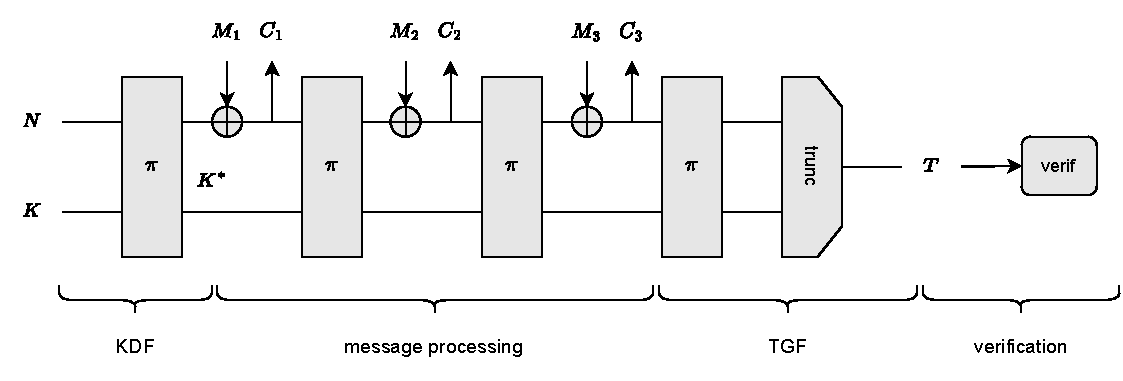
\includegraphics[width=12.0cm]{figures/mode_decomposition.pdf}
	\vspace*{0.3cm}
	\caption{Leakage-resistant modes of operation decomposition.}\label{fig:decomposition}\vspace*{-0.0cm}
\end{figure}

\medskip

The goal of this decomposition is to identify the parts of the modes
that must be implemented in a DPA-resistant manner and the parts of the modes that 
can be implemented with weaker guarantees. When analyzing confidentiality,
these weaker guarantees correspond to SPA security.
When analyzing integrity,
it is even possible to implement those parts without
any guarantee (which is referred to as the unbounded leakage model in
formal analyzes). We next classify the designs based on the amount of 
mode-level protections they embed.
At high-level (details are given in~\cite{DBLP:conf/crypto/BelliziaBCGGMPP20}),
Grade-0 designs do not provide mode-level leakage-resistance; Mode-1 designs
can be leveled to preserve confidentiality and integrity as long as only encryption
leakages are given to the adversary (i.e., CCAmL1 and CIML1); Mode-2 designs
can be leveled even if integrity with decryption leakage is required (i.e., CIML2); Mode-3 designs
complete the picture by allowing leveled implementations that preserve both confidentiality
and integrity with decryption leakages (i.e., CCAmL2 and CIML2).  

\subsubsection{Grade-0 designs (no mode-level protections).}
A first way to design modes of operation for lightweight cryptography 
is to focus exclusively on performance and to ignore leakage. This
is the case of modes where the long-term secret key is
used by most of the underlying primitives. In the NIST lightweight
crypto competition, it is for example what happens for
Elephant, GIFT-COFB, Romulus-N, Romulus-M and TinyJambu.
A protected implementation of Romulus-N targeting integrity with encryption leakage
is illustrated in Figure~\ref{fig:romulus_n},
where the blue color is used to reflect that the corresponding computations
must be protected against DPA. This requirement essentially holds for any security target (i.e., for confidentiality
and integrity, with or without nonce-misuse and leakage available in encryption or decryption).
We insist that being
Grade-0 does not imply that these modes cannot be protected against
leakage. It rather implies that this protection will be expensive
because uniformly applied to all the components of the modes.
The following (higher-level) designs gradually increase the mode-level protections,
leading to different trade-offs between the efficiency of their
unprotected implementations (that mildly decreases) and the efficiency
of their protected implementations (that significantly increases for long messages).


\begin{figure}
    \centering
    
    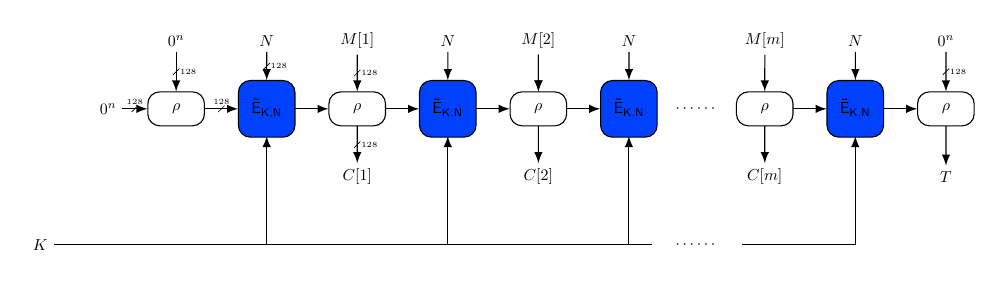
\begin{tikzpicture}[scale=0.575, every node/.style={transform shape}]
        \node (key) at (-3, -3) {$K$};
        \draw (-2.7, -3) -- (10.5, -3);
        \draw [-latex] (10,-3) -- (10, -0.6);
        \draw [-latex] (2,-3) -- (2, -0.6);
        \draw [-latex] (6,-3) -- (6, -0.6);
        \draw (12.5, -3) -- (15, -3);
        \draw [-latex] (15,-3) -- (15, -0.6);
        \node at (11.5,-3) {$\cdots\cdots$};

        \node (r0) at (0,0) [minimum size=1.25cm, minimum height = 0.75cm, rounded corners=1ex, draw] {$\rho$};
        \node (0) [above of=r0, node distance = 1.5cm] {$0^n$};
        \node (00) [left of=r0, node distance = 1.5cm] {$0^n$};
        \draw[next] (0) -- node {\bitwidth} node[bitwidthvert] {$128$} (r0);            
        \draw[next] (00) -- node {\bitwidth} node[bitwidth] {$128$} (r0);            

        \draw (2,0) \tencdpa{enc1};

        %\node (E1) [fill = blue!80, right of=r0, node distance=2cm, minimum size=1.25cm,rounded corners=1ex, draw] { $\tilde{E}_K^{26, 0}$};
        \node (n1) [above of=enc1, node distance = 1.5cm] {$N$};
        \draw[next] (n1) -- node {\bitwidth} node[bitwidthvert] {$128$} (enc1);            
        
        \draw[next] (r0) -- node {\bitwidth} node[bitwidth] {$128$} (enc1);            

        \node (r1) [right of=enc1, node distance=2cm, minimum size=1.25cm, minimum height = 0.75cm, rounded corners=1ex, draw] {$\rho$};
        \node (M1) [above of=r1, node distance = 1.5cm] {$M[1]$};
        \node (C1) [below of=r1, node distance = 1.5cm] {$C[1]$};

        \draw[-latex] (enc1) -- (r1);
        \draw[next] (M1) -- node {\bitwidth} node[bitwidthvert] {$128$} (r1);            
        \draw[next] (r1) -- node {\bitwidth} node[bitwidthvert] {$128$} (C1);            

        \draw (6,0) \tencdpa{enc2};
        \node (n2) [above of=enc2, node distance = 1.5cm] {$N$};
        \draw[-latex] (n2) -- (enc2);


        \draw[-latex] (r1) -- (enc2);
        \node (r2) [right of=enc2, node distance=2cm, minimum size=1.25cm, minimum height = 0.75cm, rounded corners=1ex, draw] {$\rho$};
        \node (M2) [above of=r2, node distance = 1.5cm] {$M[2]$};
        \node (C2) [below of=r2, node distance = 1.5cm] {$C[2]$};
        \draw[-latex] (enc2) -- (r2);
        \draw[-latex] (r2) -- (C2);
        \draw[-latex] (M2) -- (r2);

        \draw (10,0) \tencdpa{enc3};
        \draw[-latex] (r2) -- (enc3);
        \node (n3) [above of=enc3, node distance = 1.5cm] {$N$};
        \draw[-latex] (n3) -- (enc3);

        \begin{scope}
            \node at (11.5,0) {$\cdots\cdots$};
        \end{scope}
                    \draw[-latex] (M2) -- (r2);

        \node (r3) at (13,0) [minimum size=1.25cm, minimum height = 0.75cm, rounded corners=1ex, draw] {$\rho$};
        \node (Mm) [above of=r3, node distance = 1.5cm] {$M[m]$};
        \node (Cm) [below of=r3, node distance = 1.5cm] {$C[m]$};
        \draw[-latex] (r3) -- (Cm);
        \draw[-latex] (Mm) -- (r3);

        \draw (15,0) \tencdpa{E4};
        \node (n4) [above of=E4, node distance = 1.5cm] {$N$};
        \draw[-latex] (n4) -- (E4);
        \node (r4) [right of=E4, node distance=2cm, minimum size=1.25cm, minimum height = 0.75cm, rounded corners=1ex, draw] {$\rho$};
        \draw[-latex] (r3) -- (E4);
        \draw[-latex] (E4) -- (r4);

        \node (000) [above of=r4, node distance = 1.5cm] {$0^n$};
        \draw[next] (000) -- node {\bitwidth} node[bitwidthvert] {$128$} (r4);            
        \node (T) [below of=r4, node distance = 1.5cm] {$T$};
        \draw[-latex] (r4) -- (T);


    % PARENTHESING
                

    %\node (r) at (2,5cm, 0) [minimum size=1.5cm, minimum height=0.75cm, rounded corners=1ex, draw] {{$\rho$}};
    %\node (0) [above of=r, node distance=2.5cm] {$0^n$};
    %\node (00) [left of=r, node distance = 2.5cm] {$0^n$};
    %\draw[-latex] (0) -- (r);
    %\draw[-latex] (00) -- (r);


    %\node (enc_init) [right of=r, node distance = 2.5cm, minimum size = 2cm, rounded corners=1ex,fill=blue!20,draw] {{\sc $\tilde{E}_K$}};
    %\draw[-latex] (r) -- (enc_init);

\end{tikzpicture}


	\caption{Uniformly protected implementation of Romulus-N (integrity with encryption leakage).
	Blue blocks have to be secure against DPA.}
        \label{fig:romulus_n}\vspace*{-0.5cm}
\end{figure}

\subsubsection{Grade-1 designs (internal re-keying).} A first step towards
building modes of operation that cope better with leakage is to embed an internal
re-keying mechanism. In this case, the mode first generates a fresh
key $K^*$ from the long-term key and the nonce, which is then updated 
after the processing of each message block. As a result, and 
as long as the adversary can only observe encryption leakage 
without nonce misuse, only the KDF needs security against DPA (as there is
a DPA using the nonce) and all the other computations must only be protected 
against SPA. Such a leveled implementation is illustrated in Figure~\ref{fig:photon}
for PHOTON-Beetle. Unfortunately, this guarantee vanishes
as soon as nonce misuse or decryption leakage are granted to the adversary.
In this case the adversary can target the processing of one message block
with many different messages (while keeping the nonce and all the the other message blocks constant)
and perform a DPA to recover the corresponding intermediate state. In the
case of a P-sponge construction~\cite{Sponge07}, it is then possible to invert the permutation
and get back to the long-term key. 
In the NIST lightweight
crypto competition, it is the case of 
PHOTON-Beetle, Sparkle and Xoodyak.

\begin{figure}
    \centering
    \newif\ifsans
\newif\iftext
\newif\ifdetails

%%% CONFIGURATION %%%%%%%%%%%%%%%%%%%%%%%%%%%%%%%%%%%%%%%%%%%%%%%%%%%%%%%%%%%%%%%%
% preferably use build.py

%\sanstrue  % for sans-serif fonts (slides, web)
\sansfalse  % for serif fonts (article)

\textfalse  % include phase description
%\textfalse  % no phase description

\detailstrue % simplify (eg, 'const' instead of 'kab0'
%%%%%%%%%%%%%%%%%%%%%%%%%%%%%%%%%%%%%%%%%%%%%%%%%%%%%%%%%%%%%%%%%%%%%%%%%%%%%%%%%%

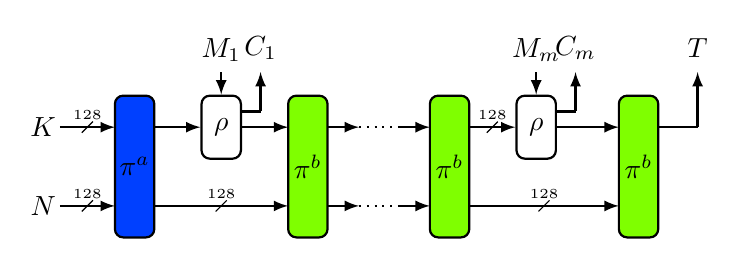
\begin{tikzpicture}[thick]


  % --- init up to p^a ---
  \begin{scope}[xshift=0cm]
      \draw (0,\rate) node[left, sparsam] {$K$};
      \draw (0,-\rate) node[left, sparsam] {$N$};
      \draw[next] (0,\rate) -- node {\bitwidth} node[bitwidth] {$128$} (.7,\rate);
      \draw[next] (0,-\rate) -- node {\bitwidth} node[bitwidth] {$128$} (.7,-\rate);


    \draw (.95,0) \permdpa{a};
  \end{scope}

  % --- init after p^a and auth A1 ---
  \begin{scope}[xshift=1.2cm]
    %\draw[next] (0,-\rate) -- (1.15,-\rate);
    \draw[next] (0, -\rate) -- node {\bitwidth} node [bitwidth] {$128$} + (1.7, 0);

    %\draw[dashdotted] (.8,1.5) -- (.8,-1.5);

    \draw (0.85,\rate) \ro{M1};
    \draw[-latex] (0,\rate) -- (M1);
    \draw[next] (M1) +(0,\msg) node[above] {$M_1$} -- (M1);
    \draw[next] (M1) -- (1.7,\rate);
    \draw(M1) +(0.25, 0.2) -- (1.35, 0.7);

    \draw[next] (1.35, 0.7) node at (1.35, 1.5) {$C_1$} -- (1.35, 1.2);
    \draw (1.95,0) \permspa{b};
  \end{scope}

  % --- auth As ---
  \begin{scope}[xshift=3.4cm]
    \draw[dotted] (\minnext,\rate) -- (0.9,\rate)
                  (\minnext,-\rate) -- (0.9,-\rate);

    \draw[next] (0,\rate) -- (\minnext, \rate);
    \draw[next] (0,-\rate) -- (\minnext, -\rate);
    
    \draw[next] (0.9,\rate) -- (1.3, \rate);
    \draw[next] (0.9,-\rate) -- (1.3, -\rate);

    \draw (1.55,0) \permspa{b};
  \end{scope}

  % --- enc P1 ---
  \begin{scope}[xshift=5.2cm]
    %\draw[next] (0,-\rate) -- (1.15,-\rate);
    \draw[next] (0, -\rate) -- node {\bitwidth} node [bitwidth] {$128$} + (1.9, 0);

    %\draw[dashdotted] (.8,1.5) -- (.8,-1.5);

    \draw (0.85,\rate) \ro{Mm};
    \draw[next] (0,\rate) -- node {\bitwidth} node[bitwidth] {$128$} (Mm);
    \draw[next] (Mm) +(0,\msg) node[above] {$M_m$} -- (Mm);
    \draw[next] (Mm) -- (1.9,\rate);
    \draw (Mm) +(0.25, 0.2) -- (1.35, 0.7);

    \draw[next] (1.35, 0.7) node at (1.35, 1.5) {$C_m$} -- (1.35, 1.2);
    \draw (2.15,0) \permspa{b};
  \end{scope}

  % --- enc Pt-1 ---
  \begin{scope}[xshift=7.6cm]
    \draw (0, \rate) -- (0.5, \rate);
    \draw[next] (0.5, \rate) node at (0.5, 1.5) {$T$} -- (0.5, 1.2);

  \end{scope}
    
\end{tikzpicture}

	\caption{Leveled implementation of PHOTON-Beetle (integrity with encryption leakage).
	Blue (resp., green) blocks have to be secure against DPA (resp., SPA).}
        \label{fig:photon}\vspace*{-0.5cm}
\end{figure}

\subsubsection{Grade-2 (Grade-1 + strengthened KDF/TGF).}
The second step towards
building modes of operation that cope better with leakage is to strengthen the
KDF/TGF so that the recovery of an internal state of the mode cannot
lead to long-term secrets. This is easily (and efficiently) done
by making the KDF and the TGF non-invertible. In the case of 
sponges, it can be achieved by XORing the long-term key before and
after the permutation used to generate the fresh key $K^*$ and the
tag $T$. For TBCs, it is a direct consequence of their PRP 
security. In the NIST lightweight
crypto competition, it is for example the case of 
Ascon. For illustration, its leveled implementation 
is illustrated in
Figure~\ref{fig:Ascon}.

\begin{figure}[h]
    \begin{subfigure}{\textwidth} \centering
	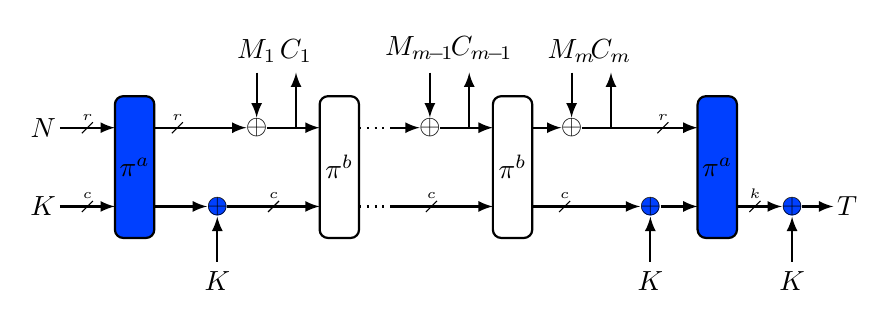
\begin{tikzpicture}[thick]
  % --- init up to p^a ---
  \begin{scope}[xshift=0cm]
      \draw (0,\rate) node[left, sparsam] {$N$};
      \draw (0,-\rate) node[left, sparsam] {$K$};

      \draw[next] (0,\rate) -- node {\bitwidth} node[bitwidth] {$r$} (.7,\rate);
      \draw[next] (0,-\rate) -- node {\bitwidth} node[bitwidth] {$c$} (.7,-\rate);



    \draw (.95,0) \permdpa{a};
  \end{scope}

  % --- enc P1 ---
  \begin{scope}[xshift=1.2cm]
    \draw (.8,-\rate) \xordpa{AuthPad};
    \draw[next] (0,-\rate) -- (AuthPad);
    \draw[next] (AuthPad) +(0,-\msg) node[below] {$K$} -- (AuthPad);
    \draw[next] (AuthPad) -- node {\bitwidth} node [bitwidth] {$c$} +(1.3, 0);

    %\draw[dashdotted] (.8,1.5) -- (.8,-1.5);

    \draw (1.3,\rate) \xor{P1};
    \draw[next] (0,\rate) -- node[near start] {\bitwidth} node[near start, bitwidth] {$r$} (P1);
    \draw[next] (P1) +(0,\msg) node[above] {$M_1$} -- (P1);
    \draw[next] (P1) -- +(2*\minnext,0);
    \draw[next] (P1) ++(.5,0) -- +(0,\msg) node[above] {$C_1$};

    \draw (2.35,0) \perm{b};
  \end{scope}

  % --- enc Pt-1 ---
  \begin{scope}[xshift=3.8cm]
    \draw[dotted] (0,\rate) -- (\minnext,\rate)
                  (0,-\rate) -- (\minnext,-\rate);

    \draw[next] (\minnext,-\rate) -- node[pos=.4] {\bitwidth} node [pos=.4,bitwidth] {$c$} +(1.3,0);

    \draw (.9,\rate) \xor{Pt1};
    \draw[next] (\minnext,\rate) -- (Pt1);
    \draw[next] (Pt1) +(0,\msg) node[above] {$M_{m\!-\!1}$ \hspace*{.15cm}} -- (Pt1);
    \draw[next] (Pt1) -- +(.8,0);
    \draw[next] (Pt1) ++(.5,0) -- +(0,\msg) node[above] {\hspace*{.2cm} $C_{m\!-\!1}$};

    \draw (1.95,0) \perm{b};
  \end{scope}

  % --- enc Pt and finalize ---
  \begin{scope}[xshift=6.0cm]
    \draw (.5,\rate) \xor{Pt};
    \draw[next] (0,\rate) -- (Pt);
    \draw[next] (Pt) +(0,\msg) node[above] {$M_m$} -- (Pt);
    \draw[next] (Pt) ++(.5,0) -- +(0,\msg) node[above] {$C_m$};
    \draw[next] (Pt) -- node[pos=.7] {\bitwidth} node[pos=.7,bitwidth] {$r$} +(1.6,0);

    %\draw[dashdotted] (1.3,1.5) -- (1.3,-1.5);

    \draw (1.5,-\rate) \xordpa{Kf};
    \draw[next] (Kf) +(0,-\msg) node[below] {$K$} -- (Kf);
    \draw[next] (0,-\rate) -- node[pos=.3] {\bitwidth} node[pos=.3,bitwidth] {$c$} (Kf);
    \draw[next] (Kf) -- (2.1,-\rate);

    \draw (2.35,0) \permdpa{a};

    \draw (3.3,-\rate) \xordpa{Kt};
    \draw[next] (Kt) +(0,-\msg) node[below] {$K$} -- (Kt);
    \draw[next] (2.6,-\rate) -- node[pos=.4] {\bitwidth} node[pos=.4,bitwidth] {$k$} (Kt);
    \draw (4.0,-\rate) node[name=T,sparsam] {$T$};
    \draw[next] (Kt) -- (T);
  \end{scope}

\end{tikzpicture}\caption{Integrity requirements (with decryption leakage).}
	\end{subfigure}
	\begin{subfigure}{\textwidth} \centering
	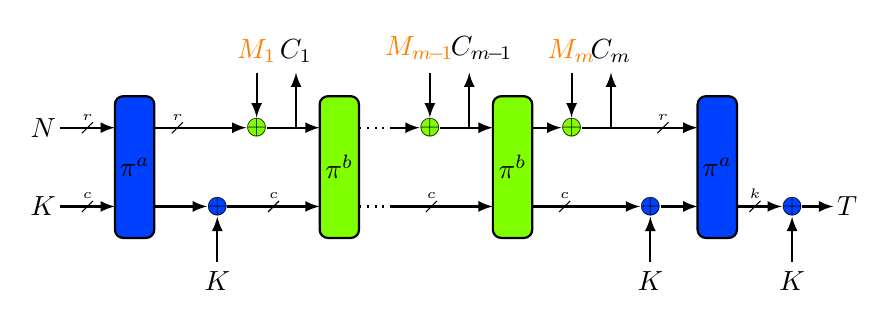
\begin{tikzpicture}[thick]
  % --- init up to p^a ---
  \begin{scope}[xshift=0cm]
      \draw (0,\rate) node[left, sparsam] {$N$};
      \draw (0,-\rate) node[left, sparsam] {$K$};

      \draw[next] (0,\rate) -- node {\bitwidth} node[bitwidth] {$r$} (.7,\rate);
      \draw[next] (0,-\rate) -- node {\bitwidth} node[bitwidth] {$c$} (.7,-\rate);



    \draw (.95,0) \permdpa{a};
  \end{scope}

  % --- enc P1 ---
  \begin{scope}[xshift=1.2cm]
    \draw (.8,-\rate) \xordpa{AuthPad};
    \draw[next] (0,-\rate) -- (AuthPad);
    \draw[next] (AuthPad) +(0,-\msg) node[below] {$K$} -- (AuthPad);
    \draw[next] (AuthPad) -- node {\bitwidth} node [bitwidth] {$c$} +(1.3, 0);

    %\draw[dashdotted] (.8,1.5) -- (.8,-1.5);

    \draw (1.3,\rate) \xorspa{P1};
    \draw[next] (0,\rate) -- node[near start] {\bitwidth} node[near start, bitwidth] {$r$} (P1);
    \draw[next] (P1) +(0,\msg) node[above, color = orange] {$M_1$} -- (P1);
    \draw[next] (P1) -- +(2*\minnext,0);
    \draw[next] (P1) ++(.5,0) -- +(0,\msg) node[above] {$C_1$};

    \draw (2.35,0) \permspa{b};
  \end{scope}

  % --- enc Pt-1 ---
  \begin{scope}[xshift=3.8cm]
    \draw[dotted] (0,\rate) -- (\minnext,\rate)
                  (0,-\rate) -- (\minnext,-\rate);

    \draw[next] (\minnext,-\rate) -- node[pos=.4] {\bitwidth} node [pos=.4,bitwidth] {$c$} +(1.3,0);

    \draw (.9,\rate) \xorspa{Pt1};
    \draw[next] (\minnext,\rate) -- (Pt1);
    \draw[next] (Pt1) +(0,\msg) node[above, color = orange] {$M_{m\!-\!1}$ \hspace*{.15cm}} -- (Pt1);
    \draw[next] (Pt1) -- +(.8,0);
    \draw[next] (Pt1) ++(.5,0) -- +(0,\msg) node[above] {\hspace*{.2cm} $C_{m\!-\!1}$};

    \draw (1.95,0) \permspa{b};
  \end{scope}

  % --- enc Pt and finalize ---
  \begin{scope}[xshift=6.0cm]
    \draw (.5,\rate) \xorspa{Pt};
    \draw[next] (0,\rate) -- (Pt);
    \draw[next] (Pt) +(0,\msg) node[above, color = orange] {$M_m$} -- (Pt);
    \draw[next] (Pt) ++(.5,0) -- +(0,\msg) node[above] {$C_m$};
    \draw[next] (Pt) -- node[pos=.7] {\bitwidth} node[pos=.7,bitwidth] {$r$} +(1.6,0);

    %\draw[dashdotted] (1.3,1.5) -- (1.3,-1.5);

    \draw (1.5,-\rate) \xordpa{Kf};
    \draw[next] (Kf) +(0,-\msg) node[below] {$K$} -- (Kf);
    \draw[next] (0,-\rate) -- node[pos=.3] {\bitwidth} node[pos=.3,bitwidth] {$c$} (Kf);
    \draw[next] (Kf) -- (2.1,-\rate);

    \draw (2.35,0) \permdpa{a};

    \draw (3.3,-\rate) \xordpa{Kt};
    \draw[next] (Kt) +(0,-\msg) node[below] {$K$} -- (Kt);
    \draw[next] (2.6,-\rate) -- node[pos=.4] {\bitwidth} node[pos=.4,bitwidth] {$k$} (Kt);
    \draw (4.0,-\rate) node[name=T,sparsam] {$T$};
    \draw[next] (Kt) -- (T);
  \end{scope}

\end{tikzpicture}\caption{Confidentiality requirements (without decryption leakage).}
	\end{subfigure}
        \caption{Leveled implementation of Ascon.
            The blue blocks have to be protected against DPA and the green blocks
            have to be protected against SPA, while the white ones do not require
            protection against side-channel leakage.
        }
        \label{fig:Ascon}
\end{figure}

\medskip

The top of the figure depicts the integrity requirements. In this case, only
the KDF and the TGF (in blue) must be protected against DPA  and the rest of the computations (in white)
can leak in full. This guarantee holds even when nonce misuse and
leakage in decryption are granted to the adversary. It intuitively derives
from the fact that the ephemeral secrets cannot be used to infer long-term ones,
and corresponds to the top of the hierarchy introduced in~\cite{DBLP:conf/latincrypt/GuoPPS19}.
The bottom of the figure 
depicts the confidentiality requirements. In this case, it is naturally 
not possible to tolerate unbounded leakage. Yet, as long as the adversary 
is not granted with decryption leakage, only SPA security (in green) is required 
for this part of the computation. (The orange color for the plaintexts
is used to reflect that even their very manipulation may leak sensitive information).
The main attack vector that remains against this construction happens
with decryption leakage. Since the message is decrypted before
verifying the tag, an adversary can then 
target the processing of one message block with many different
messages (keeping the nonce and all the the other message blocks constant) and perform
a DPA to recover the corresponding intermediate state.
This reveals the ephemeral keystream, hence the message, but does not
affect the confidentiality of messages encrypted with a different nonce.

\subsubsection{Grade-3 (Grade-2 + two passes).}
The natural way to get rid of the last attack vector against Ascon
is to consider 2-pass designs (such as encrypt-then-MAC constructions).
In this case, the tag can be computed
from the ciphertext blocks and tested before the decryption takes place. 
 In the NIST lightweight
crypto competition, it is for example the case of 
ISAP (which is permutation-based) and Romulus-T (which is TBC-based). 
Their main difference lies in the way they secure their KDF and TGF.
Like Ascon,
Romulus-T (which is based on the TEDT mode of operation~\cite{DBLP:journals/tches/BertiGPPS20})
relies on masking for this purpose. By contrast, ISAP relies on 
a leakage-resilient PRF. As illustrated in Figure~\ref{fig:ISAP}, the leakage-resilient PRF
can be viewed as a re-keying scheme where the nonce bits are absorbed one 
by one so that each of its intermediate keys is only used to process two 
permutation calls. As a result, this PRF essentially ``reduces'' DPA security to SPA 
security, at the cost of iterating the Ascon-p$^1$ permutation.\footnote{Increasing the rate 
to absorb more bits and get a more efficient design is possible but it then opens
a DPA attack vector (so we do not consider this option here).}

\begin{figure}
    \centering
    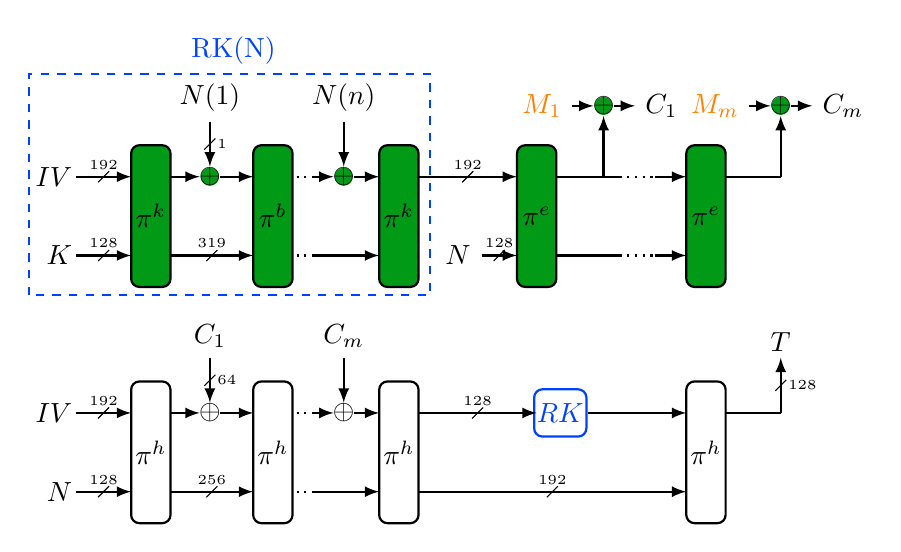
\begin{tikzpicture}[thick]

    % Draw RK box
    \draw [color = DPAblue] (2,2.1) node {RK(N)};
	\draw[thick,dashed, color = DPAblue] (-0.6, -1) rectangle ++(5.1,2.8);
  % --- init with IV, K ---
  \begin{scope}[xshift=0cm]
      \draw (0,\rate) node[left, sparsam] {$IV$};
      \draw (0,-\rate) node[left, sparsam] {$K$};

      \draw[next] (0,\rate) -- node {\bitwidth} node[bitwidth] {$192$} (.7,\rate);
      \draw[next] (0,-\rate) -- node {\bitwidth} node[bitwidth] {$128$} (.7,-\rate);

      \draw (.95,0) \permspav{k};
  \end{scope}

  % --- absorb N1 ---
  \begin{scope}[xshift=1cm]
    \draw[next] (0.2, -\rate) -- node {\bitwidth} node [bitwidth] {$319$} +(1.05,0);

    %\draw[dashdotted] (.8,1.5) -- (.8,-1.5);

    \draw (0.7,\rate) \xorspav{N1};
    \draw[-latex] (0.2,\rate) -- (N1);
    \draw[next] (N1) +(0,\msg) node[above] {$N(1)$} -- node {\bitwidth} node[bitwidthvert] {$1$} (N1);
    \draw[next] (N1) -- +(0.55,0);

    \draw (1.5,0) \permspav{b};
  \end{scope}

  % --- absorb Nn ---
  \begin{scope}[xshift=2.6cm]
    \draw[dotted] (0.2,\rate) -- (\minnext,\rate)
                  (0.2,-\rate) -- (\minnext,-\rate);

    \draw (.8,\rate) \xorspav{Nn};
    \draw[next] (\minnext,\rate) -- (Nn);
    \draw[next] (Nn) +(0,\msg) node[above] {$N(n)$} -- (Nn);
    \draw[next] (Nn) -- +(0.45,0);

    \draw[-latex] (\minnext,-\rate) -- (1.25,-\rate);

    \draw (1.5,0) \permspav{k};
  \end{scope}

  % --- Finish nonce absorption ---
  \begin{scope}[xshift=4.35cm]
  
    \draw (0.5, -\rate) node {$N$};
    \draw[next] (0.8,-\rate) -- node {\bitwidth} node[bitwidth] {$128$} (1.25, -\rate);

    %\draw[dashdotted] (.8,1.5) -- (.8,-1.5);

    \draw[next] (0,\rate) -- node{\bitwidth} node [bitwidth] {$192$} (1.25, \rate);

    \draw (1.5,0) \permspav{e};
  \end{scope}

  % --- enc M1 ---
  \begin{scope}[xshift=6.1cm]
    \draw (0,-\rate) -- (0.8, -\rate);

    \draw (0,\rate) -- (0.8, \rate);
    
    \draw (0.6, 1.4) \xorspav{Pt1};
    \draw[next] (0.6,\rate) -- (Pt1);
    \draw[next] (Pt1) +(-0.4, 0) node[left, color = orange] {$M_{1}$} -- (Pt1);
    \draw[next] (Pt1) -- +(0.4,0) node[right] {$C_{1}$};
    
    \draw[dotted] (0.8,\rate) -- (1.25,\rate)
                  (0.8,-\rate) -- (1.25,-\rate);
                  
    \draw[next] (1.25,-\rate) -- (1.65, -\rate);
    \draw[next] (1.25,\rate) -- (1.65, \rate);
    
    \draw (1.9,0) \permspav{e};
  \end{scope}

  % --- enc Mm ---
  \begin{scope}[xshift=8.25cm]

    \draw (0.7, 1.4) \xorspav{Pt1};
    \draw[next] (0.7,\rate) -- (Pt1);
    \draw (0, \rate) -- (0.7, \rate);
    \draw[next] (Pt1) +(-0.4, 0) node[left, color = orange] {$M_{m}$} -- (Pt1);
    \draw[next] (Pt1) -- +(0.4,0) node[right] {$C_{m}$};
  \end{scope}

    \begin{scope}[yshift=-3cm, xshift = 0cm]
      \draw (0,\rate) node[left, sparsam] {$IV$};
      \draw (0,-\rate) node[left, sparsam] {$N$};

      \draw[next] (0,\rate) -- node {\bitwidth} node[bitwidth] {$192$} (.7,\rate);
      \draw[next] (0,-\rate) -- node {\bitwidth} node[bitwidth] {$128$} (.7,-\rate);

      \draw (.95,0) \perm{h};

    \end{scope}
  \begin{scope}[yshift = -3cm, xshift=1cm]
    \draw[next] (0.2, -\rate) -- node {\bitwidth} node [bitwidth] {$256$} +(1.05,0);

    %\draw[dashdotted] (.8,1.5) -- (.8,-1.5);

    \draw (0.7,\rate) \xor{N1};
    \draw[-latex] (0.2,\rate) -- (N1);
    \draw[next] (N1) +(0,\msg) node[above] {$C_1$} -- node {\bitwidth} node[bitwidthvert] {$64$} (N1);
    \draw[next] (N1) -- +(0.55,0);

    \draw (1.5,0) \perm{h};
  \end{scope}
  
    \begin{scope}[yshift = -3cm, xshift=2.6cm]
    \draw[dotted] (0.2,\rate) -- (\minnext,\rate)
                  (0.2,-\rate) -- (\minnext,-\rate);

    \draw (.8,\rate) \xor{Nn};
    \draw[next] (\minnext,\rate) -- (Nn);
    \draw[next] (Nn) +(0,\msg) node[above] {$C_m$} -- (Nn);
    \draw[next] (Nn) -- +(0.45,0);

    \draw[-latex] (\minnext,-\rate) -- (1.25,-\rate);

    \draw (1.5,0) \perm{h};
  \end{scope}
  \begin{scope}[yshift = -3cm, xshift=4.35cm]

    %\draw[dashdotted] (.8,1.5) -- (.8,-1.5);
    
    \draw (1.8, \rate) node [rectangle, rounded corners=3pt, minimum width=.5cm, minimum height=.6cm, draw, sparsam, color = DPAblue] {$RK$};
    
    \draw[next] (0, \rate) -- node{\bitwidth} node [bitwidth] {$128$} (1.5, \rate);
    \draw[next] (0, -\rate) -- node{\bitwidth} node [bitwidth] {$192$} (3.4, -\rate);

  \end{scope}
  \begin{scope}[yshift=-3cm, xshift=6.1cm]
  
    \draw[next] (.4,\rate) -- (1.65, \rate);
    
    \draw (1.9,0) \perm{h};
  \end{scope}
  \begin{scope}[yshift=-3cm, xshift=8.25cm]
    \draw (0,\rate) -- (0.7, \rate);
    \draw[next] (0.7,\rate) -- node {\bitwidth} node [bitwidthvert] {$128$} (0.7, 1.2);
    \draw (0.7, 1.4)  node {$T$};
  \end{scope}

\end{tikzpicture}
	\caption{
            Leveled implementation of ISAP (confidentiality with decryption leakage).
            The green blocks have to be protected against SPA (with averaging), while the white
            ones do not require any protection against side-channel leakage.
        }\label{fig:ISAP}
\end{figure}

\begin{figure}
    \centering
    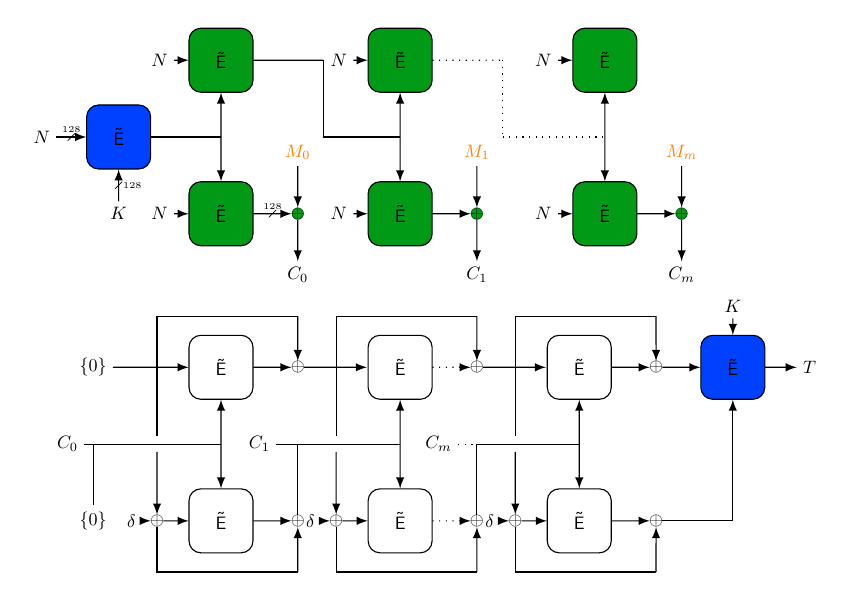
\begin{tikzpicture}[scale=0.65, every node/.style={transform shape}]

    \draw (1,0) \tbcdpa{enc1};
    \node (n) [left of=enc1, node distance = 1.5cm] {$N$};
    \node (k) [below of=enc1, node distance = 1.5cm] {$K$};
    \draw[next] (n) -- node {\bitwidth} node[bitwidth] {$128$} (enc1);            
    \draw[next] (k) -- node {\bitwidth} node[bitwidthvert] {$128$} (enc1); 
    \draw[] (enc1) -- (3,0);            
           
    \begin{scope}[xshift=0cm]
        \draw (3,1.5) \tbcspav{enc2};
        \node (n) [left of=enc2, node distance = 1.2cm] {$N$};
        \draw[next] (n) -- (enc2);            

        \draw (3,-1.5) \tbcspav{enc3};
        \node (n2) [left of=enc3, node distance = 1.2cm] {$N$};
        \draw[next] (n2) -- (enc3);            

        \draw (4.5, -1.5) \xorspav{m0};
        \node (m) [above of=m0, node distance = 1.2cm, color = orange] {$M_0$};
        \node (c) [below of=m0, node distance = 1.2cm] {$C_0$};
        \draw[next] (enc3) -- node {\bitwidth} node[bitwidth] {$128$} (m0);            
        \draw[next] (m) -- (m0);            
        \draw[next] (m0) -- (c);            
        \draw[next] (3, 0) -- (enc2);            
        \draw[next] (3, 0) -- (enc3); 
        \draw[] (enc2) -- (5,1.5);            
        \draw[] (5,1.5) -- (5, 0);            
        \draw[] (5,0) -- (6.5, 0);            
      
    \end{scope}
    \begin{scope}[xshift=3.5cm]
        \draw (3,1.5) \tbcspav{enc2};
        \node (n) [left of=enc2, node distance = 1.2cm] {$N$};
        \draw[next] (n) -- (enc2);            

        \draw (3,-1.5) \tbcspav{enc3};
        \node (n2) [left of=enc3, node distance = 1.2cm] {$N$};
        \draw[next] (n2) -- (enc3); 
        \draw (4.5, -1.5) \xorspav{m0};
        \node (m) [above of=m0, node distance = 1.2cm, color = orange] {$M_1$};
        \node (c) [below of=m0, node distance = 1.2cm] {$C_1$};
        \draw[next] (enc3) -- (m0);            
        \draw[next] (m) -- (m0);            
        \draw[next] (m0) -- (c);            
        \draw[next] (3, 0) -- (enc2);            
        \draw[next] (3, 0) -- (enc3); 
        \draw[dotted] (enc2) -- (5,1.5);            
        \draw[dotted] (5,1.5) -- (5, 0);            
        \draw[dotted] (5,0) -- (7, 0);            
      
    \end{scope}
    \begin{scope}[xshift=7.5cm]
        \draw (3,1.5) \tbcspav{enc2};
        \node (n) [left of=enc2, node distance = 1.2cm] {$N$};
        \draw[next] (n) -- (enc2);            

        \draw (3,-1.5) \tbcspav{enc3};
        \node (n2) [left of=enc3, node distance = 1.2cm] {$N$};
        \draw[next] (n2) -- (enc3); 
        \draw (4.5, -1.5) \xorspav{m0};
        \node (m) [above of=m0, node distance = 1.2cm, color = orange] {$M_m$};
        \node (c) [below of=m0, node distance = 1.2cm] {$C_m$};
        \draw[next] (enc3) -- (m0);            
        \draw[next] (m) -- (m0);            
        \draw[next] (m0) -- (c);            
        \draw[next] (3, 0) -- (enc2);            
        \draw[next] (3, 0) -- (enc3); 
    \end{scope}

    \begin{scope}[xshift=0cm, yshift = -6cm]
        \draw (3,1.5) \tbc{enc2};
        \node (L) [left of=enc2, node distance = 2.5cm] {$\{0\}$};
        \node (C) at (0,0) [] {$C_0$};
        \node (R) at (.5,-1.5) [] {$\{0\}$};
        \draw[] (R) |- (3, 0);            
        \draw[] (C) -- (3, 0);            

        \draw[next] (L) -- (enc2);            

        \draw (3,-1.5) \tbc{enc3};
        \draw (1.75, -1.5) \xor{deltax};
        \node (delta) [left of=deltax, node distance = .5cm] {$\delta$};

        \draw[next] (deltax) -- (enc3);            
        \draw[next] (delta) -- (deltax);   
        \draw[] (1.75,1.5) -- (1.75,.15);                     
        \draw[next] (1.75,-.15) -- (deltax);            

        \draw[] (1,0) -- (3,0);            
        \draw[next] (3,0) -- (enc3);            
        \draw[next] (3,0) -- (enc2);            

        \draw (4.5, 1.5) \xor{deltat};
        \draw[next] (enc2) -- (deltat);            
        \draw[] (1.75,1.5) |- (4.5, 2.5);            
        \draw[next] (4.5,2.5) -- (deltat);            
        \draw[next] (deltat) -- (5.85,1.5);            

        \draw (4.5, -1.5) \xor{deltat2};
        \draw[next] (enc3) -- (deltat2);            
        \draw[] (deltax) |- (4.5, -2.5);            
        \draw[next] (4.5,-2.5) -- (deltat2);            
        \draw[] (deltat2) |- (5,0);            



    \end{scope}

    \begin{scope}[xshift=3.5cm, yshift = -6cm]
        \draw (3,1.5) \tbc{enc2};
        \node (C) at (0.25,0) [] {$C_1$};
        \draw[] (deltat2) |- (3, 0);            
        \draw[] (C) -- (3, 0);            


        \draw (3,-1.5) \tbc{enc3};
        \draw (1.75, -1.5) \xor{deltax};
        \node (delta) [left of=deltax, node distance = .5cm] {$\delta$};

        \draw[next] (deltax) -- (enc3);            
        \draw[next] (delta) -- (deltax);   
        \draw[] (1.75,1.5) -- (1.75,.15);                     
        \draw[next] (1.75,-.15) -- (deltax);            

        \draw[] (1,0) -- (3,0);            
        \draw[next] (3,0) -- (enc3);            
        \draw[next] (3,0) -- (enc2);            

        \draw (4.5, 1.5) \xor{deltat};
        \draw[next, dotted] (enc2) -- (deltat);            
        \draw[] (1.75,1.5) |- (4.5, 2.5);            
        \draw[next] (4.5,2.5) -- (deltat);            
        \draw[next] (deltat) -- (5.85,1.5);            

        \draw (4.5, -1.5) \xor{deltat2};
        \draw[next, dotted] (enc3) -- (deltat2);            
        \draw[] (deltax) |- (4.5, -2.5);            
        \draw[next] (4.5,-2.5) -- (deltat2);            
        \draw[] (deltat2) |- (5,0);            

    \end{scope}
    \begin{scope}[xshift=7cm, yshift = -6cm]
        \draw (3,1.5) \tbc{enc2};

        \draw (3,-1.5) \tbc{enc3};
        \draw (1.75, -1.5) \xor{deltax};
        \node (delta) [left of=deltax, node distance = .5cm] {$\delta$};
        \draw (6,1.5) \tbcdpa{enc4};


        \draw[next] (deltax) -- (enc3);            
        \draw[next] (delta) -- (deltax);   
        \draw[] (1.75,1.5) -- (1.75,.15);                     
        \draw[next] (1.75,-.15) -- (deltax);            

        \draw[] (1,0) -- (3,0);            
        \draw[next] (3,0) -- (enc3);            
        \draw[next] (3,0) -- (enc2);            

        \draw (4.5, 1.5) \xor{deltat};
        \draw[next] (enc2) -- (deltat);            
        \draw[] (1.75,1.5) |- (4.5, 2.5);            
        \draw[next] (4.5,2.5) -- (deltat);            
        \draw[next] (deltat) -- (enc4);            

        \draw (4.5, -1.5) \xor{deltat2};
        \draw[next] (enc3) -- (deltat2);            
        \draw[] (deltax) |- (4.5, -2.5);            
        \draw[next] (4.5,-2.5) -- (deltat2);            
        \draw[next] (deltat2) -| (enc4);         

        \node (tag) [right of=enc4, node distance = 1.5cm] {$T$};
        \draw[next] (enc4) -- (tag);            
        \node (key) [above of=enc4, node distance = 1.2cm] {$K$};
        \draw[next] (key) -- (enc4);            

        \node (C) at (0.25,0) [] {$C_m$};
        \draw[dotted] (C) -- (3, 0);            


    \end{scope}
\end{tikzpicture}
    \caption{Leveled implementation of Romulus-T (confidentiality with decryption leakage).
            The blue blocks have to be protected against DPA and the green blocks
            have to be protected against SPA (with averaging), while the white ones do not require any
            protection against side-channel leakage.
    }
    \label{fig:TEDT}
\end{figure}

Overall, ISAP's confidentiality with decryption leakage requires two calls to the
leakage-resilient PRF and a plaintext processing that is secure against SPA.
We provide a similar picture for the leveled implementation
of Romulus-T in Figure~\ref{fig:TEDT}, where the KDF and TGF
are directly instantiated with a masked TBC. 
Note that the SPA-secure blocks of these two figures are in dark green to reflect the possibility
that the adversary repeats the same measurements to average the noise.
And as in the case of Ascon,
integrity with decryption leakage only requires the two protected calls (to 
the leakage-resilient PRF or masked TBC) and can let all the other computations leak in full.



\section{Hardware implementations}\label{sec:implem}

Given the previous analysis, it appears that Ascon, ISAP and Romulus-T are
the most promising candidates of the NIST lightweight crypto competition
for leakage-resistant implementations. In this section, we therefore investigate
their hardware implementations. For this purpose, we focus on
the security guarantees that they enable without a uniformly protected implementation.
We first investigate their primitives, with a special focus on Romulus-T
and its underlying TBC Skinny-384+ (for which, as mentioned in introduction,
the literature is a bit scarcer). We then detail the implementation of the
modes and report their performances (with ASIC synthesis). We use these results to confirm the
relevance of leveled implementations and to discuss the respective interest
of the three implemented ciphers in the context of the NIST competition.

\subsection{Masked implementation of the primitives}\label{subsec:prim}

We use the HPC2 masking scheme, as it allows almost arbitrary composition while
ensuring security against both hardware glitches and
transitions~\cite{DBLP:journals/tc/CassiersGLS21,DBLP:journals/tches/CassiersS21}.
The main characteristics of this masking scheme are the following.
The linear operations are very efficient, since they are made of purely
combinational logic and have a linear overhead in the masking order.
On the other hand, the non-linear operation, which is the 2-input AND gate (see
\autoref{algo:hpc2_mul}), has quadratic
overhead and asymmetric latency: 2~cycles with respect to one input, and only
1~cycle with respect to the other input.

\begin{algorithm}[tb]
    \caption{HPC2 AND gadget with $\nShares$ shares (sync. registers
    are omitted).}
    \label{algo:hpc2_mul}
    \begin{algorithmic}[1]
        \Require Sharings $\sharing{x}$, $\sharing{y}$
        \Ensure Sharing $\sharing{z}$ such that $z = x \cdot y$.
        \algrule
        \For{$i = 0 \text{ to }d-1$}
            \For{$j = i+1 \text{ to }d-1$}
                \State $r_{ij} \randtake \ft; \ r_{ji} \gets r_{ij}$
            \EndFor
        \EndFor
        \For{$i = 0 \text{ to }d-1$}
            \State $\share{z}{i} \gets \share{x}{i}\share{y}{i}$
            \For{$j = 0 \text{ to }d-1, j\neq i$}
                \State $\share{z}{i} \gets
                \share{z}{i} \oplus
                    \func{\reg}{\left(\share{x}{i}\oplus 1\right) r_{ij}}
                    \oplus \func{\reg}{\share{x}{i}\func{\reg}{\share{y}{j}\oplus r_{ij}}}
                    $
            \EndFor
        \EndFor
    \end{algorithmic}
\end{algorithm}


\subsubsection{Skinny Sbox.}\label{subsub:skinny_sbox}
The Skinny Sbox (depicted in \autoref{fig:sboxclean}) is made of XOR gates (that are
linear, and therefore easy to implement) and of NOR gates that we implement
with a AND gate whose inputs are inverted.

We next propose two area-optimized architectures for this Sbox, that both
instantiate two masked AND and two masked XOR gates.
\begin{figure}
    \centering
    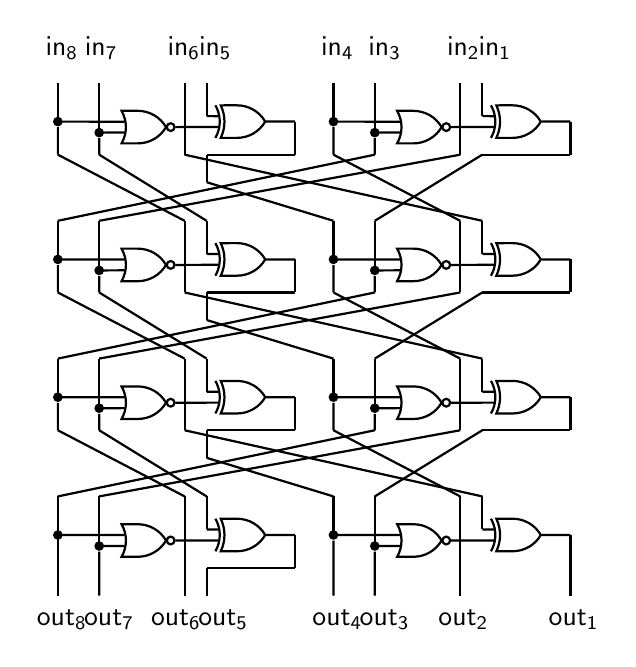
\begin{tikzpicture}[thick]
        \node [] (in_1) at (4.5, 1) {$\mathsf{in_{1}}$};
        \node [] (in_1) at (4.1, 1) {$\mathsf{in_{2}}$};
        \node [] (in_1) at (3.1, 1) {$\mathsf{in_{3}}$};
        \node [] (in_1) at (2.5, 1) {$\mathsf{in_{4}}$};
        \node [] (in_1) at (.95, 1) {$\mathsf{in_{5}}$};
        \node [] (in_1) at (0.55, 1) {$\mathsf{in_{6}}$};
        \node [] (in_1) at (-.5, 1) {$\mathsf{in_{7}}$};
        \node [] (in_1) at (-1, 1) {$\mathsf{in_{8}}$};

        \node [] (in_1) at (5.5, -6.25) {$\mathsf{out_{1}}$};
        \node [] (in_1) at (4.1, -6.25) {$\mathsf{out_{2}}$};
        \node [] (in_1) at (3.1, -6.25) {$\mathsf{out_{3}}$};
        \node [] (in_1) at (2.5, -6.25) {$\mathsf{out_{4}}$};
        \node [] (in_1) at (1.05, -6.25) {$\mathsf{out_{5}}$};
        \node [] (in_1) at (.45, -6.25) {$\mathsf{out_{6}}$};
        \node [] (in_1) at (-.4, -6.25) {$\mathsf{out_{7}}$};
        \node [] (in_1) at (-1, -6.25) {$\mathsf{out_{8}}$};
        
        \begin{scope}[scale=.7, every node/.style={transform shape}]
                
                \begin{scope}[yshift = 0cm]
                        \begin{scope}
                                \node[nor gate US, draw] at (0,0) (nor1) {};
                                \node[xor gate US, draw] at ($(nor1) + (1.8, 0.1)$) (xor1) {};
                                
                                \draw (nor1.output) -- (xor1.input 2);
                                \draw (-1.5, .1) -- (nor1.input 1);
                                \draw (-.75, -.1) -- (nor1.input 2);
                                \draw (1.2, .2) -- (xor1.input 1);
                                \draw (xor1.output) -- (2.8, .1);

                                \node[contact] (c1) at (-1.5,.1){};
                                \node[contact] (c2) at (-.75,-.1){};

                                % Input lines
                                \draw (-1.5,.8) -- (-1.5, .1);
                                \draw (-.75,.8) -- (-.75, -.1);
                                \draw (1.2, .8) -- (1.2, .2);
                                \draw (.8, .8) -- (.8, -.5);
                                % 1st input
                                \draw (c1) -- (-1.5, -.5);
                                \draw (-1.5, -.5) -- (.8, -1.7);
                                % 2nd input 
                                \draw (c2) -- (-.75, -.5);
                                \draw (-.75, -.5) -- (1.2, -1.7);
                                % 3rd input
                                \draw (.8, -.5) -- (6.2, -1.7);
                                % output
                                \draw (2.8,.1) -- (2.8, -.5);
                                \draw (2.8, -.5) -- (1.2, -.5);
                                \draw (1.2, -.5) -- (1.2, -1);
                                \draw (1.2, -1) -- (3.5, -1.7);


                        \end{scope}
                        \begin{scope}[xshift = 5cm]
                                \node[nor gate US, draw] at (0,0) (nor1) {};
                                \node[xor gate US, draw] at ($(nor1) + (1.8, 0.1)$) (xor1) {};
                                
                                \draw (nor1.output) -- (xor1.input 2);
                                \draw (-1.5, .1) -- (nor1.input 1);
                                \draw (-.75, -.1) -- (nor1.input 2);
                                \draw (1.2, .2) -- (xor1.input 1);
                                \draw (xor1.output) -- (2.8, .1);

                                \node[contact] (c1) at (-1.5,.1){};
                                \node[contact] (c2) at (-.75,-.1){};

                                % Input lines
                                \draw (-1.5,.8) -- (-1.5, .1);
                                \draw (-.75,.8) -- (-.75, -.1);
                                \draw (1.2, .8) -- (1.2, .2);
                                \draw (.8, .8) -- (.8, -.5);
                                % 3rd input
                                \draw (.8, -.5) -- (-5.75, -1.7);
                                % 2nd input
                                \draw (c2) -- (-.75, -.5);
                                \draw (-.75, -.5) -- (-6.5, -1.7);
                                % 1st input
                                \draw (c1) -- (-1.5, -.5);
                                \draw (-1.5, -.5) -- (.8, -1.7);
                                % output
                                \draw (2.8,.1) -- (2.8, -.5);
                                \draw (2.8, -.5) -- (1.2, -.5);
                                \draw (1.2, -.5) -- (-.75, -1.7);
                                
                                
                        \end{scope}
                \end{scope}
                \begin{scope}[yshift = -2.5cm]
                        \begin{scope}
                                \node[nor gate US, draw] at (0,0) (nor1) {};
                                \node[xor gate US, draw] at ($(nor1) + (1.8, 0.1)$) (xor1) {};
                                
                                \draw (nor1.output) -- (xor1.input 2);
                                \draw (-1.5, .1) -- (nor1.input 1);
                                \draw (-.75, -.1) -- (nor1.input 2);
                                \draw (1.2, .2) -- (xor1.input 1);
                                \draw (xor1.output) -- (2.8, .1);

                                \node[contact] (c1) at (-1.5,.1){};
                                \node[contact] (c2) at (-.75,-.1){};

                                % Input lines
                                \draw (-1.5,.8) -- (-1.5, .1);
                                \draw (-.75,.8) -- (-.75, -.1);
                                \draw (1.2, .8) -- (1.2, .2);
                                \draw (.8, .8) -- (.8, -.5);
                                % 1st input
                                \draw (c1) -- (-1.5, -.5);
                                \draw (-1.5, -.5) -- (.8, -1.7);
                                % 2nd input 
                                \draw (c2) -- (-.75, -.5);
                                \draw (-.75, -.5) -- (1.2, -1.7);
                                % 3rd input
                                \draw (.8, -.5) -- (6.2, -1.7);
                                % output
                                \draw (2.8,.1) -- (2.8, -.5);
                                \draw (2.8, -.5) -- (1.2, -.5);
                                \draw (1.2, -.5) -- (1.2, -1);
                                \draw (1.2, -1) -- (3.5, -1.7);


                        \end{scope}
                        \begin{scope}[xshift = 5cm]
                                \node[nor gate US, draw] at (0,0) (nor1) {};
                                \node[xor gate US, draw] at ($(nor1) + (1.8, 0.1)$) (xor1) {};
                                
                                \draw (nor1.output) -- (xor1.input 2);
                                \draw (-1.5, .1) -- (nor1.input 1);
                                \draw (-.75, -.1) -- (nor1.input 2);
                                \draw (1.2, .2) -- (xor1.input 1);
                                \draw (xor1.output) -- (2.8, .1);

                                \node[contact] (c1) at (-1.5,.1){};
                                \node[contact] (c2) at (-.75,-.1){};

                                % Input lines
                                \draw (-1.5,.8) -- (-1.5, .1);
                                \draw (-.75,.8) -- (-.75, -.1);
                                \draw (1.2, .8) -- (1.2, .2);
                                \draw (.8, .8) -- (.8, -.5);
                                % 3rd input
                                \draw (.8, -.5) -- (-5.75, -1.7);
                                % 2nd input
                                \draw (c2) -- (-.75, -.5);
                                \draw (-.75, -.5) -- (-6.5, -1.7);
                                % 1st input
                                \draw (c1) -- (-1.5, -.5);
                                \draw (-1.5, -.5) -- (.8, -1.7);
                                % output
                                \draw (2.8,.1) -- (2.8, -.5);
                                \draw (2.8, -.5) -- (1.2, -.5);
                                \draw (1.2, -.5) -- (-.75, -1.7);
                                
                                
                        \end{scope}                
                \end{scope}                
                \begin{scope}[yshift = -5cm]
                        \begin{scope}
                                \node[nor gate US, draw] at (0,0) (nor1) {};
                                \node[xor gate US, draw] at ($(nor1) + (1.8, 0.1)$) (xor1) {};
                                
                                \draw (nor1.output) -- (xor1.input 2);
                                \draw (-1.5, .1) -- (nor1.input 1);
                                \draw (-.75, -.1) -- (nor1.input 2);
                                \draw (1.2, .2) -- (xor1.input 1);
                                \draw (xor1.output) -- (2.8, .1);

                                \node[contact] (c1) at (-1.5,.1){};
                                \node[contact] (c2) at (-.75,-.1){};

                                % Input lines
                                \draw (-1.5,.8) -- (-1.5, .1);
                                \draw (-.75,.8) -- (-.75, -.1);
                                \draw (1.2, .8) -- (1.2, .2);
                                \draw (.8, .8) -- (.8, -.5);
                                % 1st input
                                \draw (c1) -- (-1.5, -.5);
                                \draw (-1.5, -.5) -- (.8, -1.7);
                                % 2nd input 
                                \draw (c2) -- (-.75, -.5);
                                \draw (-.75, -.5) -- (1.2, -1.7);
                                % 3rd input
                                \draw (.8, -.5) -- (6.2, -1.7);
                                % output
                                \draw (2.8,.1) -- (2.8, -.5);
                                \draw (2.8, -.5) -- (1.2, -.5);
                                \draw (1.2, -.5) -- (1.2, -1);
                                \draw (1.2, -1) -- (3.5, -1.7);


                        \end{scope}
                        \begin{scope}[xshift = 5cm]
                                \node[nor gate US, draw] at (0,0) (nor1) {};
                                \node[xor gate US, draw] at ($(nor1) + (1.8, 0.1)$) (xor1) {};
                                
                                \draw (nor1.output) -- (xor1.input 2);
                                \draw (-1.5, .1) -- (nor1.input 1);
                                \draw (-.75, -.1) -- (nor1.input 2);
                                \draw (1.2, .2) -- (xor1.input 1);
                                \draw (xor1.output) -- (2.8, .1);

                                \node[contact] (c1) at (-1.5,.1){};
                                \node[contact] (c2) at (-.75,-.1){};

                                % Input lines
                                \draw (-1.5,.8) -- (-1.5, .1);
                                \draw (-.75,.8) -- (-.75, -.1);
                                \draw (1.2, .8) -- (1.2, .2);
                                \draw (.8, .8) -- (.8, -.5);
                                % 3rd input
                                \draw (.8, -.5) -- (-5.75, -1.7);
                                % 2nd input
                                \draw (c2) -- (-.75, -.5);
                                \draw (-.75, -.5) -- (-6.5, -1.7);
                                % 1st input
                                \draw (c1) -- (-1.5, -.5);
                                \draw (-1.5, -.5) -- (.8, -1.7);
                                % output
                                \draw (2.8,.1) -- (2.8, -.5);
                                \draw (2.8, -.5) -- (1.2, -.5);
                                \draw (1.2, -.5) -- (-.75, -1.7);
                                
                                
                        \end{scope}
                \end{scope}                
                \begin{scope}[yshift = -7.5cm]
                        \begin{scope}
                                \node[nor gate US, draw] at (0,0) (nor1) {};
                                \node[xor gate US, draw] at ($(nor1) + (1.8, 0.1)$) (xor1) {};
                                
                                \draw (nor1.output) -- (xor1.input 2);
                                \draw (-1.5, .1) -- (nor1.input 1);
                                \draw (-.75, -.1) -- (nor1.input 2);
                                \draw (1.2, .2) -- (xor1.input 1);
                                \draw (xor1.output) -- (2.8, .1);

                                \node[contact] (c1) at (-1.5,.1){};
                                \node[contact] (c2) at (-.75,-.1){};

                                % Input lines
                                \draw (-1.5,.8) -- (-1.5, .1);
                                \draw (-.75,.8) -- (-.75, -.1);
                                \draw (1.2, .8) -- (1.2, .2);
                                \draw (.8, .8) -- (.8, -1);
                                % output
                                \draw (2.8,.1) -- (2.8, -.5);
                                \draw (2.8, -.5) -- (1.2, -.5);
                                \draw (1.2, -.5) -- (1.2, -1);
                                % ouput first bit
                                \draw (-1.5, .1) -- (-1.5, -1);
                                % output second bit
                                \draw (c2) -- (-.75, -1);
                                
                        \end{scope}
                        \begin{scope}[xshift = 5cm]
                                \node[nor gate US, draw] at (0,0) (nor1) {};
                                \node[xor gate US, draw] at ($(nor1) + (1.8, 0.1)$) (xor1) {};
                                
                                \draw (nor1.output) -- (xor1.input 2);
                                \draw (-1.5, .1) -- (nor1.input 1);
                                \draw (-.75, -.1) -- (nor1.input 2);
                                \draw (1.2, .2) -- (xor1.input 1);
                                \draw (xor1.output) -- (2.8, .1);

                                \node[contact] (c1) at (-1.5,.1){};
                                \node[contact] (c2) at (-.75,-.1){};

                                % Input lines
                                \draw (-1.5,.8) -- (-1.5, .1);
                                \draw (-.75,.8) -- (-.75, -.1);
                                \draw (1.2, .8) -- (1.2, .2);
                                \draw (.8, .8) -- (.8, -1);
                                % 3rd input
                                % 2nd input
                                \draw (c2) -- (-.75, -1);
                                % 1st input
                                \draw (c1) -- (-1.5, -1);
                                % output
                                \draw (2.8,.1) -- (2.8, -1);
                                
                                
                        \end{scope}
                \end{scope}
        \end{scope}

        \end{tikzpicture}
    \caption{Skinny Sbox circuit representation with NOR and XOR gates.}
    \label{fig:sboxclean}
\end{figure}
First, the high-throughput one is based on the observation that the Sbox can be
decomposed into 4~applications of a simpler function (as visible in
\autoref{fig:sboxclean}), followed by a wire shuffling.
This function has a latency of at least two cycles with our masking
scheme, due to the AND gate.
We therefore build the high-throughput Sbox by looping 4~times on a two-stage
pipeline.
The core of this pipeline is a simple function block B shown in
\autoref{fig:block}, which is then used twice and connected to combinational
logic to form the Sbox (\autoref{fig:sboxser_circuit}).
The two-stage pipeline can be used to perform simultaneously two Sbox
operations.
We finally add input and output synchronization registers such that the logic
performs two Sbox evaluations in 9~clock cycles, without the need for any
external synchronization mechanism.
\begin{figure}
	\begin{subfigure}[b]{.48\textwidth}
		\centering
		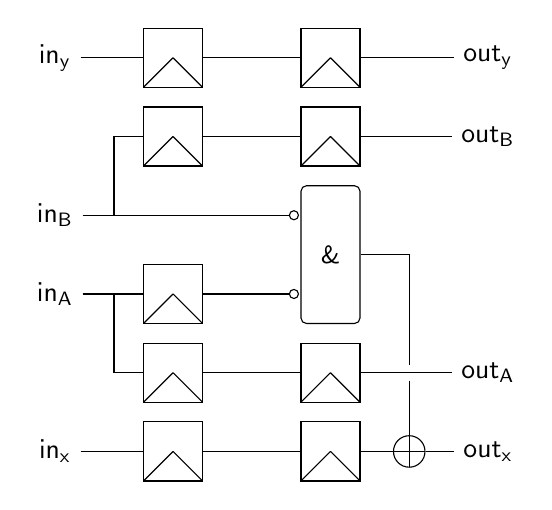
\begin{tikzpicture}[]
  %\draw [] (0, 0) \register{reg1};
  \draw [] (0, 1) \register{reg1};
  \draw [] (2, 1) \register{reg2};
  \draw [] (0, 3) \register{reg3};
  \draw [] (0, 6) \register{reg4};
  \draw [] (2, 6) \register{reg5};
  \draw [] (0, 5) \register{reg6};
  \draw [] (2, 5) \register{reg7};
  \draw [] (0, 2) \register{reg8};
  \draw [] (2, 2) \register{reg9};

  \draw [] (3, 1) \xord{xor1};

  \node[rectangle,
  minimum width = .75cm,
  minimum height = 1.75cm,
  draw,
  rounded corners = 2pt
  ] (B2) at (2,3.5) {\small \textsf{\&}};

  \node [] (ina) at (-1.5, 3) {$\mathsf{in}_\mathsf{A}$};
  \node [] (inb) at (-1.5, 4) {$\mathsf{in}_\mathsf{B}$};
  \node [] (inx) at (-1.5, 1) {$\mathsf{in_x}$};
  \node [] (iny) at (-1.5, 6) {$\mathsf{in_y}$};

  \node [] (outx) at (4, 1) {$\mathsf{out_x}$};
  \node [] (outa) at (4, 2) {$\mathsf{out_A}$};
  \node [] (outb) at (4, 5) {$\mathsf{out_B}$};
  \node [] (outz) at (4, 6) {$\mathsf{out_y}$};

  \draw[] (iny) -- (reg4);
  \draw[] (reg4) -- (reg5);
  \draw[] (reg5) -- (outz);

  \draw[] (ina) -- (reg3);
  \draw[{-Circle[open]}] (inb) -- (1.6,4);
  \draw[{-Circle[open]}] (reg3) -- (1.6,3);
  \draw[] (inx) -- (reg1);
  \draw[] (reg1) -- (reg2);
  \draw[] (reg2) -- (xor1);
  \draw[] (B2) -| (3,2.1);
  \draw[] (3, 1.9) -- (xor1);
  \draw[] (xor1) -- (outx);

    \draw[] (-.75,4) -- (-.75, 5);
    \draw[] (-.75,5) -- (reg6);
    \draw[] (reg6) -- (reg7);
    \draw[] (reg7) -- (outb);

    \draw[] (-.75,3) -- (-.75, 2);
    \draw[] (-.75,2) -- (reg8);
    \draw[] (reg8) -- (reg9);
    \draw[] (reg9) -- (outa);

\end{tikzpicture}
		\caption{%
                    Inner logic block ``B'' for Sbox implementation, with one
                    AND and one XOR.
                }
                \label{fig:block}
	\end{subfigure}
        \hfill
	\begin{subfigure}[b]{.48\textwidth}
		\centering
		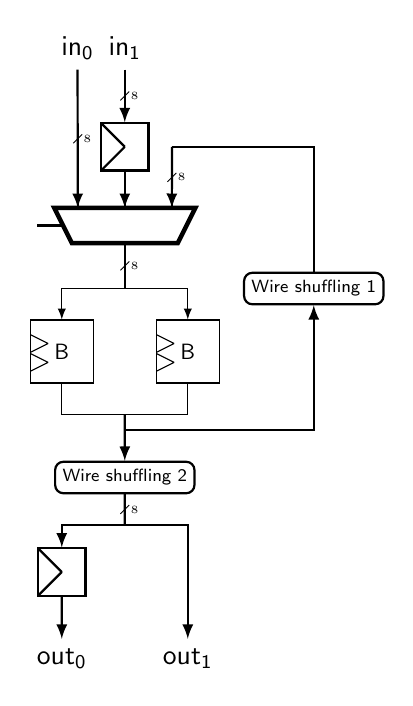
\begin{tikzpicture}[]
    \node [] (in1) at (-.6, 2.25) {$\mathsf{in_0}$};
    \node [] (in0) at (0, 2.25) {$\mathsf{in_1}$};
    \node [] (o1) at (-.8, -5.5) {$\mathsf{out_0}$};
    \node [] (o0) at (.8, -5.5) {$\mathsf{out_1}$};
\begin{scope}[scale=.8, every node/.style={transform shape}]
    
    \node[rectangle,
    latency,
    minimum width = 1cm,
    minimum height = 1cm,
    draw] (B1) at (-1,-2) {\textsf{B}};

    \draw [thick] (0, 1.25) \registerrot{reg1};
    \draw [thick] (-1, -5.5) \registerrot{reg2};

    \node[rectangle,
    latency,
    minimum width = 1cm,
    minimum height = 1cm,
    draw,
    ] (B2) at (1,-2) {\textsf{B}};

    \node [mux 3by2, rotate = 270, thick](M1) at (0, 0){};

    \node[rectangle,
    minimum width = 1cm,
    rounded corners = 3pt,
    thick,
    minimum height = .5cm,
    draw] (ws1) at (0, -4) {\footnotesize \textsf{Wire shuffling 2}};

    \node[rectangle,
    minimum width = 1cm,
    rounded corners = 3pt,
    thick,
    minimum height = .5cm,
    draw] (ws2) at (3,-1) {\footnotesize \textsf{Wire shuffling 1}};

    \draw [thick, -latex] (0, -3.25) -| (ws2);
    \draw [thick] (M1.brpin 1) -- node {\bitwidth} node [bitwidthvert] {8} (0, -1);
    \draw [-latex, thick] (reg1) -- (M1.blpin 2);
    \draw [-latex, thick] (in1) -- node {\bitwidth} node [bitwidthvert] {8} (M1.blpin 3);

    \draw [-latex, thick] (in0) -- node {\bitwidth} node [bitwidthvert] {8} (reg1);
    \draw [-latex] (0, -1) -| (B1);
    \draw [-latex] (0, -1) -| (B2);
    \draw [] (B1) |- (0, -3);
    \draw [] (B2) |- (0, -3);
    \draw [thick, -latex] (0, -3) -- (ws1);
    \draw [thick] (ws2) |- (.75,1.25);
    \draw [thick, -latex] (.75, 1.25) -- node {\bitwidth} node [bitwidthvert] {8} (M1.blpin 1);

    \draw [thick] (ws1) -- node {\bitwidth} node [bitwidthvert] {8} (0, -4.75);
    \draw [-latex, thick] (0,-4.75) -| (reg2);

    \draw [-latex, thick] (0, -4.75) -| (o0);
    \draw [-latex, thick] (reg2) -- (o1);
\end{scope}

\end{tikzpicture}
		\caption{%
                    High-throughput Sbox architecture with input and output
                    sync. registers.
                }
                \label{fig:sboxser_circuit}
	\end{subfigure}
	\caption{%
            High-throughput masked Skinny Sbox.
        }
        \label{fig:sboxintro}
\end{figure}
Second, we design a low-latency architecture with an ALU-style design: the Sbox
inputs are stored in a register, as well as the outputs, and the data fed to
the two AND-XOR blocks are selected from these states (and from the input
wires) when needed (see \autoref{fig:sboxopt_circuit}).
This flexible architecture allows to benefit from the asymmetric latency of the
HPC2 AND gadgets, leading to a latency of 6~cycles for one Sbox evaluation (see
\autoref{fig:sbox_opt}).

\begin{figure}
    \begin{subfigure}[b]{.48\textwidth}
        \centering
        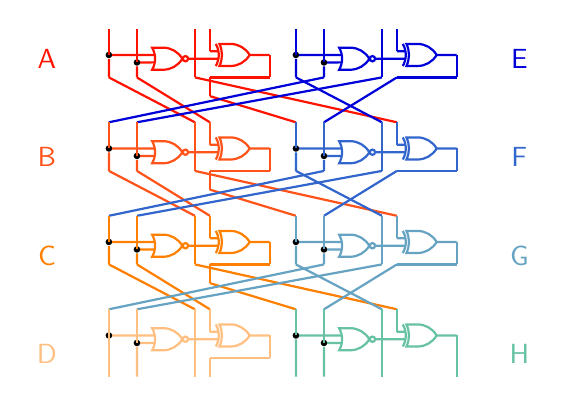
\begin{tikzpicture}[thick]
\begin{scope}
        
        \node [color = red!85!orange] (block1) at (-1.5, 0) {$\mathsf{A}$};
        \node [color = red!50!orange!90!white] (block2) at (-1.5, -1.25) {$\mathsf{B}$};
        \node [color = orange] (block3) at (-1.5, -2.5) {$\mathsf{C}$};
        \node [color = orange!50!white] (block1) at (-1.5, -3.75) {$\mathsf{D}$};
        \node [color = blue!85!black] (block1) at (4.5, 0) {$\mathsf{E}$};
        \node [color = blue!75!green!80!white] (block2) at (4.5, -1.25) {$\mathsf{F}$};
        \node [color = green!40!blue!60!white] (block3) at (4.5, -2.5) {$\mathsf{G}$};
        \node [color = green!60!blue!60!white] (block1) at (4.5, -3.75) {$\mathsf{H}$};

\end{scope}

        \begin{scope}[scale=0.475, every node/.style={transform shape}]
                
                \begin{scope}[yshift = 0cm]
                        \begin{scope}[color = red!85!orange]
                                \node[nor gate US, draw] at (0,0) (nor1) {};
                                \node[xor gate US, draw] at ($(nor1) + (1.8, 0.1)$) (xor1) {};
                                
                                \draw (nor1.output) -- (xor1.input 2);
                                \draw (-1.5, .1) -- (nor1.input 1);
                                \draw (-.75, -.1) -- (nor1.input 2);
                                \draw (1.2, .2) -- (xor1.input 1);
                                \draw (xor1.output) -- (2.8, .1);

                                \node[contact] (c1) at (-1.5,.1){};
                                \node[contact] (c2) at (-.75,-.1){};

                                % Input lines
                                \draw (-1.5,.8) -- (-1.5, .1);
                                \draw (-.75,.8) -- (-.75, -.1);
                                \draw (1.2, .8) -- (1.2, .2);
                                \draw (.8, .8) -- (.8, -.5);
                                % 1st input
                                \draw (c1) -- (-1.5, -.5);
                                \draw (-1.5, -.5) -- (.8, -1.7);
                                % 2nd input 
                                \draw (c2) -- (-.75, -.5);
                                \draw (-.75, -.5) -- (1.2, -1.7);
                                % 3rd input
                                \draw (.8, -.5) -- (6.2, -1.7);
                                % output
                                \draw (2.8,.1) -- (2.8, -.5);
                                \draw (2.8, -.5) -- (1.2, -.5);
                                \draw (1.2, -.5) -- (1.2, -1);
                                \draw (1.2, -1) -- (3.5, -1.7);


                        \end{scope}
                        \begin{scope}[xshift = 5cm, color = blue!85!black]
                                \node[nor gate US, draw] at (0,0) (nor1) {};
                                \node[xor gate US, draw] at ($(nor1) + (1.8, 0.1)$) (xor1) {};
                                
                                \draw (nor1.output) -- (xor1.input 2);
                                \draw (-1.5, .1) -- (nor1.input 1);
                                \draw (-.75, -.1) -- (nor1.input 2);
                                \draw (1.2, .2) -- (xor1.input 1);
                                \draw (xor1.output) -- (2.8, .1);

                                \node[contact] (c1) at (-1.5,.1){};
                                \node[contact] (c2) at (-.75,-.1){};

                                % Input lines
                                \draw (-1.5,.8) -- (-1.5, .1);
                                \draw (-.75,.8) -- (-.75, -.1);
                                \draw (1.2, .8) -- (1.2, .2);
                                \draw (.8, .8) -- (.8, -.5);
                                % 3rd input
                                \draw (.8, -.5) -- (-5.75, -1.7);
                                % 2nd input
                                \draw (c2) -- (-.75, -.5);
                                \draw (-.75, -.5) -- (-6.5, -1.7);
                                % 1st input
                                \draw (c1) -- (-1.5, -.5);
                                \draw (-1.5, -.5) -- (.8, -1.7);
                                % output
                                \draw (2.8,.1) -- (2.8, -.5);
                                \draw (2.8, -.5) -- (1.2, -.5);
                                \draw (1.2, -.5) -- (-.75, -1.7);
                                
                                
                        \end{scope}
                \end{scope}
                \begin{scope}[yshift = -2.5cm, color = red!50!orange!90!white]
                        \begin{scope}
                                \node[nor gate US, draw] at (0,0) (nor1) {};
                                \node[xor gate US, draw] at ($(nor1) + (1.8, 0.1)$) (xor1) {};
                                
                                \draw (nor1.output) -- (xor1.input 2);
                                \draw (-1.5, .1) -- (nor1.input 1);
                                \draw (-.75, -.1) -- (nor1.input 2);
                                \draw (1.2, .2) -- (xor1.input 1);
                                \draw (xor1.output) -- (2.8, .1);

                                \node[contact] (c1) at (-1.5,.1){};
                                \node[contact] (c2) at (-.75,-.1){};

                                % Input lines
                                \draw (-1.5,.8) -- (-1.5, .1);
                                \draw (-.75,.8) -- (-.75, -.1);
                                \draw (1.2, .8) -- (1.2, .2);
                                \draw (.8, .8) -- (.8, -.5);
                                % 1st input
                                \draw (c1) -- (-1.5, -.5);
                                \draw (-1.5, -.5) -- (.8, -1.7);
                                % 2nd input 
                                \draw (c2) -- (-.75, -.5);
                                \draw (-.75, -.5) -- (1.2, -1.7);
                                % 3rd input
                                \draw (.8, -.5) -- (6.2, -1.7);
                                % output
                                \draw (2.8,.1) -- (2.8, -.5);
                                \draw (2.8, -.5) -- (1.2, -.5);
                                \draw (1.2, -.5) -- (1.2, -1);
                                \draw (1.2, -1) -- (3.5, -1.7);


                        \end{scope}
                        \begin{scope}[xshift = 5cm, color = blue!75!green!80!white]
                                \node[nor gate US, draw] at (0,0) (nor1) {};
                                \node[xor gate US, draw] at ($(nor1) + (1.8, 0.1)$) (xor1) {};
                                
                                \draw (nor1.output) -- (xor1.input 2);
                                \draw (-1.5, .1) -- (nor1.input 1);
                                \draw (-.75, -.1) -- (nor1.input 2);
                                \draw (1.2, .2) -- (xor1.input 1);
                                \draw (xor1.output) -- (2.8, .1);

                                \node[contact] (c1) at (-1.5,.1){};
                                \node[contact] (c2) at (-.75,-.1){};

                                % Input lines
                                \draw (-1.5,.8) -- (-1.5, .1);
                                \draw (-.75,.8) -- (-.75, -.1);
                                \draw (1.2, .8) -- (1.2, .2);
                                \draw (.8, .8) -- (.8, -.5);
                                % 3rd input
                                \draw (.8, -.5) -- (-5.75, -1.7);
                                % 2nd input
                                \draw (c2) -- (-.75, -.5);
                                \draw (-.75, -.5) -- (-6.5, -1.7);
                                % 1st input
                                \draw (c1) -- (-1.5, -.5);
                                \draw (-1.5, -.5) -- (.8, -1.7);
                                % output
                                \draw (2.8,.1) -- (2.8, -.5);
                                \draw (2.8, -.5) -- (1.2, -.5);
                                \draw (1.2, -.5) -- (-.75, -1.7);
                                
                                
                        \end{scope}                
                \end{scope}                
                \begin{scope}[yshift = -5cm, color = orange]
                        \begin{scope}
                                \node[nor gate US, draw] at (0,0) (nor1) {};
                                \node[xor gate US, draw] at ($(nor1) + (1.8, 0.1)$) (xor1) {};
                                
                                \draw (nor1.output) -- (xor1.input 2);
                                \draw (-1.5, .1) -- (nor1.input 1);
                                \draw (-.75, -.1) -- (nor1.input 2);
                                \draw (1.2, .2) -- (xor1.input 1);
                                \draw (xor1.output) -- (2.8, .1);

                                \node[contact] (c1) at (-1.5,.1){};
                                \node[contact] (c2) at (-.75,-.1){};

                                % Input lines
                                \draw (-1.5,.8) -- (-1.5, .1);
                                \draw (-.75,.8) -- (-.75, -.1);
                                \draw (1.2, .8) -- (1.2, .2);
                                \draw (.8, .8) -- (.8, -.5);
                                % 1st input
                                \draw (c1) -- (-1.5, -.5);
                                \draw (-1.5, -.5) -- (.8, -1.7);
                                % 2nd input 
                                \draw (c2) -- (-.75, -.5);
                                \draw (-.75, -.5) -- (1.2, -1.7);
                                % 3rd input
                                \draw (.8, -.5) -- (6.2, -1.7);
                                % output
                                \draw (2.8,.1) -- (2.8, -.5);
                                \draw (2.8, -.5) -- (1.2, -.5);
                                \draw (1.2, -.5) -- (1.2, -1);
                                \draw (1.2, -1) -- (3.5, -1.7);


                        \end{scope}
                        \begin{scope}[xshift = 5cm, color = green!40!blue!60!white]
                                \node[nor gate US, draw] at (0,0) (nor1) {};
                                \node[xor gate US, draw] at ($(nor1) + (1.8, 0.1)$) (xor1) {};
                                
                                \draw (nor1.output) -- (xor1.input 2);
                                \draw (-1.5, .1) -- (nor1.input 1);
                                \draw (-.75, -.1) -- (nor1.input 2);
                                \draw (1.2, .2) -- (xor1.input 1);
                                \draw (xor1.output) -- (2.8, .1);

                                \node[contact] (c1) at (-1.5,.1){};
                                \node[contact] (c2) at (-.75,-.1){};

                                % Input lines
                                \draw (-1.5,.8) -- (-1.5, .1);
                                \draw (-.75,.8) -- (-.75, -.1);
                                \draw (1.2, .8) -- (1.2, .2);
                                \draw (.8, .8) -- (.8, -.5);
                                % 3rd input
                                \draw (.8, -.5) -- (-5.75, -1.7);
                                % 2nd input
                                \draw (c2) -- (-.75, -.5);
                                \draw (-.75, -.5) -- (-6.5, -1.7);
                                % 1st input
                                \draw (c1) -- (-1.5, -.5);
                                \draw (-1.5, -.5) -- (.8, -1.7);
                                % output
                                \draw (2.8,.1) -- (2.8, -.5);
                                \draw (2.8, -.5) -- (1.2, -.5);
                                \draw (1.2, -.5) -- (-.75, -1.7);
                                
                                
                        \end{scope}
                \end{scope}                
                \begin{scope}[yshift = -7.5cm, color = orange!50!white]
                        \begin{scope}
                                \node[nor gate US, draw] at (0,0) (nor1) {};
                                \node[xor gate US, draw] at ($(nor1) + (1.8, 0.1)$) (xor1) {};
                                
                                \draw (nor1.output) -- (xor1.input 2);
                                \draw (-1.5, .1) -- (nor1.input 1);
                                \draw (-.75, -.1) -- (nor1.input 2);
                                \draw (1.2, .2) -- (xor1.input 1);
                                \draw (xor1.output) -- (2.8, .1);

                                \node[contact] (c1) at (-1.5,.1){};
                                \node[contact] (c2) at (-.75,-.1){};

                                % Input lines
                                \draw (-1.5,.8) -- (-1.5, .1);
                                \draw (-.75,.8) -- (-.75, -.1);
                                \draw (1.2, .8) -- (1.2, .2);
                                \draw (.8, .8) -- (.8, -1);
                                % output
                                \draw (2.8,.1) -- (2.8, -.5);
                                \draw (2.8, -.5) -- (1.2, -.5);
                                \draw (1.2, -.5) -- (1.2, -1);
                                % ouput first bit
                                \draw (-1.5, .1) -- (-1.5, -1);
                                % output second bit
                                \draw (c2) -- (-.75, -1);
                                
                        \end{scope}
                        \begin{scope}[xshift = 5cm, color = green!60!blue!60!white]
                                \node[nor gate US, draw] at (0,0) (nor1) {};
                                \node[xor gate US, draw] at ($(nor1) + (1.8, 0.1)$) (xor1) {};
                                
                                \draw (nor1.output) -- (xor1.input 2);
                                \draw (-1.5, .1) -- (nor1.input 1);
                                \draw (-.75, -.1) -- (nor1.input 2);
                                \draw (1.2, .2) -- (xor1.input 1);
                                \draw (xor1.output) -- (2.8, .1);

                                \node[contact] (c1) at (-1.5,.1){};
                                \node[contact] (c2) at (-.75,-.1){};

                                % Input lines
                                \draw (-1.5,.8) -- (-1.5, .1);
                                \draw (-.75,.8) -- (-.75, -.1);
                                \draw (1.2, .8) -- (1.2, .2);
                                \draw (.8, .8) -- (.8, -1);
                                % 3rd input
                                % 2nd input
                                \draw (c2) -- (-.75, -1);
                                % 1st input
                                \draw (c1) -- (-1.5, -1);
                                % output
                                \draw (2.8,.1) -- (2.8, -1);
                                
                                
                        \end{scope}
                \end{scope}
        \end{scope}

        \end{tikzpicture}
        \caption{%
            Decomposition of the logic circuit in iterated logic blocks (A to H).
        }
        \label{fig:sboxcolored}
    \end{subfigure}
    \hfill
    \begin{subfigure}[b]{.48\textwidth}
        \centering
        \begin{tikztimingtable}
    [timing/d/background/.style={fill=white},
     timing/lslope=0, font = \small]
            CLK & L 13{T} L\\
   
              $\mathsf{CYCLE}$ & L 2D{0} 2D{1} 2D{2} 2D{3} 2D{4} 2D{5} 2D{0} \\
              
              $\mathsf{In}_B^1$ & X [fill=red!85!orange] 2D{A} [fill=red!50!orange!90!white] 2D{B} [fill = orange] 2D{C} [fill = orange!50!white] 2D{D} 6X \\
              
              $\mathsf{In}_A^1$ & 3X [fill=red!85!orange] 2D{A} [fill=red!50!orange!90!white]  2D{B} [fill = orange] 2D{C} [fill = orange!50!white] 2D{D} 4X \\
              
              $\mathsf{In}_{\oplus}^1$ & 5X [fill=red!85!orange] 2D{A} [fill=red!50!orange!90!white] 2D{B} [fill = orange] 2D{C} [fill = orange!50!white] 2D{D} 2X \\
              
              $\mathsf{Out^1}$ & 5X; [fill=red!85!orange] 2D{A} [fill=red!50!orange!90!white] 2D{B} [fill = orange] 2D{C} [fill = orange!50!white] 2D{D} 2X\\
              
              $\mathsf{In}_B^2$ & X [fill=blue!85!black] 2D{E} [fill = blue!75!green!80!white] 2X 2D{F}  [fill = green!40!blue!60!white] 2D{G} [fill = green!60!blue!60!white] 2D{H} 4X \\      
              
              $\mathsf{In}_A^2$ & 3X [fill=blue!85!black] 2D{E} [fill = blue!75!green!80!white] 2X 2D{F} [fill = green!40!blue!60!white] 2D{G}[fill = green!60!blue!60!white] 2D{H} 2X \\  
              
              $\mathsf{In}_{\oplus}^2$ & 5X [fill=blue!85!black] 2D{E} 2X  [fill = blue!75!green!80!white] 2D{F}  [fill = green!40!blue!60!white] 2D{G} [fill = green!60!blue!60!white]2D{H}X \\  
  
              $\mathsf{Out}^1$ & 5X; [fill=blue!85!black] 2D{E} [fill = blue!75!green!80!white] 2X 2D{F} [fill = green!40!blue!60!white] 2D{G} [fill = green!60!blue!60!white] 2D{H} X \\  
  
    \\
  \end{tikztimingtable}
        \caption{%
            Scheduling of the computations.
        }
        \label{fig:signal}
    \end{subfigure}
    \caption{%
        Decomposition and scheduling of the computations for low-latency masked
        Skinny Sbox: 8 logic blocks are scheduled on 2~block instances.
    }
    \label{fig:sbox_opt}
\end{figure}

\begin{figure}
    \centering
    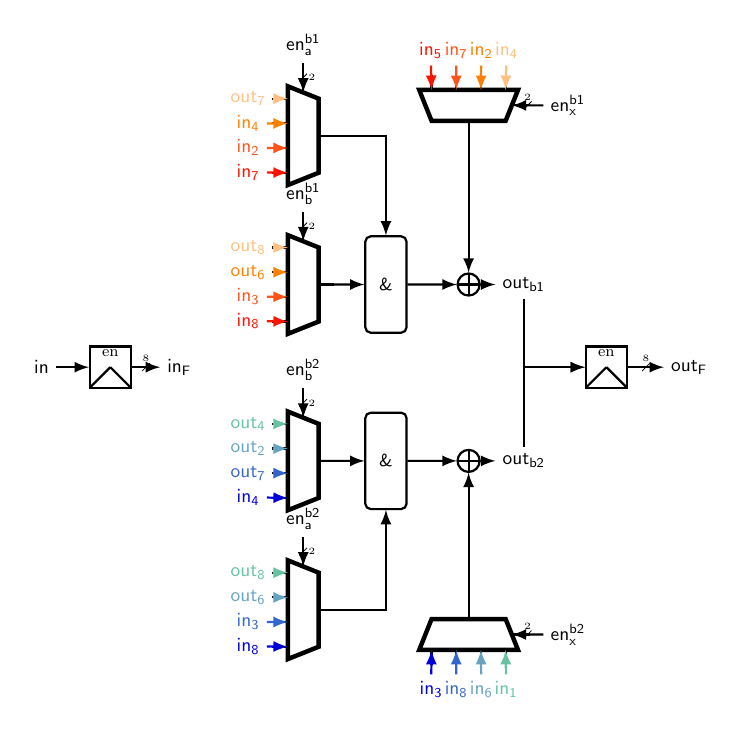
\begin{tikzpicture}[thick]% coordinates%\begin{}[]%\addplot coordinates {};%\end{}%\end{}
\begin{scope}[scale=.7, every node/.style={transform shape}]
  
  \begin{scope}[xshift = -6cm]
    \node [] (in) at (-.25, 0) {$\mathsf{in}$};
    \draw [] (1, 0) \registerEn{reg1};
    \node [] (inf) at (2.25, 0) {$\mathsf{in_{F}}$};
    \draw [-latex] (in) -- (reg1);
    \draw [-latex] (reg1) -- node {\bitwidth} node [bitwidth] {8} (inf);
\end{scope}
\begin{scope}[xshift = 3cm]
  \draw [] (1, 0) \registerEn{reg2};
  \node [] (outf) at (2.5, 0) {$\mathsf{out_{F}}$};
\end{scope}



  \begin{scope}[xshift = -1.5cm]
  
  \node [mux 4by2, thick, yscale=-.8](M1) at (0, 1.5){};
  \node [color = red!85!orange] (in1) at (-1, .84) {$\mathsf{in_8}$};
  \node [color = red!50!orange!90!white] (in2) at (-1, 1.28) {$\mathsf{in_3}$};
  \node [color = orange] (in3) at (-1, 1.72) {$\mathsf{out_6}$};
  \node [color = orange!50!white] (in4) at (-1, 2.17) {$\mathsf{out_8}$};
  \node [] (en1b) at (0, 3.15) {$\mathsf{en_b^{b1}}$};
  \draw [-latex] (en1b) -- node {\bitwidth} node [bitwidthvert] {2}(M1.bbpin 1);

  \draw [-latex, thick, color = red!85!orange] (in1) -- (M1.blpin 1);
  \draw [-latex, thick, color = red!50!orange!90!white] (in2) -- (M1.blpin 2);
  \draw [-latex, thick, color = orange] (in3) -- (M1.blpin 3);
  \draw [-latex, thick, color = orange!50!white] (in4) -- (M1.blpin 4);

\end{scope}

\begin{scope}[xshift = -1.5cm, yshift = 2.7cm]
  \node [mux 4by2, thick, yscale=-.8](M2) at (0, 1.5){};

  \node [color = red!85!orange] (in1) at (-1, .84) {$\mathsf{in_7}$};
  \node [color = red!50!orange!90!white] (in2) at (-1, 1.28) {$\mathsf{in_2}$};
  \node [color = orange] (in3) at (-1, 1.72) {$\mathsf{in_4}$};
  \node [color = orange!50!white] (in4) at (-1, 2.17) {$\mathsf{out_7}$};

  \node [] (en1a) at (0, 3.15) {$\mathsf{en_a^{b1}}$};
  \draw [-latex] (en1a) -- node {\bitwidth} node [bitwidthvert] {2} (M2.bbpin 1);
  \draw [-latex, thick, color = red!85!orange] (in1) -- (M2.blpin 1);
  \draw [-latex, thick, color = red!50!orange!90!white] (in2) -- (M2.blpin 2);
  \draw [-latex, thick, color = orange] (in3) -- (M2.blpin 3);
  \draw [-latex, thick, color = orange!50!white] (in4) -- (M2.blpin 4);
\end{scope}

\begin{scope}[xshift = 1.5cm, yshift = 3.25cm]
  \node [mux 4by2, thick, yscale=-1, xscale = .8, rotate = 90](M3) at (0, 1.5){};

  \node [color = red!85!orange] (in1) at (-.69, 2.5) {$\mathsf{in_5}$};
  \node [color = red!50!orange!90!white] (in2) at (-.225, 2.5) {$\mathsf{in_7}$};
  \node [color = orange] (in3) at (.23, 2.5) {$\mathsf{in_2}$};
  \node [color = orange!50!white] (in4) at (.69, 2.5) {$\mathsf{in_4}$};
  \node [] (en1x) at (1.8, 1.5) {$\mathsf{en_x^{b1}}$};
  \draw [-latex] (en1x) -- node {\bitwidth} node [bitwidth] {2} (M3.bbpin 1);

  \draw [-latex, thick, color = red!85!orange] (in1) -- (M3.blpin 1);
  \draw [-latex, thick, color = red!50!orange!90!white] (in2) -- (M3.blpin 2);
  \draw [-latex, thick, color = orange] (in3) -- (M3.blpin 3);
  \draw [-latex, thick, color = orange!50!white] (in4) -- (M3.blpin 4);
\end{scope}
\begin{scope}[xshift = 1.5cm, yshift = -6.35cm]
  \node [mux 4by2, thick, yscale=1, xscale = .8, rotate = 90](M4) at (0, 1.5){};


  \node [color = blue!85!black] (in1) at (-.68, .5) {$\mathsf{in_3}$};
  \node [color = blue!75!green!80!white] (in2) at (-.225, .5) {$\mathsf{in_8}$};
  \node [color = green!40!blue!60!white] (in3) at (.23, .5) {$\mathsf{in_6}$};
  \node [color = green!60!blue!60!white] (in4) at (.68, .5) {$\mathsf{in_1}$};

  \node [] (en1b) at (1.8, 1.5) {$\mathsf{en_x^{b2}}$};
  \draw [-latex] (en1b) -- node {\bitwidth} node [bitwidth] {2}(M4.bbpin 1);
  \draw [-latex, thick, color = blue!85!black] (in1) -- (M4.blpin 1);
  \draw [-latex, thick, color = blue!75!green!80!white] (in2) -- (M4.blpin 2);
  \draw [-latex, thick, color = green!40!blue!60!white] (in3) -- (M4.blpin 3);
  \draw [-latex, thick, color = green!60!blue!60!white] (in4) -- (M4.blpin 4);
\end{scope}
\begin{scope}[xshift = -1.5cm, yshift = -5.9cm]
  \node [mux 4by2, thick, yscale=-.8](M5) at (0, 1.5){};

  \node [color = blue!85!black] (in1) at (-1, .84) {$\mathsf{in_8}$};
  \node [color = blue!75!green!80!white] (in2) at (-1, 1.28) {$\mathsf{in_3}$};
  \node [color = green!40!blue!60!white] (in3) at (-1, 1.72) {$\mathsf{out_6}$};
  \node [color = green!60!blue!60!white] (in4) at (-1, 2.17) {$\mathsf{out_8}$};
  
  \node [] (en1b) at (0, 3.15) {$\mathsf{en_a^{b2}}$};
  \draw [-latex] (en1b) -- node {\bitwidth} node [bitwidthvert] {2}(M5.bbpin 1);
  \draw [-latex, thick, color = blue!85!black] (in1) -- (M5.blpin 1);
  \draw [-latex, thick, color = blue!75!green!80!white] (in2) -- (M5.blpin 2);
  \draw [-latex, thick, color = green!40!blue!60!white] (in3) -- (M5.blpin 3);
  \draw [-latex, thick, color = green!60!blue!60!white] (in4) -- (M5.blpin 4);
\end{scope}
\begin{scope}[xshift = -1.5cm, yshift = -3.2cm]
  \node [mux 4by2, thick, yscale=-.8](M6) at (0, 1.5){};

  \node [color = blue!85!black] (in1) at (-1, .84) {$\mathsf{in_4}$};
  \node [color = blue!75!green!80!white] (in2) at (-1, 1.28) {$\mathsf{out_7}$};
  \node [color = green!40!blue!60!white] (in3) at (-1, 1.72) {$\mathsf{out_2}$};
  \node [color = green!60!blue!60!white] (in4) at (-1, 2.17) {$\mathsf{out_4}$};
  
  \node [] (en1b) at (0, 3.15) {$\mathsf{en_b^{b2}}$};
  \draw [-latex] (en1b) -- node {\bitwidth} node [bitwidthvert] {2}(M6.bbpin 1);
  \draw [-latex, thick, color = blue!85!black] (in1) -- (M6.blpin 1);
  \draw [-latex, thick, color = blue!75!green!80!white] (in2) -- (M6.blpin 2);
  \draw [-latex, thick, color = green!40!blue!60!white] (in3) -- (M6.blpin 3);
  \draw [-latex, thick, color = green!60!blue!60!white] (in4) -- (M6.blpin 4);
\end{scope}
  \begin{scope}
  
  \node[rectangle,
  minimum width = .75cm,
  minimum height = 1.75cm,
  draw,
  rounded corners = 2pt
  ] (and1) at (0,1.5) {\small \textsf{\&}};

  \node[rectangle,
  minimum width = .75cm,
  minimum height = 1.75cm,
  draw,
  rounded corners = 2pt
  ] (and2) at (0,-1.7) {\small \textsf{\&}};

  \draw [] (1.5, 1.5) \xord{xor1};
  \draw [] (1.5, -1.7) \xord{xor2};
  \node [] (outb1) at (2.5, 1.5) {$\mathsf{out_{b1}}$};
  \node [] (outb2) at (2.5, -1.7) {$\mathsf{out_{b2}}$};
  
\end{scope}

\draw [-latex] (M1.brpin 1) -- (and1);
\draw [-latex] (M6.brpin 1) -- (and2);

\draw [-latex] (M2.brpin 1) -| (and1);
\draw [-latex] (M5.brpin 1) -| (and2);

\draw [-latex] (M3.brpin 1) -| (xor1);
\draw [-latex] (M4.brpin 1) -|  (xor2);

\draw [-latex] (and1) -- (xor1);
\draw [-latex] (and2) -- (xor2);

\draw [-latex] (xor1) -- (outb1);
\draw [-latex] (xor2) -- (outb2);

\draw [-latex] (outb1) |- (reg2);
\draw [-latex] (outb2) |- (reg2);
\draw [-latex] (reg2) -- node {\bitwidth} node [bitwidth] {8} (outf);

\end{scope}

\end{tikzpicture}
    \caption{%
        Architecture of low-latency masked Skinny Sbox.
    }
    \label{fig:sboxopt_circuit}
    \label{fig:sbox}
\end{figure}

Lastly, we discuss fully pipeline architectures.
While such architectures can achieve very high throughput that compensate for
their large area, they are difficult to use in our case.
Indeed, we are not interested in parallel Skinny evaluations (since this is not
useful for encrypting a single message with a Romulus-T leveled
implementation). Therefore, the latency
overhead of filling the pipeline (of at least 6~cycles) is significant when it
is used for only 16 Sbox evaluations (a Skinny round).
We however note that the only other HPC Skinny implementation we
know of uses that strategy, and uses a depth-12 pipeline~\cite{khairallahhardware}.\footnote{%
    Which can be improved to depth-6 thanks to the asymmetric
    latency of HPC2 ANDs.
}

\subsubsection{Skinny.}\label{subsub:skinny}

Based on these Sbox architectures, we design three Skinny implementations with
various area vs. latency trade-offs.
The two first ones are simple round-based architectures, as shown in
\autoref{fig:skinny8}, where either 16~low-latency Sboxes (``low-latency
Skinny'', \skinnyll) or 8~high-throughput (``balanced Skinny'', \skinnyb)
Sboxes are used.
The third implementation (``small Skinny'', \skinnys) targets lower area: it is
a serialized architecture that instantiates only one high-throughput Sbox (that
is used 8~times per round), as shown in \autoref{fig:skinny1}.

\begin{figure}
    \centering
    \resizebox{.9\textwidth}{!}{


%% Document
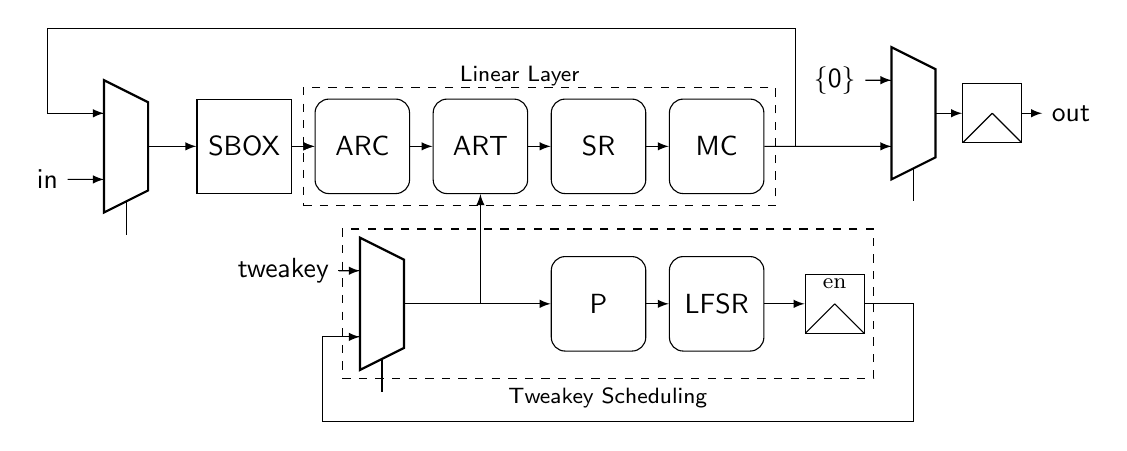
\begin{tikzpicture}[
]
\node [] (i) at (-1, -.42) {$\mathsf{in}$};
\node [] (o) at (12, .42) {$\mathsf{out}$};
\node [] (zero) at (9, .84) {$\mathsf{\{0\}}$};
\node [] (tk) at (2, -1.58) {$\mathsf{tweakey}$};

\node [mux 2by2, rotate = 0](M1) at (0, 0){};
\node [mux 2by2, rotate = 0](M2) at (10, 0.42){};
\node [mux 2by2, rotate = 0](M3) at (3.25, -2){};

\node[rectangle,
minimum width = 1.2cm,
minimum height = 1.2cm,
draw] (B1) at (1.5,0) {\textsf{SBOX}};

\node[rectangle,
minimum width = 1.2cm,
minimum height = 1.2cm,
rounded corners = 5pt,
draw] (arc) at (3,0) {\textsf{ARC}};


\node[rectangle,
minimum width = 1.2cm,
rounded corners = 5pt, 
minimum height = 1.2cm,
draw] (art) at (4.5,0) {\textsf{ART}};
\node [] (ll) at (5, .9) {\footnotesize\textsf{Linear Layer}};

\node[rectangle,
dashed,
minimum width = 6cm,
minimum height = 1.5cm,
draw] (sr) at (5.25,0) {};

\node[rectangle,
minimum width = 1.2cm,
rounded corners = 5pt, 
minimum height = 1.2cm,
draw] (sr) at (6,0) {\textsf{SR}};

\node[rectangle,
minimum width = 1.2cm,
rounded corners = 5pt, 
minimum height = 1.2cm,
draw] (mc) at (7.5,0) {\textsf{MC}};

\node[rectangle,
minimum width = 1.2cm,
rounded corners = 5pt, 
minimum height = 1.2cm,
draw] (P) at (6, -2) {\textsf{P}};

\node[rectangle,
minimum width = 1.2cm,
rounded corners = 5pt, 
minimum height = 1.2cm,
draw] (LFSR) at (7.5,-2) { \textsf{LFSR}};

\draw [] (9, -2) \registerEn{reg1};
\draw [] (11, .42) \register{rego};



\draw [-latex] (B1) -- (arc);
\draw [-latex] (arc) -- (art);
\draw [-latex] (art) -- (sr);
\draw [-latex] (sr) -- (mc);
\draw [-latex] (B1) -- (arc);
\draw [-latex] (mc) -- (M2.blpin 2);
\draw [-latex] (M1.brpin 1) -- (B1);
\draw [] (8.5, 0) |- (-1,1.5);
\draw [-latex] (i) -- (M1.blpin 2);

\draw [-latex] (-1, 1.5) |- (M1.blpin 1);
\draw [-latex] (M2.brpin 1) -- (rego);
\draw [-latex] (rego) -- (o);

\draw [-latex] (M3.brpin 1) -- (P);
\draw [-latex] (P) -- (LFSR);
\draw [-latex] (4.5,-2) -- (art);
\draw [-latex] (LFSR) -- (reg1);

\draw [] (reg1) -- (10, -2);

\draw [] (10, -2) |- (2.5, -3.5);
\draw [-latex] (2.5, -3.5) |- (M3.blpin 2);
\draw [-latex] (tk) -- (M3.blpin 1);

\node[rectangle,
dashed,
minimum width = 6.75cm,
minimum height = 1.9cm,
draw] (sr) at (6.12,-2) {};
\node [] (ll) at (6.12, -3.2) {\footnotesize\textsf{Tweakey Scheduling}};
\draw [-latex] (zero) -- (M2.blpin 1);

\end{tikzpicture}}
    \caption{Round-based masked Skinny architecture (\skinnyll and \skinnyb).}
    \label{fig:skinny8}
\end{figure}

\begin{figure}
    \centering
    \resizebox{.9\textwidth}{!}{


%% Document
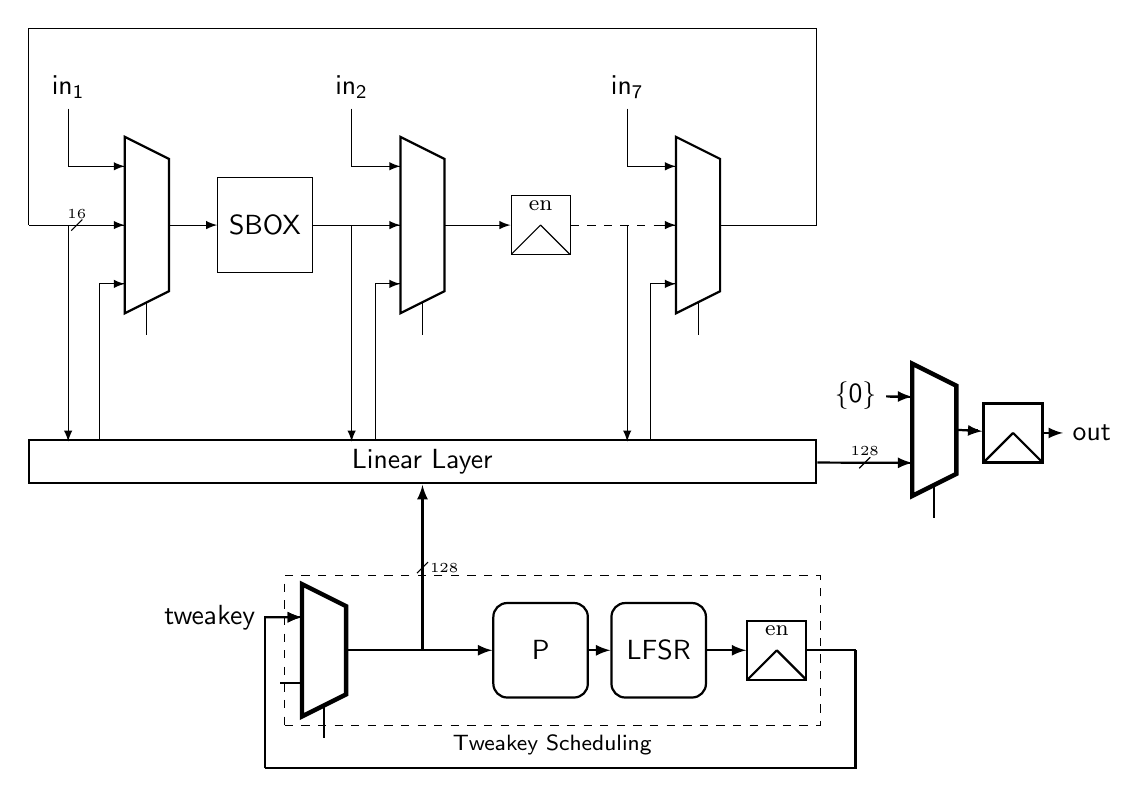
\begin{tikzpicture}[
]
\node [] (i1) at (-1, 1.75) {$\mathsf{in_1}$};
\node [] (i2) at (2.6, 1.75) {$\mathsf{in_2}$};
\node [] (i3) at (6.1, 1.75) {$\mathsf{in_7}$};

\node [mux 3by2, rotate = 0](M1) at (0, 0){};
\node [mux 3by2, rotate = 0](M3) at (3.5, 0){};
\node [mux 3by2, rotate = 0](M2) at (7, 0){};
\node [mux 2by2, rotate = 0, thick](Mo) at (10, -2.6){};


\draw [] (5, 0) \registerEn{reg1};

\node[rectangle,
minimum width = 1.2cm,
minimum height = 1.2cm,
draw] (B1) at (1.5,0) {\textsf{SBOX}};


\node[rectangle,
thick,
minimum width = 10cm,
minimum height = .4cm,
draw] (ll) at (3.5, -3) {\textsf{Linear Layer}};

\draw [-latex] (-1.5,0) -- node {\bitwidth} node [bitwidth] {16} (M1.blpin 2);

\draw [] (M2.brpin 1) -| (8.5, 2.5);
\draw [] (8.5, 2.5) -| (-1.5, 0);
\draw [thick, -latex] (ll) -- node {\bitwidth} node [bitwidth] {128} (Mo.blpin 2);

\draw [-latex] (-1,0) -- (-1, -2.75);
\draw [-latex] (2.6,0) -- (2.6, -2.75);
\draw [-latex] (6.1,0) -- (6.1, -2.75);

\draw [-latex] (-.6,-2.73) |- (M1.blpin 3);
\draw [-latex] (2.9,-2.73) |- (M3.blpin 3);
\draw [-latex] (6.4 ,-2.73) |- (M2.blpin 3);



\draw [-latex] (M1.brpin 1) -- (B1);
\draw [-latex] (B1) -- (M3.blpin 2);
\draw [-latex] (M3.brpin 1) -- (reg1);



\draw [-latex] (i1) |-  (M1.blpin 1);
\draw [-latex] (i2) |- (M3.blpin 1);
\draw [-latex] (i3) |- (M2.blpin 1);

\draw [-latex, dashed] (reg1) -- (M2.blpin 2);


\begin{scope}[yshift = -3.4cm, xshift = -1 cm]
    \node [] (tk) at (1.8, -1.58) {$\mathsf{tweakey}$};
    \draw [thick] (9, -2) \registerEn{reg2};
    \draw [thick] (12, .76) \register{reg3};

    \node [] (o) at (13, .76) {$\mathsf{out}$};
    \node [] (zero) at (10, 1.23) {$\mathsf{\{0\}}$};

    \node [mux 2by2, rotate = 0, thick](M3) at (3.25, -2){};

    \node[rectangle,
    minimum width = 1.2cm,
    minimum height = 1.2cm,
    rounded corners = 5pt,
    thick,
    draw] (P) at (6, -2) {\textsf{P}};

    \node[rectangle,
    minimum width = 1.2cm,
    minimum height = 1.2cm,
    thick,
    rounded corners = 5pt,
    draw] (LFSR) at (7.5,-2) { \textsf{LFSR}};

    \draw [-latex, thick] (M3.brpin 1) -- (P);
    \draw [-latex, thick] (P) -- (LFSR);
    \draw [-latex, thick] (4.5,-2) -- node {\bitwidth} node [bitwidthvert] {128}(4.5, 0.1);
    \draw [-latex, thick] (LFSR) -- (reg2);

    \draw [thick] (reg2) -- (10, -2);
    \draw [thick] (10,-2) |- (2.5, -3.5);
    \draw [-latex, thick] (2.5, -3.5) |- (M3.blpin 1);
    \draw [-latex, thick] (tk) -- (M3.blpin 1);
    \draw [-latex, thick] (zero) -- (Mo.blpin 1);
    \draw [-latex, thick] (reg3) -- (o);
    \draw [-latex, thick] (Mo.brpin 1) -- (reg3);

    \node[rectangle,
    dashed,
    minimum width = 6.8cm,
    minimum height = 1.9cm,
    draw] (sr) at (6.15,-2) {};
    \node [] (ll) at (6.15, -3.2) {\footnotesize\textsf{Tweakey Scheduling}};


\end{scope}

\end{tikzpicture}}
    \caption{Serialized masked Skinny architecture (\skinnys).}
    \label{fig:skinny1}
\end{figure}

Let us now discuss the performance of these implementations.
We consider latency, randomness requirements and area as performance metrics,
since the critical path
will be similar in all cases (it lies in the linear layer).
The latency and maximum randomness requirements per cycle
of the implementations are shown in \autoref{tab:latencyrandomness}.
%\footnote{%
%    This randomness figure characterizes the number of randomness generators
%    needed if no randomness is stored.
%}
We can see that the \skinnys implementation has 8~times the latency of \skinnyb (due to 8x
serialization), while \skinnyll reduces latency by 33~\% compared to \skinnyb.
Regarding randomness, the maximum randomness throughput of \skinnys is 8~times
lower than \skinnyb, and the one of \skinnyll is twice the one of \skinnyb.

\begin{table}
    \centering
    \setlength\tabcolsep{0.4em}
    \begin{tabular}{lcccccc}
        \toprule
       & \multirow{2}{*}{Latency [cycle]} & \multicolumn{5}{c}{Randomness [bit]} \\
       &                          & $d = 2$ & $d=3$   & $d = 4$ & $d=5$   & $d = 6$    \\
       \midrule
        \skinnys  & 2880                     & 2  & 6      & 12   & 20     & 30       \\
        \skinnyb  & 360                      & 16   & 48    & 96 & 160       & 240      \\
        \skinnyll & 240                      & 32       & 96   & 192    & 320  & 480    \\
    \bottomrule
    \end{tabular}
    \vspace*{3ex}
    \caption{
        Skinny-384+ masked implementations: total latency and maximum randomness
        consumption for a single clock cycle (where the total randomness consumption
        is $64 \cdot d \cdot (d-1)$ bits for all three implementations).
    }
    \label{tab:latencyrandomness}
\end{table}

Next, we look at area requirements in \autoref{fig:primarea}.
The Sbox logic area clearly reflects the architectural choices: 2 AND and XOR
gadgets for \skinnys, 16 of each for \skinnyb, and 32 of each for \skinnyll.
Next, the remaining Sbox area is fairly high for \skinnyll due to the large
number of Sbox instances and due to their large MUXes and registers.
For \skinnyb and \skinnys, the larger number MUXes and registers in the Sboxes
of the former compensate for the more complex datapath of the latter, resulting
in a similar ``routing'' area for both of them.
The remaining parts of Skinny are the same for all three architectures.
Overall, the difference in area between the architectures is small for low
number of shares, and increases as the latter grows.
For all considered number of shares ($d \le 6$), the Sboxes do not dominate the
area of neither \skinnys nor \skinnyb, hence \skinnys brings a limited area
gain at a large latency cost compared to \skinnyb.
On the other hand, \skinnyll has an area overhead of up to 39~\% (for $d\le 6$),
and a latency gain of 33~\% over \skinnyb.
\begin{figure}
	\centering
	% This file was created with tikzplotlib v0.9.17.
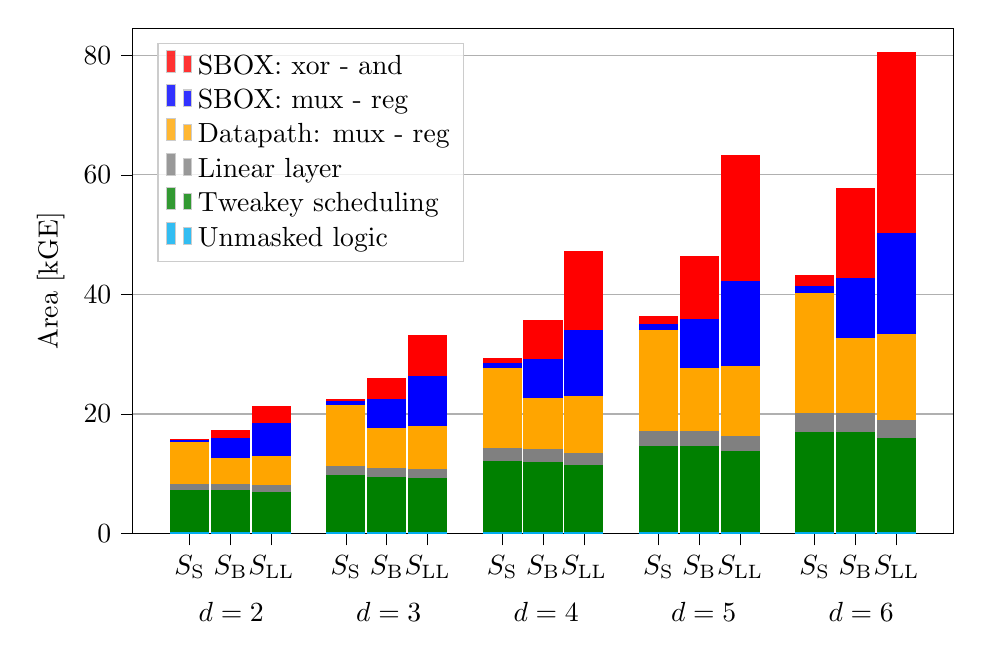
\begin{tikzpicture}
\definecolor{color0}{rgb}{1,0.647058823529412,0}

\node [] (d2) at (1.25, -1) { $d = 2$};
\node [] (d3) at (3.25, -1) { $d = 3$};
\node [] (d4) at (5.25, -1) { $d = 4$};
\node [] (d5) at (7.25, -1) { $d = 5$};
\node [] (d6) at (9.25, -1) { $d = 6$};

\begin{axis}[
height=8cm,
legend cell align={left},
legend style={
  fill opacity=0.8,
  draw opacity=1,
  text opacity=1,
  at={(0.03,0.97)},
  anchor=north west,
  draw=white!80!black
},
tick align=outside,
tick pos=left,
width=12cm,
x grid style={white!69.0196078431373!black},
xmin=1.375125, xmax=6.624875,
xtick style={color=black},
xtick={1.73875,2,2.26125,2.73875,3,3.26125,3.73875,4,4.26125,4.73875,5,5.26125,5.73875,6,6.26125},
xticklabel style={rotate=0},
xticklabels={
  \skinnys,
  \skinnyb,
  \skinnyll,
  \skinnys,
  \skinnyb,
  \skinnyll,
  \skinnys,
  \skinnyb,
  \skinnyll,
  \skinnys,
  \skinnyb,
  \skinnyll,
  \skinnys,
  \skinnyb,
  \skinnyll,
},
y grid style={white!69.0196078431373!black},
ylabel={Area [kGE]},
ymajorgrids,
ymin=0, ymax=84.5137515,
ytick style={color=black}
]
\draw[draw=none,fill=cyan] (axis cs:1.61375,0) rectangle (axis cs:1.86375,0.2166);

\addlegendimage{ybar,ybar legend,draw=none,fill=red}
\addlegendentry{SBOX: xor - and}

\addlegendimage{ybar,ybar legend,draw=none,fill=blue}
\addlegendentry{SBOX: mux - reg}

\addlegendimage{ybar,ybar legend,draw=none,fill=color0}
\addlegendentry{Datapath: mux - reg}

\addlegendimage{ybar,ybar legend,draw=none,fill=white!50.1960784313725!black}
\addlegendentry{Linear layer}

\addlegendimage{ybar,ybar legend,draw=none,fill=green!50.1960784313725!black}
\addlegendentry{Tweakey scheduling}

\addlegendimage{ybar,ybar legend,draw=none,fill=cyan}
\addlegendentry{Unmasked logic}

\draw[draw=none,fill=cyan] (axis cs:1.875,0) rectangle (axis cs:2.125,0.2166);
\draw[draw=none,fill=cyan] (axis cs:2.13625,0) rectangle (axis cs:2.38625,0.2166);
\draw[draw=none,fill=cyan] (axis cs:2.61375,0) rectangle (axis cs:2.86375,0.2166);
\draw[draw=none,fill=cyan] (axis cs:2.875,0) rectangle (axis cs:3.125,0.2166);
\draw[draw=none,fill=cyan] (axis cs:3.13625,0) rectangle (axis cs:3.38625,0.2166);
\draw[draw=none,fill=cyan] (axis cs:3.61375,0) rectangle (axis cs:3.86375,0.2166);
\draw[draw=none,fill=cyan] (axis cs:3.875,0) rectangle (axis cs:4.125,0.2166);
\draw[draw=none,fill=cyan] (axis cs:4.13625,0) rectangle (axis cs:4.38625,0.2166);
\draw[draw=none,fill=cyan] (axis cs:4.61375,0) rectangle (axis cs:4.86375,0.2166);
\draw[draw=none,fill=cyan] (axis cs:4.875,0) rectangle (axis cs:5.125,0.2166);
\draw[draw=none,fill=cyan] (axis cs:5.13625,0) rectangle (axis cs:5.38625,0.2166);
\draw[draw=none,fill=cyan] (axis cs:5.61375,0) rectangle (axis cs:5.86375,0.2166);
\draw[draw=none,fill=cyan] (axis cs:5.875,0) rectangle (axis cs:6.125,0.2166);
\draw[draw=none,fill=cyan] (axis cs:6.13625,0) rectangle (axis cs:6.38625,0.2166);
\draw[draw=none,fill=green!50.1960784313725!black] (axis cs:1.61375,0.2166) rectangle (axis cs:1.86375,7.27386928571429);

\draw[draw=none,fill=green!50.1960784313725!black] (axis cs:1.875,0.2166) rectangle (axis cs:2.125,7.26846714285714);
\draw[draw=none,fill=green!50.1960784313725!black] (axis cs:2.13625,0.2166) rectangle (axis cs:2.38625,6.99350714285714);
\draw[draw=none,fill=green!50.1960784313725!black] (axis cs:2.61375,0.2166) rectangle (axis cs:2.86375,9.76796928571429);
\draw[draw=none,fill=green!50.1960784313725!black] (axis cs:2.875,0.2166) rectangle (axis cs:3.125,9.41060357142857);
\draw[draw=none,fill=green!50.1960784313725!black] (axis cs:3.13625,0.2166) rectangle (axis cs:3.38625,9.26035142857143);
\draw[draw=none,fill=green!50.1960784313725!black] (axis cs:3.61375,0.2166) rectangle (axis cs:3.86375,12.1753628571429);
\draw[draw=none,fill=green!50.1960784313725!black] (axis cs:3.875,0.2166) rectangle (axis cs:4.125,12.0006871428571);
\draw[draw=none,fill=green!50.1960784313725!black] (axis cs:4.13625,0.2166) rectangle (axis cs:4.38625,11.4622757142857);
\draw[draw=none,fill=green!50.1960784313725!black] (axis cs:4.61375,0.2166) rectangle (axis cs:4.86375,14.5965478571429);
\draw[draw=none,fill=green!50.1960784313725!black] (axis cs:4.875,0.2166) rectangle (axis cs:5.125,14.5965478571429);
\draw[draw=none,fill=green!50.1960784313725!black] (axis cs:5.13625,0.2166) rectangle (axis cs:5.38625,13.81624);
\draw[draw=none,fill=green!50.1960784313725!black] (axis cs:5.61375,0.2166) rectangle (axis cs:5.86375,17.0075435714286);
\draw[draw=none,fill=green!50.1960784313725!black] (axis cs:5.875,0.2166) rectangle (axis cs:6.125,17.0075435714286);
\draw[draw=none,fill=green!50.1960784313725!black] (axis cs:6.13625,0.2166) rectangle (axis cs:6.38625,15.9515421428571);
\draw[draw=none,fill=white!50.1960784313725!black] (axis cs:1.61375,7.27386928571429) rectangle (axis cs:1.86375,8.33765214285714);

\draw[draw=none,fill=white!50.1960784313725!black] (axis cs:1.875,7.26846714285714) rectangle (axis cs:2.125,8.33225);
\draw[draw=none,fill=white!50.1960784313725!black] (axis cs:2.13625,6.99350714285714) rectangle (axis cs:2.38625,8.05729);
\draw[draw=none,fill=white!50.1960784313725!black] (axis cs:2.61375,9.76796928571429) rectangle (axis cs:2.86375,11.3384907142857);
\draw[draw=none,fill=white!50.1960784313725!black] (axis cs:2.875,9.41060357142857) rectangle (axis cs:3.125,10.981125);
\draw[draw=none,fill=white!50.1960784313725!black] (axis cs:3.13625,9.26035142857143) rectangle (axis cs:3.38625,10.8308728571429);
\draw[draw=none,fill=white!50.1960784313725!black] (axis cs:3.61375,12.1753628571429) rectangle (axis cs:3.86375,14.2526228571429);
\draw[draw=none,fill=white!50.1960784313725!black] (axis cs:3.875,12.0006871428571) rectangle (axis cs:4.125,14.0779471428571);
\draw[draw=none,fill=white!50.1960784313725!black] (axis cs:4.13625,11.4622757142857) rectangle (axis cs:4.38625,13.5395357142857);
\draw[draw=none,fill=white!50.1960784313725!black] (axis cs:4.61375,14.5965478571429) rectangle (axis cs:4.86375,17.1805457142857);
\draw[draw=none,fill=white!50.1960784313725!black] (axis cs:4.875,14.5965478571429) rectangle (axis cs:5.125,17.1805457142857);
\draw[draw=none,fill=white!50.1960784313725!black] (axis cs:5.13625,13.81624) rectangle (axis cs:5.38625,16.4002378571429);
\draw[draw=none,fill=white!50.1960784313725!black] (axis cs:5.61375,17.0075435714286) rectangle (axis cs:5.86375,20.09828);
\draw[draw=none,fill=white!50.1960784313725!black] (axis cs:5.875,17.0075435714286) rectangle (axis cs:6.125,20.09828);
\draw[draw=none,fill=white!50.1960784313725!black] (axis cs:6.13625,15.9515421428571) rectangle (axis cs:6.38625,19.0422785714286);
\draw[draw=none,fill=color0] (axis cs:1.61375,8.33765214285714) rectangle (axis cs:1.86375,15.2929971428571);

\draw[draw=none,fill=color0] (axis cs:1.875,8.33225) rectangle (axis cs:2.125,12.6442278571429);
\draw[draw=none,fill=color0] (axis cs:2.13625,8.05729) rectangle (axis cs:2.38625,13.0211614285714);
\draw[draw=none,fill=color0] (axis cs:2.61375,11.3384907142857) rectangle (axis cs:2.86375,21.5081285714286);
\draw[draw=none,fill=color0] (axis cs:2.875,10.981125) rectangle (axis cs:3.125,17.6026285714286);
\draw[draw=none,fill=color0] (axis cs:3.13625,10.8308728571429) rectangle (axis cs:3.38625,17.987565);
\draw[draw=none,fill=color0] (axis cs:3.61375,14.2526228571429) rectangle (axis cs:3.86375,27.731505);
\draw[draw=none,fill=color0] (axis cs:3.875,14.0779471428571) rectangle (axis cs:4.125,22.616465);
\draw[draw=none,fill=color0] (axis cs:4.13625,13.5395357142857) rectangle (axis cs:4.38625,23.0396728571429);
\draw[draw=none,fill=color0] (axis cs:4.61375,17.1805457142857) rectangle (axis cs:4.86375,33.968275);
\draw[draw=none,fill=color0] (axis cs:4.875,17.1805457142857) rectangle (axis cs:5.125,27.6558871428571);
\draw[draw=none,fill=color0] (axis cs:5.13625,16.4002378571429) rectangle (axis cs:5.38625,28.0685471428571);
\draw[draw=none,fill=color0] (axis cs:5.61375,20.09828) rectangle (axis cs:5.86375,40.190405);
\draw[draw=none,fill=color0] (axis cs:5.875,20.09828) rectangle (axis cs:6.125,32.7631778571428);
\draw[draw=none,fill=color0] (axis cs:6.13625,19.0422785714286) rectangle (axis cs:6.38625,33.3141728571429);
\draw[draw=none,fill=blue] (axis cs:1.61375,15.2929971428571) rectangle (axis cs:1.86375,15.7044257142857);

\draw[draw=none,fill=blue] (axis cs:1.875,12.6442278571429) rectangle (axis cs:2.125,15.9518564285714);
\draw[draw=none,fill=blue] (axis cs:2.13625,13.0211614285714) rectangle (axis cs:2.38625,18.5518757142857);
\draw[draw=none,fill=blue] (axis cs:2.61375,21.5081285714286) rectangle (axis cs:2.86375,22.1263);
\draw[draw=none,fill=blue] (axis cs:2.875,17.6026285714286) rectangle (axis cs:3.125,22.5665142857143);
\draw[draw=none,fill=blue] (axis cs:3.13625,17.987565) rectangle (axis cs:3.38625,26.2839364285714);
\draw[draw=none,fill=blue] (axis cs:3.61375,27.731505) rectangle (axis cs:3.86375,28.555905);
\draw[draw=none,fill=blue] (axis cs:3.875,22.616465) rectangle (axis cs:4.125,29.2363507142857);
\draw[draw=none,fill=blue] (axis cs:4.13625,23.0396728571429) rectangle (axis cs:4.38625,34.10153);
\draw[draw=none,fill=blue] (axis cs:4.61375,33.968275) rectangle (axis cs:4.86375,34.9989035714286);
\draw[draw=none,fill=blue] (axis cs:4.875,27.6558871428571) rectangle (axis cs:5.125,35.9315157142857);
\draw[draw=none,fill=blue] (axis cs:5.13625,28.0685471428571) rectangle (axis cs:5.38625,42.2296742857143);
\draw[draw=none,fill=blue] (axis cs:5.61375,40.190405) rectangle (axis cs:5.86375,41.4272621428571);
\draw[draw=none,fill=blue] (axis cs:5.875,32.7631778571428) rectangle (axis cs:6.125,42.6948064285714);
\draw[draw=none,fill=blue] (axis cs:6.13625,33.3141728571429) rectangle (axis cs:6.38625,50.31331);
\draw[draw=none,fill=red] (axis cs:1.61375,15.7044257142857) rectangle (axis cs:1.86375,15.87812);

\draw[draw=none,fill=red] (axis cs:1.875,15.9518564285714) rectangle (axis cs:2.125,17.3414107142857);
\draw[draw=none,fill=red] (axis cs:2.13625,18.5518757142857) rectangle (axis cs:2.38625,21.3309842857143);
\draw[draw=none,fill=red] (axis cs:2.61375,22.1263) rectangle (axis cs:2.86375,22.5608628571429);
\draw[draw=none,fill=red] (axis cs:2.875,22.5665142857143) rectangle (axis cs:3.125,26.0430171428571);
\draw[draw=none,fill=red] (axis cs:3.13625,26.2839364285714) rectangle (axis cs:3.38625,33.2369421428571);
\draw[draw=none,fill=red] (axis cs:3.61375,28.555905) rectangle (axis cs:3.86375,29.3749507142857);
\draw[draw=none,fill=red] (axis cs:3.875,29.2363507142857) rectangle (axis cs:4.125,35.7887164285714);
\draw[draw=none,fill=red] (axis cs:4.13625,34.10153) rectangle (axis cs:4.38625,47.2062614285714);
\draw[draw=none,fill=red] (axis cs:4.61375,34.9989035714286) rectangle (axis cs:4.86375,36.3127478571429);
\draw[draw=none,fill=red] (axis cs:4.875,35.9315157142857) rectangle (axis cs:5.125,46.44227);
\draw[draw=none,fill=red] (axis cs:5.13625,42.2296742857143) rectangle (axis cs:5.38625,63.2511828571429);
\draw[draw=none,fill=red] (axis cs:5.61375,41.4272621428571) rectangle (axis cs:5.86375,43.322925);
\draw[draw=none,fill=red] (axis cs:5.875,42.6948064285714) rectangle (axis cs:6.125,57.7911378571429);
\draw[draw=none,fill=red] (axis cs:6.13625,50.31331) rectangle (axis cs:6.38625,80.4892871428571);
\end{axis}

\end{tikzpicture}

        \caption{
            Area requirements for the three masked Skinny hardware implementations in a
            \SI{65}{nm} ASIC technology using the HPC2 masking scheme.
        }
        \label{fig:primarea}\vspace*{-1cm}
\end{figure}

\subsection{Implementation of the modes}\label{subsec:modes}



We implemented side-channel protected hardware accelerators for
Romulus-N, Romulus-T, Ascon and ISAP, using the primitives described
in \autoref{tab:prim_latency}.
The Romulus-N implementation is fully masked and uses one
\skinnyll instance.
Next, the implementation of Romulus-T is leveled 
with one masked instance of Skinny (we also used \skinnyll) and four non-masked
Skinny instances (with a round-based architecture).
Similarly, the Ascon implementation is also leveled.
The masked \asconp primitive is based on the HPC2 masking scheme and is
serialized with 16 Sbox instances (each Sbox is a 2-stage pipeline 
performing 4~Sbox evaluations per round)\footnote{%
    This choice is somewhat arbitrary: we took a serialization factor that gives a good
    latency versus area trade-off.
    It also happens to lead to a latency of 6 clock cycles per round, which is
    the same latency as a round of \skinnyll.
},
while the non-masked permutation is round-based (1~cycle per round).
Finally, ISAP uses two instances of the non-masked \asconp primitive.

\begin{table}
    \centering
    \setlength\tabcolsep{0.4em}
    \begin{tabular}{lcccc}
        \toprule
    & \multicolumn{2}{c}{Masked}          & \multicolumn{2}{c}{Non-masked}          \\
    & Latency & Architecture & Latency & Architecture \\
    \midrule
        Skinny-384+  & 240 & \skinnyll          & 40  & round-based             \\
        $\asconp^{6}$  & &                & 6  & round-based              \\
        $\asconp^{12}$ & 72  & serialized 4x           & 12 & round-based              \\
        ISAP RK  &              &  & 152 & round-based \\ \bottomrule
    \end{tabular}
    \vspace*{3ex}
    \caption{
        Primitive implementations used in the AEAD cores: latency
        in clock cycles and architecture for masked and non-masked versions.
    }
    \label{tab:prim_latency}
\end{table}

Let us first discuss the latency of these implementations with
\autoref{fig:modelatency}.
The encryption time of Romulus-N grows very quickly with the message size due
to the need of masking all Skinny calls, which are slow compared to non-masked
calls (as shown in \autoref{tab:prim_latency}).
However, for very short messages, Romulus-N is fairly competitive thanks to its
low number of Skinny calls it that case.
On the other hand, Romulus-T has a larger upfront cost, due to the larger
number of Skinny calls even for short messages, however the mode-level leakage resistance
allows to use non-masked calls for the bulk processing, resulting in
lower latency than Romulus-N for long messages.
Next, Ascon enjoys lower initial latency and long-message latency than Romulus-T.
This is due to the lower number of rounds in $\asconp^{6}$ and $\asconp^{12}$ compared to
Skinny (which has 40 rounds).
Finally, the latency of ISAP is between the one of Ascon and Romulus-T.
Indeed, ISAP's bulk processing is very similar to Ascon's, but uses more rounds
to increase the security margin in presence of leakage.
Moreover, the leakage-resilient PRF of ISAP uses many permutation rounds, which
makes it slower than a masked Ascon for short messages, while still being
faster than Romulus-T.

\begin{figure}
    \centering
    % This file was created with tikzplotlib v0.9.17.
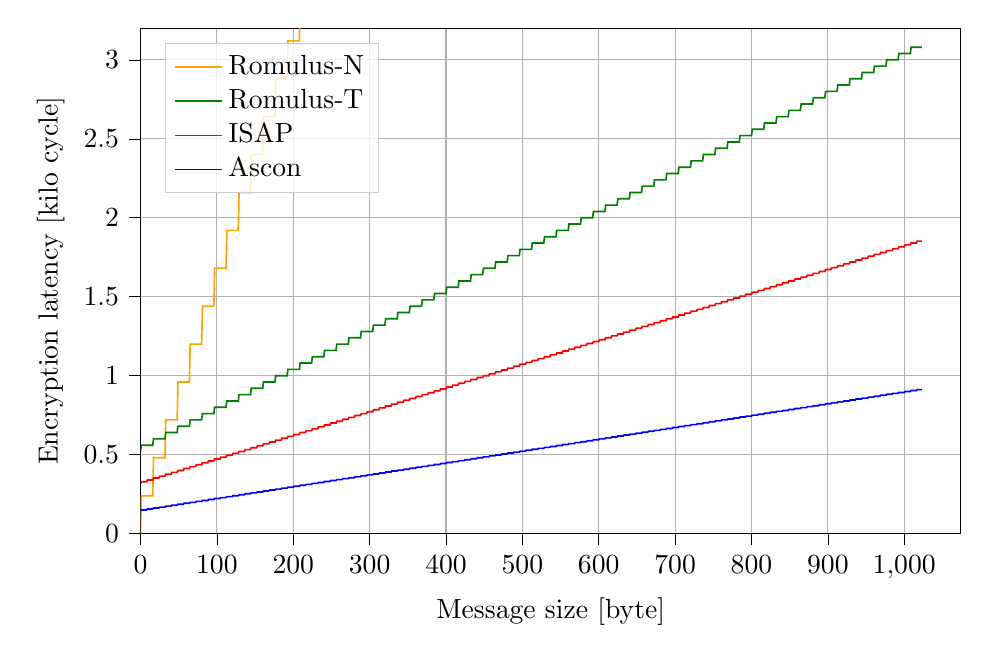
\begin{tikzpicture}

\definecolor{color0}{rgb}{1,0.647058823529412,0}

\begin{axis}[
height=8cm,
legend cell align={left},
legend style={
  fill opacity=0.8,
  draw opacity=1,
  text opacity=1,
  at={(0.03,0.97)},
  anchor=north west,
  draw=white!80!black
},
tick align=outside,
tick pos=left,
width=12cm,
x grid style={white!69.0196078431373!black},
xlabel={Message size [byte]},
xmajorgrids,
xmin=0, xmax=1074.15,
xtick style={color=black},
y grid style={white!69.0196078431373!black},
ylabel={Encryption latency [kilo cycle]},
ymajorgrids,
ymin=0, ymax=3.2,
ytick style={color=black}
]
\addplot [semithick, color0]
table {%
0 0
1 0.24
2 0.24
3 0.24
4 0.24
5 0.24
6 0.24
7 0.24
8 0.24
9 0.24
10 0.24
11 0.24
12 0.24
13 0.24
14 0.24
15 0.24
16 0.24
17 0.48
18 0.48
19 0.48
20 0.48
21 0.48
22 0.48
23 0.48
24 0.48
25 0.48
26 0.48
27 0.48
28 0.48
29 0.48
30 0.48
31 0.48
32 0.48
33 0.72
34 0.72
35 0.72
36 0.72
37 0.72
38 0.72
39 0.72
40 0.72
41 0.72
42 0.72
43 0.72
44 0.72
45 0.72
46 0.72
47 0.72
48 0.72
49 0.96
50 0.96
51 0.96
52 0.96
53 0.96
54 0.96
55 0.96
56 0.96
57 0.96
58 0.96
59 0.96
60 0.96
61 0.96
62 0.96
63 0.96
64 0.96
65 1.2
66 1.2
67 1.2
68 1.2
69 1.2
70 1.2
71 1.2
72 1.2
73 1.2
74 1.2
75 1.2
76 1.2
77 1.2
78 1.2
79 1.2
80 1.2
81 1.44
82 1.44
83 1.44
84 1.44
85 1.44
86 1.44
87 1.44
88 1.44
89 1.44
90 1.44
91 1.44
92 1.44
93 1.44
94 1.44
95 1.44
96 1.44
97 1.68
98 1.68
99 1.68
100 1.68
101 1.68
102 1.68
103 1.68
104 1.68
105 1.68
106 1.68
107 1.68
108 1.68
109 1.68
110 1.68
111 1.68
112 1.68
113 1.92
114 1.92
115 1.92
116 1.92
117 1.92
118 1.92
119 1.92
120 1.92
121 1.92
122 1.92
123 1.92
124 1.92
125 1.92
126 1.92
127 1.92
128 1.92
129 2.16
130 2.16
131 2.16
132 2.16
133 2.16
134 2.16
135 2.16
136 2.16
137 2.16
138 2.16
139 2.16
140 2.16
141 2.16
142 2.16
143 2.16
144 2.16
145 2.4
146 2.4
147 2.4
148 2.4
149 2.4
150 2.4
151 2.4
152 2.4
153 2.4
154 2.4
155 2.4
156 2.4
157 2.4
158 2.4
159 2.4
160 2.4
161 2.64
162 2.64
163 2.64
164 2.64
165 2.64
166 2.64
167 2.64
168 2.64
169 2.64
170 2.64
171 2.64
172 2.64
173 2.64
174 2.64
175 2.64
176 2.64
177 2.88
178 2.88
179 2.88
180 2.88
181 2.88
182 2.88
183 2.88
184 2.88
185 2.88
186 2.88
187 2.88
188 2.88
189 2.88
190 2.88
191 2.88
192 2.88
193 3.12
194 3.12
195 3.12
196 3.12
197 3.12
198 3.12
199 3.12
200 3.12
201 3.12
202 3.12
203 3.12
204 3.12
205 3.12
206 3.12
207 3.12
208 3.12
209 3.36
210 3.36
211 3.36
212 3.36
213 3.36
214 3.36
215 3.36
216 3.36
217 3.36
218 3.36
219 3.36
220 3.36
221 3.36
222 3.36
223 3.36
224 3.36
225 3.6
226 3.6
227 3.6
228 3.6
229 3.6
230 3.6
231 3.6
232 3.6
233 3.6
234 3.6
235 3.6
236 3.6
237 3.6
238 3.6
239 3.6
240 3.6
241 3.84
242 3.84
243 3.84
244 3.84
245 3.84
246 3.84
247 3.84
248 3.84
249 3.84
250 3.84
251 3.84
252 3.84
253 3.84
254 3.84
255 3.84
256 3.84
257 4.08
258 4.08
259 4.08
260 4.08
261 4.08
262 4.08
263 4.08
264 4.08
265 4.08
266 4.08
267 4.08
268 4.08
269 4.08
270 4.08
271 4.08
272 4.08
273 4.32
274 4.32
275 4.32
276 4.32
277 4.32
278 4.32
279 4.32
280 4.32
281 4.32
282 4.32
283 4.32
284 4.32
285 4.32
286 4.32
287 4.32
288 4.32
289 4.56
290 4.56
291 4.56
292 4.56
293 4.56
294 4.56
295 4.56
296 4.56
297 4.56
298 4.56
299 4.56
300 4.56
301 4.56
302 4.56
303 4.56
304 4.56
305 4.8
306 4.8
307 4.8
308 4.8
309 4.8
310 4.8
311 4.8
312 4.8
313 4.8
314 4.8
315 4.8
316 4.8
317 4.8
318 4.8
319 4.8
320 4.8
321 5.04
322 5.04
323 5.04
324 5.04
325 5.04
326 5.04
327 5.04
328 5.04
329 5.04
330 5.04
331 5.04
332 5.04
333 5.04
334 5.04
335 5.04
336 5.04
337 5.28
338 5.28
339 5.28
340 5.28
341 5.28
342 5.28
343 5.28
344 5.28
345 5.28
346 5.28
347 5.28
348 5.28
349 5.28
350 5.28
351 5.28
352 5.28
353 5.52
354 5.52
355 5.52
356 5.52
357 5.52
358 5.52
359 5.52
360 5.52
361 5.52
362 5.52
363 5.52
364 5.52
365 5.52
366 5.52
367 5.52
368 5.52
369 5.76
370 5.76
371 5.76
372 5.76
373 5.76
374 5.76
375 5.76
376 5.76
377 5.76
378 5.76
379 5.76
380 5.76
381 5.76
382 5.76
383 5.76
384 5.76
385 6
386 6
387 6
388 6
389 6
390 6
391 6
392 6
393 6
394 6
395 6
396 6
397 6
398 6
399 6
400 6
401 6.24
402 6.24
403 6.24
404 6.24
405 6.24
406 6.24
407 6.24
408 6.24
409 6.24
410 6.24
411 6.24
412 6.24
413 6.24
414 6.24
415 6.24
416 6.24
417 6.48
418 6.48
419 6.48
420 6.48
421 6.48
422 6.48
423 6.48
424 6.48
425 6.48
426 6.48
427 6.48
428 6.48
429 6.48
430 6.48
431 6.48
432 6.48
433 6.72
434 6.72
435 6.72
436 6.72
437 6.72
438 6.72
439 6.72
440 6.72
441 6.72
442 6.72
443 6.72
444 6.72
445 6.72
446 6.72
447 6.72
448 6.72
449 6.96
450 6.96
451 6.96
452 6.96
453 6.96
454 6.96
455 6.96
456 6.96
457 6.96
458 6.96
459 6.96
460 6.96
461 6.96
462 6.96
463 6.96
464 6.96
465 7.2
466 7.2
467 7.2
468 7.2
469 7.2
470 7.2
471 7.2
472 7.2
473 7.2
474 7.2
475 7.2
476 7.2
477 7.2
478 7.2
479 7.2
480 7.2
481 7.44
482 7.44
483 7.44
484 7.44
485 7.44
486 7.44
487 7.44
488 7.44
489 7.44
490 7.44
491 7.44
492 7.44
493 7.44
494 7.44
495 7.44
496 7.44
497 7.68
498 7.68
499 7.68
500 7.68
501 7.68
502 7.68
503 7.68
504 7.68
505 7.68
506 7.68
507 7.68
508 7.68
509 7.68
510 7.68
511 7.68
512 7.68
513 7.92
514 7.92
515 7.92
516 7.92
517 7.92
518 7.92
519 7.92
520 7.92
521 7.92
522 7.92
523 7.92
524 7.92
525 7.92
526 7.92
527 7.92
528 7.92
529 8.16
530 8.16
531 8.16
532 8.16
533 8.16
534 8.16
535 8.16
536 8.16
537 8.16
538 8.16
539 8.16
540 8.16
541 8.16
542 8.16
543 8.16
544 8.16
545 8.4
546 8.4
547 8.4
548 8.4
549 8.4
550 8.4
551 8.4
552 8.4
553 8.4
554 8.4
555 8.4
556 8.4
557 8.4
558 8.4
559 8.4
560 8.4
561 8.64
562 8.64
563 8.64
564 8.64
565 8.64
566 8.64
567 8.64
568 8.64
569 8.64
570 8.64
571 8.64
572 8.64
573 8.64
574 8.64
575 8.64
576 8.64
577 8.88
578 8.88
579 8.88
580 8.88
581 8.88
582 8.88
583 8.88
584 8.88
585 8.88
586 8.88
587 8.88
588 8.88
589 8.88
590 8.88
591 8.88
592 8.88
593 9.12
594 9.12
595 9.12
596 9.12
597 9.12
598 9.12
599 9.12
600 9.12
601 9.12
602 9.12
603 9.12
604 9.12
605 9.12
606 9.12
607 9.12
608 9.12
609 9.36
610 9.36
611 9.36
612 9.36
613 9.36
614 9.36
615 9.36
616 9.36
617 9.36
618 9.36
619 9.36
620 9.36
621 9.36
622 9.36
623 9.36
624 9.36
625 9.6
626 9.6
627 9.6
628 9.6
629 9.6
630 9.6
631 9.6
632 9.6
633 9.6
634 9.6
635 9.6
636 9.6
637 9.6
638 9.6
639 9.6
640 9.6
641 9.84
642 9.84
643 9.84
644 9.84
645 9.84
646 9.84
647 9.84
648 9.84
649 9.84
650 9.84
651 9.84
652 9.84
653 9.84
654 9.84
655 9.84
656 9.84
657 10.08
658 10.08
659 10.08
660 10.08
661 10.08
662 10.08
663 10.08
664 10.08
665 10.08
666 10.08
667 10.08
668 10.08
669 10.08
670 10.08
671 10.08
672 10.08
673 10.32
674 10.32
675 10.32
676 10.32
677 10.32
678 10.32
679 10.32
680 10.32
681 10.32
682 10.32
683 10.32
684 10.32
685 10.32
686 10.32
687 10.32
688 10.32
689 10.56
690 10.56
691 10.56
692 10.56
693 10.56
694 10.56
695 10.56
696 10.56
697 10.56
698 10.56
699 10.56
700 10.56
701 10.56
702 10.56
703 10.56
704 10.56
705 10.8
706 10.8
707 10.8
708 10.8
709 10.8
710 10.8
711 10.8
712 10.8
713 10.8
714 10.8
715 10.8
716 10.8
717 10.8
718 10.8
719 10.8
720 10.8
721 11.04
722 11.04
723 11.04
724 11.04
725 11.04
726 11.04
727 11.04
728 11.04
729 11.04
730 11.04
731 11.04
732 11.04
733 11.04
734 11.04
735 11.04
736 11.04
737 11.28
738 11.28
739 11.28
740 11.28
741 11.28
742 11.28
743 11.28
744 11.28
745 11.28
746 11.28
747 11.28
748 11.28
749 11.28
750 11.28
751 11.28
752 11.28
753 11.52
754 11.52
755 11.52
756 11.52
757 11.52
758 11.52
759 11.52
760 11.52
761 11.52
762 11.52
763 11.52
764 11.52
765 11.52
766 11.52
767 11.52
768 11.52
769 11.76
770 11.76
771 11.76
772 11.76
773 11.76
774 11.76
775 11.76
776 11.76
777 11.76
778 11.76
779 11.76
780 11.76
781 11.76
782 11.76
783 11.76
784 11.76
785 12
786 12
787 12
788 12
789 12
790 12
791 12
792 12
793 12
794 12
795 12
796 12
797 12
798 12
799 12
800 12
801 12.24
802 12.24
803 12.24
804 12.24
805 12.24
806 12.24
807 12.24
808 12.24
809 12.24
810 12.24
811 12.24
812 12.24
813 12.24
814 12.24
815 12.24
816 12.24
817 12.48
818 12.48
819 12.48
820 12.48
821 12.48
822 12.48
823 12.48
824 12.48
825 12.48
826 12.48
827 12.48
828 12.48
829 12.48
830 12.48
831 12.48
832 12.48
833 12.72
834 12.72
835 12.72
836 12.72
837 12.72
838 12.72
839 12.72
840 12.72
841 12.72
842 12.72
843 12.72
844 12.72
845 12.72
846 12.72
847 12.72
848 12.72
849 12.96
850 12.96
851 12.96
852 12.96
853 12.96
854 12.96
855 12.96
856 12.96
857 12.96
858 12.96
859 12.96
860 12.96
861 12.96
862 12.96
863 12.96
864 12.96
865 13.2
866 13.2
867 13.2
868 13.2
869 13.2
870 13.2
871 13.2
872 13.2
873 13.2
874 13.2
875 13.2
876 13.2
877 13.2
878 13.2
879 13.2
880 13.2
881 13.44
882 13.44
883 13.44
884 13.44
885 13.44
886 13.44
887 13.44
888 13.44
889 13.44
890 13.44
891 13.44
892 13.44
893 13.44
894 13.44
895 13.44
896 13.44
897 13.68
898 13.68
899 13.68
900 13.68
901 13.68
902 13.68
903 13.68
904 13.68
905 13.68
906 13.68
907 13.68
908 13.68
909 13.68
910 13.68
911 13.68
912 13.68
913 13.92
914 13.92
915 13.92
916 13.92
917 13.92
918 13.92
919 13.92
920 13.92
921 13.92
922 13.92
923 13.92
924 13.92
925 13.92
926 13.92
927 13.92
928 13.92
929 14.16
930 14.16
931 14.16
932 14.16
933 14.16
934 14.16
935 14.16
936 14.16
937 14.16
938 14.16
939 14.16
940 14.16
941 14.16
942 14.16
943 14.16
944 14.16
945 14.4
946 14.4
947 14.4
948 14.4
949 14.4
950 14.4
951 14.4
952 14.4
953 14.4
954 14.4
955 14.4
956 14.4
957 14.4
958 14.4
959 14.4
960 14.4
961 14.64
962 14.64
963 14.64
964 14.64
965 14.64
966 14.64
967 14.64
968 14.64
969 14.64
970 14.64
971 14.64
972 14.64
973 14.64
974 14.64
975 14.64
976 14.64
977 14.88
978 14.88
979 14.88
980 14.88
981 14.88
982 14.88
983 14.88
984 14.88
985 14.88
986 14.88
987 14.88
988 14.88
989 14.88
990 14.88
991 14.88
992 14.88
993 15.12
994 15.12
995 15.12
996 15.12
997 15.12
998 15.12
999 15.12
1000 15.12
1001 15.12
1002 15.12
1003 15.12
1004 15.12
1005 15.12
1006 15.12
1007 15.12
1008 15.12
1009 15.36
1010 15.36
1011 15.36
1012 15.36
1013 15.36
1014 15.36
1015 15.36
1016 15.36
1017 15.36
1018 15.36
1019 15.36
1020 15.36
1021 15.36
1022 15.36
1023 15.36
};
\addlegendentry{Romulus-N}

\addplot [semithick, green!50.1960784313725!black]
table {%
0 0.52
1 0.56
2 0.56
3 0.56
4 0.56
5 0.56
6 0.56
7 0.56
8 0.56
9 0.56
10 0.56
11 0.56
12 0.56
13 0.56
14 0.56
15 0.56
16 0.56
17 0.6
18 0.6
19 0.6
20 0.6
21 0.6
22 0.6
23 0.6
24 0.6
25 0.6
26 0.6
27 0.6
28 0.6
29 0.6
30 0.6
31 0.6
32 0.6
33 0.64
34 0.64
35 0.64
36 0.64
37 0.64
38 0.64
39 0.64
40 0.64
41 0.64
42 0.64
43 0.64
44 0.64
45 0.64
46 0.64
47 0.64
48 0.64
49 0.68
50 0.68
51 0.68
52 0.68
53 0.68
54 0.68
55 0.68
56 0.68
57 0.68
58 0.68
59 0.68
60 0.68
61 0.68
62 0.68
63 0.68
64 0.68
65 0.72
66 0.72
67 0.72
68 0.72
69 0.72
70 0.72
71 0.72
72 0.72
73 0.72
74 0.72
75 0.72
76 0.72
77 0.72
78 0.72
79 0.72
80 0.72
81 0.76
82 0.76
83 0.76
84 0.76
85 0.76
86 0.76
87 0.76
88 0.76
89 0.76
90 0.76
91 0.76
92 0.76
93 0.76
94 0.76
95 0.76
96 0.76
97 0.8
98 0.8
99 0.8
100 0.8
101 0.8
102 0.8
103 0.8
104 0.8
105 0.8
106 0.8
107 0.8
108 0.8
109 0.8
110 0.8
111 0.8
112 0.8
113 0.84
114 0.84
115 0.84
116 0.84
117 0.84
118 0.84
119 0.84
120 0.84
121 0.84
122 0.84
123 0.84
124 0.84
125 0.84
126 0.84
127 0.84
128 0.84
129 0.88
130 0.88
131 0.88
132 0.88
133 0.88
134 0.88
135 0.88
136 0.88
137 0.88
138 0.88
139 0.88
140 0.88
141 0.88
142 0.88
143 0.88
144 0.88
145 0.92
146 0.92
147 0.92
148 0.92
149 0.92
150 0.92
151 0.92
152 0.92
153 0.92
154 0.92
155 0.92
156 0.92
157 0.92
158 0.92
159 0.92
160 0.92
161 0.96
162 0.96
163 0.96
164 0.96
165 0.96
166 0.96
167 0.96
168 0.96
169 0.96
170 0.96
171 0.96
172 0.96
173 0.96
174 0.96
175 0.96
176 0.96
177 1
178 1
179 1
180 1
181 1
182 1
183 1
184 1
185 1
186 1
187 1
188 1
189 1
190 1
191 1
192 1
193 1.04
194 1.04
195 1.04
196 1.04
197 1.04
198 1.04
199 1.04
200 1.04
201 1.04
202 1.04
203 1.04
204 1.04
205 1.04
206 1.04
207 1.04
208 1.04
209 1.08
210 1.08
211 1.08
212 1.08
213 1.08
214 1.08
215 1.08
216 1.08
217 1.08
218 1.08
219 1.08
220 1.08
221 1.08
222 1.08
223 1.08
224 1.08
225 1.12
226 1.12
227 1.12
228 1.12
229 1.12
230 1.12
231 1.12
232 1.12
233 1.12
234 1.12
235 1.12
236 1.12
237 1.12
238 1.12
239 1.12
240 1.12
241 1.16
242 1.16
243 1.16
244 1.16
245 1.16
246 1.16
247 1.16
248 1.16
249 1.16
250 1.16
251 1.16
252 1.16
253 1.16
254 1.16
255 1.16
256 1.16
257 1.2
258 1.2
259 1.2
260 1.2
261 1.2
262 1.2
263 1.2
264 1.2
265 1.2
266 1.2
267 1.2
268 1.2
269 1.2
270 1.2
271 1.2
272 1.2
273 1.24
274 1.24
275 1.24
276 1.24
277 1.24
278 1.24
279 1.24
280 1.24
281 1.24
282 1.24
283 1.24
284 1.24
285 1.24
286 1.24
287 1.24
288 1.24
289 1.28
290 1.28
291 1.28
292 1.28
293 1.28
294 1.28
295 1.28
296 1.28
297 1.28
298 1.28
299 1.28
300 1.28
301 1.28
302 1.28
303 1.28
304 1.28
305 1.32
306 1.32
307 1.32
308 1.32
309 1.32
310 1.32
311 1.32
312 1.32
313 1.32
314 1.32
315 1.32
316 1.32
317 1.32
318 1.32
319 1.32
320 1.32
321 1.36
322 1.36
323 1.36
324 1.36
325 1.36
326 1.36
327 1.36
328 1.36
329 1.36
330 1.36
331 1.36
332 1.36
333 1.36
334 1.36
335 1.36
336 1.36
337 1.4
338 1.4
339 1.4
340 1.4
341 1.4
342 1.4
343 1.4
344 1.4
345 1.4
346 1.4
347 1.4
348 1.4
349 1.4
350 1.4
351 1.4
352 1.4
353 1.44
354 1.44
355 1.44
356 1.44
357 1.44
358 1.44
359 1.44
360 1.44
361 1.44
362 1.44
363 1.44
364 1.44
365 1.44
366 1.44
367 1.44
368 1.44
369 1.48
370 1.48
371 1.48
372 1.48
373 1.48
374 1.48
375 1.48
376 1.48
377 1.48
378 1.48
379 1.48
380 1.48
381 1.48
382 1.48
383 1.48
384 1.48
385 1.52
386 1.52
387 1.52
388 1.52
389 1.52
390 1.52
391 1.52
392 1.52
393 1.52
394 1.52
395 1.52
396 1.52
397 1.52
398 1.52
399 1.52
400 1.52
401 1.56
402 1.56
403 1.56
404 1.56
405 1.56
406 1.56
407 1.56
408 1.56
409 1.56
410 1.56
411 1.56
412 1.56
413 1.56
414 1.56
415 1.56
416 1.56
417 1.6
418 1.6
419 1.6
420 1.6
421 1.6
422 1.6
423 1.6
424 1.6
425 1.6
426 1.6
427 1.6
428 1.6
429 1.6
430 1.6
431 1.6
432 1.6
433 1.64
434 1.64
435 1.64
436 1.64
437 1.64
438 1.64
439 1.64
440 1.64
441 1.64
442 1.64
443 1.64
444 1.64
445 1.64
446 1.64
447 1.64
448 1.64
449 1.68
450 1.68
451 1.68
452 1.68
453 1.68
454 1.68
455 1.68
456 1.68
457 1.68
458 1.68
459 1.68
460 1.68
461 1.68
462 1.68
463 1.68
464 1.68
465 1.72
466 1.72
467 1.72
468 1.72
469 1.72
470 1.72
471 1.72
472 1.72
473 1.72
474 1.72
475 1.72
476 1.72
477 1.72
478 1.72
479 1.72
480 1.72
481 1.76
482 1.76
483 1.76
484 1.76
485 1.76
486 1.76
487 1.76
488 1.76
489 1.76
490 1.76
491 1.76
492 1.76
493 1.76
494 1.76
495 1.76
496 1.76
497 1.8
498 1.8
499 1.8
500 1.8
501 1.8
502 1.8
503 1.8
504 1.8
505 1.8
506 1.8
507 1.8
508 1.8
509 1.8
510 1.8
511 1.8
512 1.8
513 1.84
514 1.84
515 1.84
516 1.84
517 1.84
518 1.84
519 1.84
520 1.84
521 1.84
522 1.84
523 1.84
524 1.84
525 1.84
526 1.84
527 1.84
528 1.84
529 1.88
530 1.88
531 1.88
532 1.88
533 1.88
534 1.88
535 1.88
536 1.88
537 1.88
538 1.88
539 1.88
540 1.88
541 1.88
542 1.88
543 1.88
544 1.88
545 1.92
546 1.92
547 1.92
548 1.92
549 1.92
550 1.92
551 1.92
552 1.92
553 1.92
554 1.92
555 1.92
556 1.92
557 1.92
558 1.92
559 1.92
560 1.92
561 1.96
562 1.96
563 1.96
564 1.96
565 1.96
566 1.96
567 1.96
568 1.96
569 1.96
570 1.96
571 1.96
572 1.96
573 1.96
574 1.96
575 1.96
576 1.96
577 2
578 2
579 2
580 2
581 2
582 2
583 2
584 2
585 2
586 2
587 2
588 2
589 2
590 2
591 2
592 2
593 2.04
594 2.04
595 2.04
596 2.04
597 2.04
598 2.04
599 2.04
600 2.04
601 2.04
602 2.04
603 2.04
604 2.04
605 2.04
606 2.04
607 2.04
608 2.04
609 2.08
610 2.08
611 2.08
612 2.08
613 2.08
614 2.08
615 2.08
616 2.08
617 2.08
618 2.08
619 2.08
620 2.08
621 2.08
622 2.08
623 2.08
624 2.08
625 2.12
626 2.12
627 2.12
628 2.12
629 2.12
630 2.12
631 2.12
632 2.12
633 2.12
634 2.12
635 2.12
636 2.12
637 2.12
638 2.12
639 2.12
640 2.12
641 2.16
642 2.16
643 2.16
644 2.16
645 2.16
646 2.16
647 2.16
648 2.16
649 2.16
650 2.16
651 2.16
652 2.16
653 2.16
654 2.16
655 2.16
656 2.16
657 2.2
658 2.2
659 2.2
660 2.2
661 2.2
662 2.2
663 2.2
664 2.2
665 2.2
666 2.2
667 2.2
668 2.2
669 2.2
670 2.2
671 2.2
672 2.2
673 2.24
674 2.24
675 2.24
676 2.24
677 2.24
678 2.24
679 2.24
680 2.24
681 2.24
682 2.24
683 2.24
684 2.24
685 2.24
686 2.24
687 2.24
688 2.24
689 2.28
690 2.28
691 2.28
692 2.28
693 2.28
694 2.28
695 2.28
696 2.28
697 2.28
698 2.28
699 2.28
700 2.28
701 2.28
702 2.28
703 2.28
704 2.28
705 2.32
706 2.32
707 2.32
708 2.32
709 2.32
710 2.32
711 2.32
712 2.32
713 2.32
714 2.32
715 2.32
716 2.32
717 2.32
718 2.32
719 2.32
720 2.32
721 2.36
722 2.36
723 2.36
724 2.36
725 2.36
726 2.36
727 2.36
728 2.36
729 2.36
730 2.36
731 2.36
732 2.36
733 2.36
734 2.36
735 2.36
736 2.36
737 2.4
738 2.4
739 2.4
740 2.4
741 2.4
742 2.4
743 2.4
744 2.4
745 2.4
746 2.4
747 2.4
748 2.4
749 2.4
750 2.4
751 2.4
752 2.4
753 2.44
754 2.44
755 2.44
756 2.44
757 2.44
758 2.44
759 2.44
760 2.44
761 2.44
762 2.44
763 2.44
764 2.44
765 2.44
766 2.44
767 2.44
768 2.44
769 2.48
770 2.48
771 2.48
772 2.48
773 2.48
774 2.48
775 2.48
776 2.48
777 2.48
778 2.48
779 2.48
780 2.48
781 2.48
782 2.48
783 2.48
784 2.48
785 2.52
786 2.52
787 2.52
788 2.52
789 2.52
790 2.52
791 2.52
792 2.52
793 2.52
794 2.52
795 2.52
796 2.52
797 2.52
798 2.52
799 2.52
800 2.52
801 2.56
802 2.56
803 2.56
804 2.56
805 2.56
806 2.56
807 2.56
808 2.56
809 2.56
810 2.56
811 2.56
812 2.56
813 2.56
814 2.56
815 2.56
816 2.56
817 2.6
818 2.6
819 2.6
820 2.6
821 2.6
822 2.6
823 2.6
824 2.6
825 2.6
826 2.6
827 2.6
828 2.6
829 2.6
830 2.6
831 2.6
832 2.6
833 2.64
834 2.64
835 2.64
836 2.64
837 2.64
838 2.64
839 2.64
840 2.64
841 2.64
842 2.64
843 2.64
844 2.64
845 2.64
846 2.64
847 2.64
848 2.64
849 2.68
850 2.68
851 2.68
852 2.68
853 2.68
854 2.68
855 2.68
856 2.68
857 2.68
858 2.68
859 2.68
860 2.68
861 2.68
862 2.68
863 2.68
864 2.68
865 2.72
866 2.72
867 2.72
868 2.72
869 2.72
870 2.72
871 2.72
872 2.72
873 2.72
874 2.72
875 2.72
876 2.72
877 2.72
878 2.72
879 2.72
880 2.72
881 2.76
882 2.76
883 2.76
884 2.76
885 2.76
886 2.76
887 2.76
888 2.76
889 2.76
890 2.76
891 2.76
892 2.76
893 2.76
894 2.76
895 2.76
896 2.76
897 2.8
898 2.8
899 2.8
900 2.8
901 2.8
902 2.8
903 2.8
904 2.8
905 2.8
906 2.8
907 2.8
908 2.8
909 2.8
910 2.8
911 2.8
912 2.8
913 2.84
914 2.84
915 2.84
916 2.84
917 2.84
918 2.84
919 2.84
920 2.84
921 2.84
922 2.84
923 2.84
924 2.84
925 2.84
926 2.84
927 2.84
928 2.84
929 2.88
930 2.88
931 2.88
932 2.88
933 2.88
934 2.88
935 2.88
936 2.88
937 2.88
938 2.88
939 2.88
940 2.88
941 2.88
942 2.88
943 2.88
944 2.88
945 2.92
946 2.92
947 2.92
948 2.92
949 2.92
950 2.92
951 2.92
952 2.92
953 2.92
954 2.92
955 2.92
956 2.92
957 2.92
958 2.92
959 2.92
960 2.92
961 2.96
962 2.96
963 2.96
964 2.96
965 2.96
966 2.96
967 2.96
968 2.96
969 2.96
970 2.96
971 2.96
972 2.96
973 2.96
974 2.96
975 2.96
976 2.96
977 3
978 3
979 3
980 3
981 3
982 3
983 3
984 3
985 3
986 3
987 3
988 3
989 3
990 3
991 3
992 3
993 3.04
994 3.04
995 3.04
996 3.04
997 3.04
998 3.04
999 3.04
1000 3.04
1001 3.04
1002 3.04
1003 3.04
1004 3.04
1005 3.04
1006 3.04
1007 3.04
1008 3.04
1009 3.08
1010 3.08
1011 3.08
1012 3.08
1013 3.08
1014 3.08
1015 3.08
1016 3.08
1017 3.08
1018 3.08
1019 3.08
1020 3.08
1021 3.08
1022 3.08
1023 3.08
};
\addlegendentry{Romulus-T}


\addplot [semithick, red]
table {%
0 0.316
1 0.328
2 0.328
3 0.328
4 0.328
5 0.328
6 0.328
7 0.328
8 0.328
9 0.34
10 0.34
11 0.34
12 0.34
13 0.34
14 0.34
15 0.34
16 0.34
17 0.352
18 0.352
19 0.352
20 0.352
21 0.352
22 0.352
23 0.352
24 0.352
25 0.364
26 0.364
27 0.364
28 0.364
29 0.364
30 0.364
31 0.364
32 0.364
33 0.376
34 0.376
35 0.376
36 0.376
37 0.376
38 0.376
39 0.376
40 0.376
41 0.388
42 0.388
43 0.388
44 0.388
45 0.388
46 0.388
47 0.388
48 0.388
49 0.4
50 0.4
51 0.4
52 0.4
53 0.4
54 0.4
55 0.4
56 0.4
57 0.412
58 0.412
59 0.412
60 0.412
61 0.412
62 0.412
63 0.412
64 0.412
65 0.424
66 0.424
67 0.424
68 0.424
69 0.424
70 0.424
71 0.424
72 0.424
73 0.436
74 0.436
75 0.436
76 0.436
77 0.436
78 0.436
79 0.436
80 0.436
81 0.448
82 0.448
83 0.448
84 0.448
85 0.448
86 0.448
87 0.448
88 0.448
89 0.46
90 0.46
91 0.46
92 0.46
93 0.46
94 0.46
95 0.46
96 0.46
97 0.472
98 0.472
99 0.472
100 0.472
101 0.472
102 0.472
103 0.472
104 0.472
105 0.484
106 0.484
107 0.484
108 0.484
109 0.484
110 0.484
111 0.484
112 0.484
113 0.496
114 0.496
115 0.496
116 0.496
117 0.496
118 0.496
119 0.496
120 0.496
121 0.508
122 0.508
123 0.508
124 0.508
125 0.508
126 0.508
127 0.508
128 0.508
129 0.52
130 0.52
131 0.52
132 0.52
133 0.52
134 0.52
135 0.52
136 0.52
137 0.532
138 0.532
139 0.532
140 0.532
141 0.532
142 0.532
143 0.532
144 0.532
145 0.544
146 0.544
147 0.544
148 0.544
149 0.544
150 0.544
151 0.544
152 0.544
153 0.556
154 0.556
155 0.556
156 0.556
157 0.556
158 0.556
159 0.556
160 0.556
161 0.568
162 0.568
163 0.568
164 0.568
165 0.568
166 0.568
167 0.568
168 0.568
169 0.58
170 0.58
171 0.58
172 0.58
173 0.58
174 0.58
175 0.58
176 0.58
177 0.592
178 0.592
179 0.592
180 0.592
181 0.592
182 0.592
183 0.592
184 0.592
185 0.604
186 0.604
187 0.604
188 0.604
189 0.604
190 0.604
191 0.604
192 0.604
193 0.616
194 0.616
195 0.616
196 0.616
197 0.616
198 0.616
199 0.616
200 0.616
201 0.628
202 0.628
203 0.628
204 0.628
205 0.628
206 0.628
207 0.628
208 0.628
209 0.64
210 0.64
211 0.64
212 0.64
213 0.64
214 0.64
215 0.64
216 0.64
217 0.652
218 0.652
219 0.652
220 0.652
221 0.652
222 0.652
223 0.652
224 0.652
225 0.664
226 0.664
227 0.664
228 0.664
229 0.664
230 0.664
231 0.664
232 0.664
233 0.676
234 0.676
235 0.676
236 0.676
237 0.676
238 0.676
239 0.676
240 0.676
241 0.688
242 0.688
243 0.688
244 0.688
245 0.688
246 0.688
247 0.688
248 0.688
249 0.7
250 0.7
251 0.7
252 0.7
253 0.7
254 0.7
255 0.7
256 0.7
257 0.712
258 0.712
259 0.712
260 0.712
261 0.712
262 0.712
263 0.712
264 0.712
265 0.724
266 0.724
267 0.724
268 0.724
269 0.724
270 0.724
271 0.724
272 0.724
273 0.736
274 0.736
275 0.736
276 0.736
277 0.736
278 0.736
279 0.736
280 0.736
281 0.748
282 0.748
283 0.748
284 0.748
285 0.748
286 0.748
287 0.748
288 0.748
289 0.76
290 0.76
291 0.76
292 0.76
293 0.76
294 0.76
295 0.76
296 0.76
297 0.772
298 0.772
299 0.772
300 0.772
301 0.772
302 0.772
303 0.772
304 0.772
305 0.784
306 0.784
307 0.784
308 0.784
309 0.784
310 0.784
311 0.784
312 0.784
313 0.796
314 0.796
315 0.796
316 0.796
317 0.796
318 0.796
319 0.796
320 0.796
321 0.808
322 0.808
323 0.808
324 0.808
325 0.808
326 0.808
327 0.808
328 0.808
329 0.82
330 0.82
331 0.82
332 0.82
333 0.82
334 0.82
335 0.82
336 0.82
337 0.832
338 0.832
339 0.832
340 0.832
341 0.832
342 0.832
343 0.832
344 0.832
345 0.844
346 0.844
347 0.844
348 0.844
349 0.844
350 0.844
351 0.844
352 0.844
353 0.856
354 0.856
355 0.856
356 0.856
357 0.856
358 0.856
359 0.856
360 0.856
361 0.868
362 0.868
363 0.868
364 0.868
365 0.868
366 0.868
367 0.868
368 0.868
369 0.88
370 0.88
371 0.88
372 0.88
373 0.88
374 0.88
375 0.88
376 0.88
377 0.892
378 0.892
379 0.892
380 0.892
381 0.892
382 0.892
383 0.892
384 0.892
385 0.904
386 0.904
387 0.904
388 0.904
389 0.904
390 0.904
391 0.904
392 0.904
393 0.916
394 0.916
395 0.916
396 0.916
397 0.916
398 0.916
399 0.916
400 0.916
401 0.928
402 0.928
403 0.928
404 0.928
405 0.928
406 0.928
407 0.928
408 0.928
409 0.94
410 0.94
411 0.94
412 0.94
413 0.94
414 0.94
415 0.94
416 0.94
417 0.952
418 0.952
419 0.952
420 0.952
421 0.952
422 0.952
423 0.952
424 0.952
425 0.964
426 0.964
427 0.964
428 0.964
429 0.964
430 0.964
431 0.964
432 0.964
433 0.976
434 0.976
435 0.976
436 0.976
437 0.976
438 0.976
439 0.976
440 0.976
441 0.988
442 0.988
443 0.988
444 0.988
445 0.988
446 0.988
447 0.988
448 0.988
449 1
450 1
451 1
452 1
453 1
454 1
455 1
456 1
457 1.012
458 1.012
459 1.012
460 1.012
461 1.012
462 1.012
463 1.012
464 1.012
465 1.024
466 1.024
467 1.024
468 1.024
469 1.024
470 1.024
471 1.024
472 1.024
473 1.036
474 1.036
475 1.036
476 1.036
477 1.036
478 1.036
479 1.036
480 1.036
481 1.048
482 1.048
483 1.048
484 1.048
485 1.048
486 1.048
487 1.048
488 1.048
489 1.06
490 1.06
491 1.06
492 1.06
493 1.06
494 1.06
495 1.06
496 1.06
497 1.072
498 1.072
499 1.072
500 1.072
501 1.072
502 1.072
503 1.072
504 1.072
505 1.084
506 1.084
507 1.084
508 1.084
509 1.084
510 1.084
511 1.084
512 1.084
513 1.096
514 1.096
515 1.096
516 1.096
517 1.096
518 1.096
519 1.096
520 1.096
521 1.108
522 1.108
523 1.108
524 1.108
525 1.108
526 1.108
527 1.108
528 1.108
529 1.12
530 1.12
531 1.12
532 1.12
533 1.12
534 1.12
535 1.12
536 1.12
537 1.132
538 1.132
539 1.132
540 1.132
541 1.132
542 1.132
543 1.132
544 1.132
545 1.144
546 1.144
547 1.144
548 1.144
549 1.144
550 1.144
551 1.144
552 1.144
553 1.156
554 1.156
555 1.156
556 1.156
557 1.156
558 1.156
559 1.156
560 1.156
561 1.168
562 1.168
563 1.168
564 1.168
565 1.168
566 1.168
567 1.168
568 1.168
569 1.18
570 1.18
571 1.18
572 1.18
573 1.18
574 1.18
575 1.18
576 1.18
577 1.192
578 1.192
579 1.192
580 1.192
581 1.192
582 1.192
583 1.192
584 1.192
585 1.204
586 1.204
587 1.204
588 1.204
589 1.204
590 1.204
591 1.204
592 1.204
593 1.216
594 1.216
595 1.216
596 1.216
597 1.216
598 1.216
599 1.216
600 1.216
601 1.228
602 1.228
603 1.228
604 1.228
605 1.228
606 1.228
607 1.228
608 1.228
609 1.24
610 1.24
611 1.24
612 1.24
613 1.24
614 1.24
615 1.24
616 1.24
617 1.252
618 1.252
619 1.252
620 1.252
621 1.252
622 1.252
623 1.252
624 1.252
625 1.264
626 1.264
627 1.264
628 1.264
629 1.264
630 1.264
631 1.264
632 1.264
633 1.276
634 1.276
635 1.276
636 1.276
637 1.276
638 1.276
639 1.276
640 1.276
641 1.288
642 1.288
643 1.288
644 1.288
645 1.288
646 1.288
647 1.288
648 1.288
649 1.3
650 1.3
651 1.3
652 1.3
653 1.3
654 1.3
655 1.3
656 1.3
657 1.312
658 1.312
659 1.312
660 1.312
661 1.312
662 1.312
663 1.312
664 1.312
665 1.324
666 1.324
667 1.324
668 1.324
669 1.324
670 1.324
671 1.324
672 1.324
673 1.336
674 1.336
675 1.336
676 1.336
677 1.336
678 1.336
679 1.336
680 1.336
681 1.348
682 1.348
683 1.348
684 1.348
685 1.348
686 1.348
687 1.348
688 1.348
689 1.36
690 1.36
691 1.36
692 1.36
693 1.36
694 1.36
695 1.36
696 1.36
697 1.372
698 1.372
699 1.372
700 1.372
701 1.372
702 1.372
703 1.372
704 1.372
705 1.384
706 1.384
707 1.384
708 1.384
709 1.384
710 1.384
711 1.384
712 1.384
713 1.396
714 1.396
715 1.396
716 1.396
717 1.396
718 1.396
719 1.396
720 1.396
721 1.408
722 1.408
723 1.408
724 1.408
725 1.408
726 1.408
727 1.408
728 1.408
729 1.42
730 1.42
731 1.42
732 1.42
733 1.42
734 1.42
735 1.42
736 1.42
737 1.432
738 1.432
739 1.432
740 1.432
741 1.432
742 1.432
743 1.432
744 1.432
745 1.444
746 1.444
747 1.444
748 1.444
749 1.444
750 1.444
751 1.444
752 1.444
753 1.456
754 1.456
755 1.456
756 1.456
757 1.456
758 1.456
759 1.456
760 1.456
761 1.468
762 1.468
763 1.468
764 1.468
765 1.468
766 1.468
767 1.468
768 1.468
769 1.48
770 1.48
771 1.48
772 1.48
773 1.48
774 1.48
775 1.48
776 1.48
777 1.492
778 1.492
779 1.492
780 1.492
781 1.492
782 1.492
783 1.492
784 1.492
785 1.504
786 1.504
787 1.504
788 1.504
789 1.504
790 1.504
791 1.504
792 1.504
793 1.516
794 1.516
795 1.516
796 1.516
797 1.516
798 1.516
799 1.516
800 1.516
801 1.528
802 1.528
803 1.528
804 1.528
805 1.528
806 1.528
807 1.528
808 1.528
809 1.54
810 1.54
811 1.54
812 1.54
813 1.54
814 1.54
815 1.54
816 1.54
817 1.552
818 1.552
819 1.552
820 1.552
821 1.552
822 1.552
823 1.552
824 1.552
825 1.564
826 1.564
827 1.564
828 1.564
829 1.564
830 1.564
831 1.564
832 1.564
833 1.576
834 1.576
835 1.576
836 1.576
837 1.576
838 1.576
839 1.576
840 1.576
841 1.588
842 1.588
843 1.588
844 1.588
845 1.588
846 1.588
847 1.588
848 1.588
849 1.6
850 1.6
851 1.6
852 1.6
853 1.6
854 1.6
855 1.6
856 1.6
857 1.612
858 1.612
859 1.612
860 1.612
861 1.612
862 1.612
863 1.612
864 1.612
865 1.624
866 1.624
867 1.624
868 1.624
869 1.624
870 1.624
871 1.624
872 1.624
873 1.636
874 1.636
875 1.636
876 1.636
877 1.636
878 1.636
879 1.636
880 1.636
881 1.648
882 1.648
883 1.648
884 1.648
885 1.648
886 1.648
887 1.648
888 1.648
889 1.66
890 1.66
891 1.66
892 1.66
893 1.66
894 1.66
895 1.66
896 1.66
897 1.672
898 1.672
899 1.672
900 1.672
901 1.672
902 1.672
903 1.672
904 1.672
905 1.684
906 1.684
907 1.684
908 1.684
909 1.684
910 1.684
911 1.684
912 1.684
913 1.696
914 1.696
915 1.696
916 1.696
917 1.696
918 1.696
919 1.696
920 1.696
921 1.708
922 1.708
923 1.708
924 1.708
925 1.708
926 1.708
927 1.708
928 1.708
929 1.72
930 1.72
931 1.72
932 1.72
933 1.72
934 1.72
935 1.72
936 1.72
937 1.732
938 1.732
939 1.732
940 1.732
941 1.732
942 1.732
943 1.732
944 1.732
945 1.744
946 1.744
947 1.744
948 1.744
949 1.744
950 1.744
951 1.744
952 1.744
953 1.756
954 1.756
955 1.756
956 1.756
957 1.756
958 1.756
959 1.756
960 1.756
961 1.768
962 1.768
963 1.768
964 1.768
965 1.768
966 1.768
967 1.768
968 1.768
969 1.78
970 1.78
971 1.78
972 1.78
973 1.78
974 1.78
975 1.78
976 1.78
977 1.792
978 1.792
979 1.792
980 1.792
981 1.792
982 1.792
983 1.792
984 1.792
985 1.804
986 1.804
987 1.804
988 1.804
989 1.804
990 1.804
991 1.804
992 1.804
993 1.816
994 1.816
995 1.816
996 1.816
997 1.816
998 1.816
999 1.816
1000 1.816
1001 1.828
1002 1.828
1003 1.828
1004 1.828
1005 1.828
1006 1.828
1007 1.828
1008 1.828
1009 1.84
1010 1.84
1011 1.84
1012 1.84
1013 1.84
1014 1.84
1015 1.84
1016 1.84
1017 1.852
1018 1.852
1019 1.852
1020 1.852
1021 1.852
1022 1.852
1023 1.852
};
\addlegendentry{ISAP}

\addplot [semithick, blue]
table {%
0 0.144
1 0.15
2 0.15
3 0.15
4 0.15
5 0.15
6 0.15
7 0.15
8 0.15
9 0.156
10 0.156
11 0.156
12 0.156
13 0.156
14 0.156
15 0.156
16 0.156
17 0.162
18 0.162
19 0.162
20 0.162
21 0.162
22 0.162
23 0.162
24 0.162
25 0.168
26 0.168
27 0.168
28 0.168
29 0.168
30 0.168
31 0.168
32 0.168
33 0.174
34 0.174
35 0.174
36 0.174
37 0.174
38 0.174
39 0.174
40 0.174
41 0.18
42 0.18
43 0.18
44 0.18
45 0.18
46 0.18
47 0.18
48 0.18
49 0.186
50 0.186
51 0.186
52 0.186
53 0.186
54 0.186
55 0.186
56 0.186
57 0.192
58 0.192
59 0.192
60 0.192
61 0.192
62 0.192
63 0.192
64 0.192
65 0.198
66 0.198
67 0.198
68 0.198
69 0.198
70 0.198
71 0.198
72 0.198
73 0.204
74 0.204
75 0.204
76 0.204
77 0.204
78 0.204
79 0.204
80 0.204
81 0.21
82 0.21
83 0.21
84 0.21
85 0.21
86 0.21
87 0.21
88 0.21
89 0.216
90 0.216
91 0.216
92 0.216
93 0.216
94 0.216
95 0.216
96 0.216
97 0.222
98 0.222
99 0.222
100 0.222
101 0.222
102 0.222
103 0.222
104 0.222
105 0.228
106 0.228
107 0.228
108 0.228
109 0.228
110 0.228
111 0.228
112 0.228
113 0.234
114 0.234
115 0.234
116 0.234
117 0.234
118 0.234
119 0.234
120 0.234
121 0.24
122 0.24
123 0.24
124 0.24
125 0.24
126 0.24
127 0.24
128 0.24
129 0.246
130 0.246
131 0.246
132 0.246
133 0.246
134 0.246
135 0.246
136 0.246
137 0.252
138 0.252
139 0.252
140 0.252
141 0.252
142 0.252
143 0.252
144 0.252
145 0.258
146 0.258
147 0.258
148 0.258
149 0.258
150 0.258
151 0.258
152 0.258
153 0.264
154 0.264
155 0.264
156 0.264
157 0.264
158 0.264
159 0.264
160 0.264
161 0.27
162 0.27
163 0.27
164 0.27
165 0.27
166 0.27
167 0.27
168 0.27
169 0.276
170 0.276
171 0.276
172 0.276
173 0.276
174 0.276
175 0.276
176 0.276
177 0.282
178 0.282
179 0.282
180 0.282
181 0.282
182 0.282
183 0.282
184 0.282
185 0.288
186 0.288
187 0.288
188 0.288
189 0.288
190 0.288
191 0.288
192 0.288
193 0.294
194 0.294
195 0.294
196 0.294
197 0.294
198 0.294
199 0.294
200 0.294
201 0.3
202 0.3
203 0.3
204 0.3
205 0.3
206 0.3
207 0.3
208 0.3
209 0.306
210 0.306
211 0.306
212 0.306
213 0.306
214 0.306
215 0.306
216 0.306
217 0.312
218 0.312
219 0.312
220 0.312
221 0.312
222 0.312
223 0.312
224 0.312
225 0.318
226 0.318
227 0.318
228 0.318
229 0.318
230 0.318
231 0.318
232 0.318
233 0.324
234 0.324
235 0.324
236 0.324
237 0.324
238 0.324
239 0.324
240 0.324
241 0.33
242 0.33
243 0.33
244 0.33
245 0.33
246 0.33
247 0.33
248 0.33
249 0.336
250 0.336
251 0.336
252 0.336
253 0.336
254 0.336
255 0.336
256 0.336
257 0.342
258 0.342
259 0.342
260 0.342
261 0.342
262 0.342
263 0.342
264 0.342
265 0.348
266 0.348
267 0.348
268 0.348
269 0.348
270 0.348
271 0.348
272 0.348
273 0.354
274 0.354
275 0.354
276 0.354
277 0.354
278 0.354
279 0.354
280 0.354
281 0.36
282 0.36
283 0.36
284 0.36
285 0.36
286 0.36
287 0.36
288 0.36
289 0.366
290 0.366
291 0.366
292 0.366
293 0.366
294 0.366
295 0.366
296 0.366
297 0.372
298 0.372
299 0.372
300 0.372
301 0.372
302 0.372
303 0.372
304 0.372
305 0.378
306 0.378
307 0.378
308 0.378
309 0.378
310 0.378
311 0.378
312 0.378
313 0.384
314 0.384
315 0.384
316 0.384
317 0.384
318 0.384
319 0.384
320 0.384
321 0.39
322 0.39
323 0.39
324 0.39
325 0.39
326 0.39
327 0.39
328 0.39
329 0.396
330 0.396
331 0.396
332 0.396
333 0.396
334 0.396
335 0.396
336 0.396
337 0.402
338 0.402
339 0.402
340 0.402
341 0.402
342 0.402
343 0.402
344 0.402
345 0.408
346 0.408
347 0.408
348 0.408
349 0.408
350 0.408
351 0.408
352 0.408
353 0.414
354 0.414
355 0.414
356 0.414
357 0.414
358 0.414
359 0.414
360 0.414
361 0.42
362 0.42
363 0.42
364 0.42
365 0.42
366 0.42
367 0.42
368 0.42
369 0.426
370 0.426
371 0.426
372 0.426
373 0.426
374 0.426
375 0.426
376 0.426
377 0.432
378 0.432
379 0.432
380 0.432
381 0.432
382 0.432
383 0.432
384 0.432
385 0.438
386 0.438
387 0.438
388 0.438
389 0.438
390 0.438
391 0.438
392 0.438
393 0.444
394 0.444
395 0.444
396 0.444
397 0.444
398 0.444
399 0.444
400 0.444
401 0.45
402 0.45
403 0.45
404 0.45
405 0.45
406 0.45
407 0.45
408 0.45
409 0.456
410 0.456
411 0.456
412 0.456
413 0.456
414 0.456
415 0.456
416 0.456
417 0.462
418 0.462
419 0.462
420 0.462
421 0.462
422 0.462
423 0.462
424 0.462
425 0.468
426 0.468
427 0.468
428 0.468
429 0.468
430 0.468
431 0.468
432 0.468
433 0.474
434 0.474
435 0.474
436 0.474
437 0.474
438 0.474
439 0.474
440 0.474
441 0.48
442 0.48
443 0.48
444 0.48
445 0.48
446 0.48
447 0.48
448 0.48
449 0.486
450 0.486
451 0.486
452 0.486
453 0.486
454 0.486
455 0.486
456 0.486
457 0.492
458 0.492
459 0.492
460 0.492
461 0.492
462 0.492
463 0.492
464 0.492
465 0.498
466 0.498
467 0.498
468 0.498
469 0.498
470 0.498
471 0.498
472 0.498
473 0.504
474 0.504
475 0.504
476 0.504
477 0.504
478 0.504
479 0.504
480 0.504
481 0.51
482 0.51
483 0.51
484 0.51
485 0.51
486 0.51
487 0.51
488 0.51
489 0.516
490 0.516
491 0.516
492 0.516
493 0.516
494 0.516
495 0.516
496 0.516
497 0.522
498 0.522
499 0.522
500 0.522
501 0.522
502 0.522
503 0.522
504 0.522
505 0.528
506 0.528
507 0.528
508 0.528
509 0.528
510 0.528
511 0.528
512 0.528
513 0.534
514 0.534
515 0.534
516 0.534
517 0.534
518 0.534
519 0.534
520 0.534
521 0.54
522 0.54
523 0.54
524 0.54
525 0.54
526 0.54
527 0.54
528 0.54
529 0.546
530 0.546
531 0.546
532 0.546
533 0.546
534 0.546
535 0.546
536 0.546
537 0.552
538 0.552
539 0.552
540 0.552
541 0.552
542 0.552
543 0.552
544 0.552
545 0.558
546 0.558
547 0.558
548 0.558
549 0.558
550 0.558
551 0.558
552 0.558
553 0.564
554 0.564
555 0.564
556 0.564
557 0.564
558 0.564
559 0.564
560 0.564
561 0.57
562 0.57
563 0.57
564 0.57
565 0.57
566 0.57
567 0.57
568 0.57
569 0.576
570 0.576
571 0.576
572 0.576
573 0.576
574 0.576
575 0.576
576 0.576
577 0.582
578 0.582
579 0.582
580 0.582
581 0.582
582 0.582
583 0.582
584 0.582
585 0.588
586 0.588
587 0.588
588 0.588
589 0.588
590 0.588
591 0.588
592 0.588
593 0.594
594 0.594
595 0.594
596 0.594
597 0.594
598 0.594
599 0.594
600 0.594
601 0.6
602 0.6
603 0.6
604 0.6
605 0.6
606 0.6
607 0.6
608 0.6
609 0.606
610 0.606
611 0.606
612 0.606
613 0.606
614 0.606
615 0.606
616 0.606
617 0.612
618 0.612
619 0.612
620 0.612
621 0.612
622 0.612
623 0.612
624 0.612
625 0.618
626 0.618
627 0.618
628 0.618
629 0.618
630 0.618
631 0.618
632 0.618
633 0.624
634 0.624
635 0.624
636 0.624
637 0.624
638 0.624
639 0.624
640 0.624
641 0.63
642 0.63
643 0.63
644 0.63
645 0.63
646 0.63
647 0.63
648 0.63
649 0.636
650 0.636
651 0.636
652 0.636
653 0.636
654 0.636
655 0.636
656 0.636
657 0.642
658 0.642
659 0.642
660 0.642
661 0.642
662 0.642
663 0.642
664 0.642
665 0.648
666 0.648
667 0.648
668 0.648
669 0.648
670 0.648
671 0.648
672 0.648
673 0.654
674 0.654
675 0.654
676 0.654
677 0.654
678 0.654
679 0.654
680 0.654
681 0.66
682 0.66
683 0.66
684 0.66
685 0.66
686 0.66
687 0.66
688 0.66
689 0.666
690 0.666
691 0.666
692 0.666
693 0.666
694 0.666
695 0.666
696 0.666
697 0.672
698 0.672
699 0.672
700 0.672
701 0.672
702 0.672
703 0.672
704 0.672
705 0.678
706 0.678
707 0.678
708 0.678
709 0.678
710 0.678
711 0.678
712 0.678
713 0.684
714 0.684
715 0.684
716 0.684
717 0.684
718 0.684
719 0.684
720 0.684
721 0.69
722 0.69
723 0.69
724 0.69
725 0.69
726 0.69
727 0.69
728 0.69
729 0.696
730 0.696
731 0.696
732 0.696
733 0.696
734 0.696
735 0.696
736 0.696
737 0.702
738 0.702
739 0.702
740 0.702
741 0.702
742 0.702
743 0.702
744 0.702
745 0.708
746 0.708
747 0.708
748 0.708
749 0.708
750 0.708
751 0.708
752 0.708
753 0.714
754 0.714
755 0.714
756 0.714
757 0.714
758 0.714
759 0.714
760 0.714
761 0.72
762 0.72
763 0.72
764 0.72
765 0.72
766 0.72
767 0.72
768 0.72
769 0.726
770 0.726
771 0.726
772 0.726
773 0.726
774 0.726
775 0.726
776 0.726
777 0.732
778 0.732
779 0.732
780 0.732
781 0.732
782 0.732
783 0.732
784 0.732
785 0.738
786 0.738
787 0.738
788 0.738
789 0.738
790 0.738
791 0.738
792 0.738
793 0.744
794 0.744
795 0.744
796 0.744
797 0.744
798 0.744
799 0.744
800 0.744
801 0.75
802 0.75
803 0.75
804 0.75
805 0.75
806 0.75
807 0.75
808 0.75
809 0.756
810 0.756
811 0.756
812 0.756
813 0.756
814 0.756
815 0.756
816 0.756
817 0.762
818 0.762
819 0.762
820 0.762
821 0.762
822 0.762
823 0.762
824 0.762
825 0.768
826 0.768
827 0.768
828 0.768
829 0.768
830 0.768
831 0.768
832 0.768
833 0.774
834 0.774
835 0.774
836 0.774
837 0.774
838 0.774
839 0.774
840 0.774
841 0.78
842 0.78
843 0.78
844 0.78
845 0.78
846 0.78
847 0.78
848 0.78
849 0.786
850 0.786
851 0.786
852 0.786
853 0.786
854 0.786
855 0.786
856 0.786
857 0.792
858 0.792
859 0.792
860 0.792
861 0.792
862 0.792
863 0.792
864 0.792
865 0.798
866 0.798
867 0.798
868 0.798
869 0.798
870 0.798
871 0.798
872 0.798
873 0.804
874 0.804
875 0.804
876 0.804
877 0.804
878 0.804
879 0.804
880 0.804
881 0.81
882 0.81
883 0.81
884 0.81
885 0.81
886 0.81
887 0.81
888 0.81
889 0.816
890 0.816
891 0.816
892 0.816
893 0.816
894 0.816
895 0.816
896 0.816
897 0.822
898 0.822
899 0.822
900 0.822
901 0.822
902 0.822
903 0.822
904 0.822
905 0.828
906 0.828
907 0.828
908 0.828
909 0.828
910 0.828
911 0.828
912 0.828
913 0.834
914 0.834
915 0.834
916 0.834
917 0.834
918 0.834
919 0.834
920 0.834
921 0.84
922 0.84
923 0.84
924 0.84
925 0.84
926 0.84
927 0.84
928 0.84
929 0.846
930 0.846
931 0.846
932 0.846
933 0.846
934 0.846
935 0.846
936 0.846
937 0.852
938 0.852
939 0.852
940 0.852
941 0.852
942 0.852
943 0.852
944 0.852
945 0.858
946 0.858
947 0.858
948 0.858
949 0.858
950 0.858
951 0.858
952 0.858
953 0.864
954 0.864
955 0.864
956 0.864
957 0.864
958 0.864
959 0.864
960 0.864
961 0.87
962 0.87
963 0.87
964 0.87
965 0.87
966 0.87
967 0.87
968 0.87
969 0.876
970 0.876
971 0.876
972 0.876
973 0.876
974 0.876
975 0.876
976 0.876
977 0.882
978 0.882
979 0.882
980 0.882
981 0.882
982 0.882
983 0.882
984 0.882
985 0.888
986 0.888
987 0.888
988 0.888
989 0.888
990 0.888
991 0.888
992 0.888
993 0.894
994 0.894
995 0.894
996 0.894
997 0.894
998 0.894
999 0.894
1000 0.894
1001 0.9
1002 0.9
1003 0.9
1004 0.9
1005 0.9
1006 0.9
1007 0.9
1008 0.9
1009 0.906
1010 0.906
1011 0.906
1012 0.906
1013 0.906
1014 0.906
1015 0.906
1016 0.906
1017 0.912
1018 0.912
1019 0.912
1020 0.912
1021 0.912
1022 0.912
1023 0.912
};
\addlegendentry{Ascon}



\end{axis}

\end{tikzpicture}

    \caption{Encryption latency as a function of the message size.}
    \label{fig:modelatency}
\end{figure}

\begin{figure}
    \centering
    % This file was created with tikzplotlib v0.9.17.
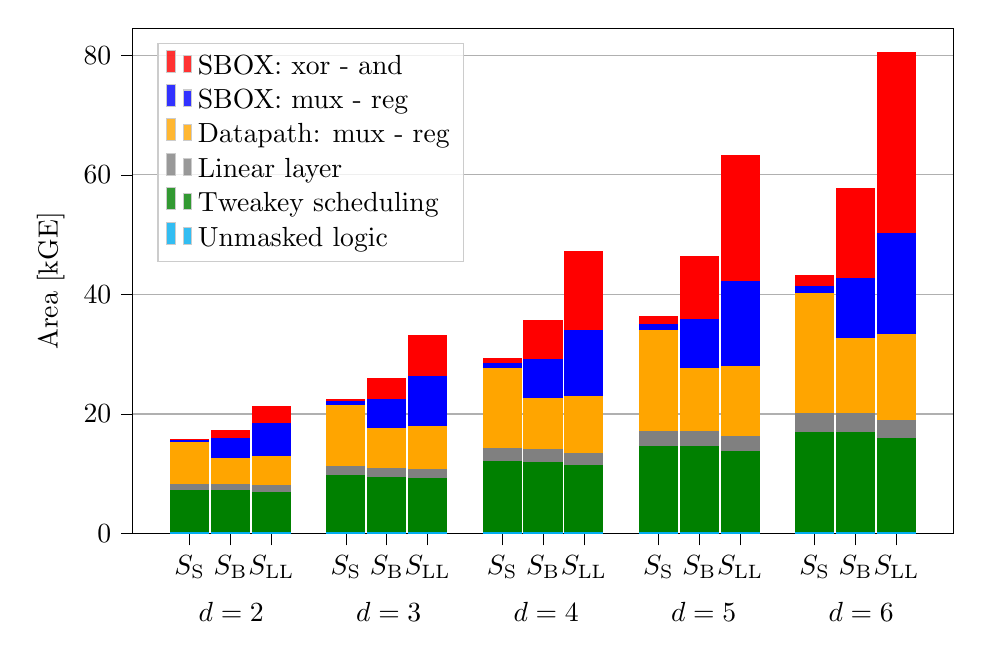
\begin{tikzpicture}
\definecolor{color0}{rgb}{1,0.647058823529412,0}

\node [] (d2) at (1.25, -1) { $d = 2$};
\node [] (d3) at (3.25, -1) { $d = 3$};
\node [] (d4) at (5.25, -1) { $d = 4$};
\node [] (d5) at (7.25, -1) { $d = 5$};
\node [] (d6) at (9.25, -1) { $d = 6$};

\begin{axis}[
height=8cm,
legend cell align={left},
legend style={
  fill opacity=0.8,
  draw opacity=1,
  text opacity=1,
  at={(0.03,0.97)},
  anchor=north west,
  draw=white!80!black
},
tick align=outside,
tick pos=left,
width=12cm,
x grid style={white!69.0196078431373!black},
xmin=1.375125, xmax=6.624875,
xtick style={color=black},
xtick={1.73875,2,2.26125,2.73875,3,3.26125,3.73875,4,4.26125,4.73875,5,5.26125,5.73875,6,6.26125},
xticklabel style={rotate=0},
xticklabels={
  \skinnys,
  \skinnyb,
  \skinnyll,
  \skinnys,
  \skinnyb,
  \skinnyll,
  \skinnys,
  \skinnyb,
  \skinnyll,
  \skinnys,
  \skinnyb,
  \skinnyll,
  \skinnys,
  \skinnyb,
  \skinnyll,
},
y grid style={white!69.0196078431373!black},
ylabel={Area [kGE]},
ymajorgrids,
ymin=0, ymax=84.5137515,
ytick style={color=black}
]
\draw[draw=none,fill=cyan] (axis cs:1.61375,0) rectangle (axis cs:1.86375,0.2166);

\addlegendimage{ybar,ybar legend,draw=none,fill=red}
\addlegendentry{SBOX: xor - and}

\addlegendimage{ybar,ybar legend,draw=none,fill=blue}
\addlegendentry{SBOX: mux - reg}

\addlegendimage{ybar,ybar legend,draw=none,fill=color0}
\addlegendentry{Datapath: mux - reg}

\addlegendimage{ybar,ybar legend,draw=none,fill=white!50.1960784313725!black}
\addlegendentry{Linear layer}

\addlegendimage{ybar,ybar legend,draw=none,fill=green!50.1960784313725!black}
\addlegendentry{Tweakey scheduling}

\addlegendimage{ybar,ybar legend,draw=none,fill=cyan}
\addlegendentry{Unmasked logic}

\draw[draw=none,fill=cyan] (axis cs:1.875,0) rectangle (axis cs:2.125,0.2166);
\draw[draw=none,fill=cyan] (axis cs:2.13625,0) rectangle (axis cs:2.38625,0.2166);
\draw[draw=none,fill=cyan] (axis cs:2.61375,0) rectangle (axis cs:2.86375,0.2166);
\draw[draw=none,fill=cyan] (axis cs:2.875,0) rectangle (axis cs:3.125,0.2166);
\draw[draw=none,fill=cyan] (axis cs:3.13625,0) rectangle (axis cs:3.38625,0.2166);
\draw[draw=none,fill=cyan] (axis cs:3.61375,0) rectangle (axis cs:3.86375,0.2166);
\draw[draw=none,fill=cyan] (axis cs:3.875,0) rectangle (axis cs:4.125,0.2166);
\draw[draw=none,fill=cyan] (axis cs:4.13625,0) rectangle (axis cs:4.38625,0.2166);
\draw[draw=none,fill=cyan] (axis cs:4.61375,0) rectangle (axis cs:4.86375,0.2166);
\draw[draw=none,fill=cyan] (axis cs:4.875,0) rectangle (axis cs:5.125,0.2166);
\draw[draw=none,fill=cyan] (axis cs:5.13625,0) rectangle (axis cs:5.38625,0.2166);
\draw[draw=none,fill=cyan] (axis cs:5.61375,0) rectangle (axis cs:5.86375,0.2166);
\draw[draw=none,fill=cyan] (axis cs:5.875,0) rectangle (axis cs:6.125,0.2166);
\draw[draw=none,fill=cyan] (axis cs:6.13625,0) rectangle (axis cs:6.38625,0.2166);
\draw[draw=none,fill=green!50.1960784313725!black] (axis cs:1.61375,0.2166) rectangle (axis cs:1.86375,7.27386928571429);

\draw[draw=none,fill=green!50.1960784313725!black] (axis cs:1.875,0.2166) rectangle (axis cs:2.125,7.26846714285714);
\draw[draw=none,fill=green!50.1960784313725!black] (axis cs:2.13625,0.2166) rectangle (axis cs:2.38625,6.99350714285714);
\draw[draw=none,fill=green!50.1960784313725!black] (axis cs:2.61375,0.2166) rectangle (axis cs:2.86375,9.76796928571429);
\draw[draw=none,fill=green!50.1960784313725!black] (axis cs:2.875,0.2166) rectangle (axis cs:3.125,9.41060357142857);
\draw[draw=none,fill=green!50.1960784313725!black] (axis cs:3.13625,0.2166) rectangle (axis cs:3.38625,9.26035142857143);
\draw[draw=none,fill=green!50.1960784313725!black] (axis cs:3.61375,0.2166) rectangle (axis cs:3.86375,12.1753628571429);
\draw[draw=none,fill=green!50.1960784313725!black] (axis cs:3.875,0.2166) rectangle (axis cs:4.125,12.0006871428571);
\draw[draw=none,fill=green!50.1960784313725!black] (axis cs:4.13625,0.2166) rectangle (axis cs:4.38625,11.4622757142857);
\draw[draw=none,fill=green!50.1960784313725!black] (axis cs:4.61375,0.2166) rectangle (axis cs:4.86375,14.5965478571429);
\draw[draw=none,fill=green!50.1960784313725!black] (axis cs:4.875,0.2166) rectangle (axis cs:5.125,14.5965478571429);
\draw[draw=none,fill=green!50.1960784313725!black] (axis cs:5.13625,0.2166) rectangle (axis cs:5.38625,13.81624);
\draw[draw=none,fill=green!50.1960784313725!black] (axis cs:5.61375,0.2166) rectangle (axis cs:5.86375,17.0075435714286);
\draw[draw=none,fill=green!50.1960784313725!black] (axis cs:5.875,0.2166) rectangle (axis cs:6.125,17.0075435714286);
\draw[draw=none,fill=green!50.1960784313725!black] (axis cs:6.13625,0.2166) rectangle (axis cs:6.38625,15.9515421428571);
\draw[draw=none,fill=white!50.1960784313725!black] (axis cs:1.61375,7.27386928571429) rectangle (axis cs:1.86375,8.33765214285714);

\draw[draw=none,fill=white!50.1960784313725!black] (axis cs:1.875,7.26846714285714) rectangle (axis cs:2.125,8.33225);
\draw[draw=none,fill=white!50.1960784313725!black] (axis cs:2.13625,6.99350714285714) rectangle (axis cs:2.38625,8.05729);
\draw[draw=none,fill=white!50.1960784313725!black] (axis cs:2.61375,9.76796928571429) rectangle (axis cs:2.86375,11.3384907142857);
\draw[draw=none,fill=white!50.1960784313725!black] (axis cs:2.875,9.41060357142857) rectangle (axis cs:3.125,10.981125);
\draw[draw=none,fill=white!50.1960784313725!black] (axis cs:3.13625,9.26035142857143) rectangle (axis cs:3.38625,10.8308728571429);
\draw[draw=none,fill=white!50.1960784313725!black] (axis cs:3.61375,12.1753628571429) rectangle (axis cs:3.86375,14.2526228571429);
\draw[draw=none,fill=white!50.1960784313725!black] (axis cs:3.875,12.0006871428571) rectangle (axis cs:4.125,14.0779471428571);
\draw[draw=none,fill=white!50.1960784313725!black] (axis cs:4.13625,11.4622757142857) rectangle (axis cs:4.38625,13.5395357142857);
\draw[draw=none,fill=white!50.1960784313725!black] (axis cs:4.61375,14.5965478571429) rectangle (axis cs:4.86375,17.1805457142857);
\draw[draw=none,fill=white!50.1960784313725!black] (axis cs:4.875,14.5965478571429) rectangle (axis cs:5.125,17.1805457142857);
\draw[draw=none,fill=white!50.1960784313725!black] (axis cs:5.13625,13.81624) rectangle (axis cs:5.38625,16.4002378571429);
\draw[draw=none,fill=white!50.1960784313725!black] (axis cs:5.61375,17.0075435714286) rectangle (axis cs:5.86375,20.09828);
\draw[draw=none,fill=white!50.1960784313725!black] (axis cs:5.875,17.0075435714286) rectangle (axis cs:6.125,20.09828);
\draw[draw=none,fill=white!50.1960784313725!black] (axis cs:6.13625,15.9515421428571) rectangle (axis cs:6.38625,19.0422785714286);
\draw[draw=none,fill=color0] (axis cs:1.61375,8.33765214285714) rectangle (axis cs:1.86375,15.2929971428571);

\draw[draw=none,fill=color0] (axis cs:1.875,8.33225) rectangle (axis cs:2.125,12.6442278571429);
\draw[draw=none,fill=color0] (axis cs:2.13625,8.05729) rectangle (axis cs:2.38625,13.0211614285714);
\draw[draw=none,fill=color0] (axis cs:2.61375,11.3384907142857) rectangle (axis cs:2.86375,21.5081285714286);
\draw[draw=none,fill=color0] (axis cs:2.875,10.981125) rectangle (axis cs:3.125,17.6026285714286);
\draw[draw=none,fill=color0] (axis cs:3.13625,10.8308728571429) rectangle (axis cs:3.38625,17.987565);
\draw[draw=none,fill=color0] (axis cs:3.61375,14.2526228571429) rectangle (axis cs:3.86375,27.731505);
\draw[draw=none,fill=color0] (axis cs:3.875,14.0779471428571) rectangle (axis cs:4.125,22.616465);
\draw[draw=none,fill=color0] (axis cs:4.13625,13.5395357142857) rectangle (axis cs:4.38625,23.0396728571429);
\draw[draw=none,fill=color0] (axis cs:4.61375,17.1805457142857) rectangle (axis cs:4.86375,33.968275);
\draw[draw=none,fill=color0] (axis cs:4.875,17.1805457142857) rectangle (axis cs:5.125,27.6558871428571);
\draw[draw=none,fill=color0] (axis cs:5.13625,16.4002378571429) rectangle (axis cs:5.38625,28.0685471428571);
\draw[draw=none,fill=color0] (axis cs:5.61375,20.09828) rectangle (axis cs:5.86375,40.190405);
\draw[draw=none,fill=color0] (axis cs:5.875,20.09828) rectangle (axis cs:6.125,32.7631778571428);
\draw[draw=none,fill=color0] (axis cs:6.13625,19.0422785714286) rectangle (axis cs:6.38625,33.3141728571429);
\draw[draw=none,fill=blue] (axis cs:1.61375,15.2929971428571) rectangle (axis cs:1.86375,15.7044257142857);

\draw[draw=none,fill=blue] (axis cs:1.875,12.6442278571429) rectangle (axis cs:2.125,15.9518564285714);
\draw[draw=none,fill=blue] (axis cs:2.13625,13.0211614285714) rectangle (axis cs:2.38625,18.5518757142857);
\draw[draw=none,fill=blue] (axis cs:2.61375,21.5081285714286) rectangle (axis cs:2.86375,22.1263);
\draw[draw=none,fill=blue] (axis cs:2.875,17.6026285714286) rectangle (axis cs:3.125,22.5665142857143);
\draw[draw=none,fill=blue] (axis cs:3.13625,17.987565) rectangle (axis cs:3.38625,26.2839364285714);
\draw[draw=none,fill=blue] (axis cs:3.61375,27.731505) rectangle (axis cs:3.86375,28.555905);
\draw[draw=none,fill=blue] (axis cs:3.875,22.616465) rectangle (axis cs:4.125,29.2363507142857);
\draw[draw=none,fill=blue] (axis cs:4.13625,23.0396728571429) rectangle (axis cs:4.38625,34.10153);
\draw[draw=none,fill=blue] (axis cs:4.61375,33.968275) rectangle (axis cs:4.86375,34.9989035714286);
\draw[draw=none,fill=blue] (axis cs:4.875,27.6558871428571) rectangle (axis cs:5.125,35.9315157142857);
\draw[draw=none,fill=blue] (axis cs:5.13625,28.0685471428571) rectangle (axis cs:5.38625,42.2296742857143);
\draw[draw=none,fill=blue] (axis cs:5.61375,40.190405) rectangle (axis cs:5.86375,41.4272621428571);
\draw[draw=none,fill=blue] (axis cs:5.875,32.7631778571428) rectangle (axis cs:6.125,42.6948064285714);
\draw[draw=none,fill=blue] (axis cs:6.13625,33.3141728571429) rectangle (axis cs:6.38625,50.31331);
\draw[draw=none,fill=red] (axis cs:1.61375,15.7044257142857) rectangle (axis cs:1.86375,15.87812);

\draw[draw=none,fill=red] (axis cs:1.875,15.9518564285714) rectangle (axis cs:2.125,17.3414107142857);
\draw[draw=none,fill=red] (axis cs:2.13625,18.5518757142857) rectangle (axis cs:2.38625,21.3309842857143);
\draw[draw=none,fill=red] (axis cs:2.61375,22.1263) rectangle (axis cs:2.86375,22.5608628571429);
\draw[draw=none,fill=red] (axis cs:2.875,22.5665142857143) rectangle (axis cs:3.125,26.0430171428571);
\draw[draw=none,fill=red] (axis cs:3.13625,26.2839364285714) rectangle (axis cs:3.38625,33.2369421428571);
\draw[draw=none,fill=red] (axis cs:3.61375,28.555905) rectangle (axis cs:3.86375,29.3749507142857);
\draw[draw=none,fill=red] (axis cs:3.875,29.2363507142857) rectangle (axis cs:4.125,35.7887164285714);
\draw[draw=none,fill=red] (axis cs:4.13625,34.10153) rectangle (axis cs:4.38625,47.2062614285714);
\draw[draw=none,fill=red] (axis cs:4.61375,34.9989035714286) rectangle (axis cs:4.86375,36.3127478571429);
\draw[draw=none,fill=red] (axis cs:4.875,35.9315157142857) rectangle (axis cs:5.125,46.44227);
\draw[draw=none,fill=red] (axis cs:5.13625,42.2296742857143) rectangle (axis cs:5.38625,63.2511828571429);
\draw[draw=none,fill=red] (axis cs:5.61375,41.4272621428571) rectangle (axis cs:5.86375,43.322925);
\draw[draw=none,fill=red] (axis cs:5.875,42.6948064285714) rectangle (axis cs:6.125,57.7911378571429);
\draw[draw=none,fill=red] (axis cs:6.13625,50.31331) rectangle (axis cs:6.38625,80.4892871428571);
\end{axis}

\end{tikzpicture}

    \caption{%
        Area requirements of leakage-resistant hardware AEAD cores in
        \SI{65}{nm} ASIC technology.
        For leveled implementations, the area is split in three part:
        DPA-protected (i.e., masked) primitives, SPA-protected primitives (implemented in parallel), and mode (i.e., logic not in a primitive).
				RN/RT respectively stand for Romulus-N/Romulus-T and A stands for Ascon.
    }
    \label{fig:modearea}
\end{figure}


Let us now discuss the area usage with \autoref{fig:modearea}.
As a general trend, for implementations with a masked primitive, the area for
that primitive dominates the overall area, with the exception of Romulus-T with
$d=2$ shares (where the area of the four non-masked Skinny instances dominates).
These results therefore confirms the interest of leveled implementations.
Next, the areas for all these modes is fairly similar, with a slight advantage
to Ascon and Romulus-N at $d=2,3$ shares thanks to their lower unmasked area, while
Romulus-T and Romulus-N are a bit better than Ascon for larger numbers of
shares, thanks to using less masked AND gadgets.
Lastly, the area for ISAP is similar to the area of the leveled implementations
with $d=2$ shares.

\section{Conclusion}

Even though the previous quantitative results should be interpreted with care, since
they explore only a few points in the design space (e.g., we considered only
round-based architectures for non-masked primitives and did not optimize the
masking randomness usage), their comparison highlights a few general trends.

\smallskip

First, for long messages, leveled implementations bring large latency
improvements while their area overheads remain small over non-leveled
implementations. This is because unmasked primitives are small compared to the masked
ones, especially when the number of shares is large.
This smaller unmasked area as well as lower latency naturally translate
into large energy savings.
The candidates that can be implemented in such a way for both
encryption and decryption (grade-2 and grade-3, see
\autoref{tab:modes_grades}) will benefit most from these savings.
However, having such mode-level characteristics usually implies more complex
modes of operations, which leads to worse performance for small messages, as
shown by the comparison between Romulus-N and the grade-2/grade-3 candidates.

\begin{table}
    \centering
    \setlength\tabcolsep{0.0em}
    \begin{tabular}{c@{\hspace{1.0em}}c@{\hspace{1.0em}}c}
        \toprule
        Grade & Security & Candidates \\
        \midrule
        0 & CCA+CI & Elephant, GIFT-COFB, Romulus-M/N, TinyJambu \\
        1 & CCAL1+CIL1 & PHOTON-Beetle, Sparkle, Xoodyak \\
        2 & CCAmL1+CIML2 & Ascon \\
        3 & CCAmL2+CIML2 & ISAP, Romulus-T \\
        \bottomrule
    \end{tabular}
    \vspace*{3ex}
    \caption{
        NIST LWC finalists grouped by mode-level leakage resistance.
    }
    \label{tab:modes_grades}\vspace*{-0.5cm}
\end{table}

Second, the leakage-resilient PRF technique used by ISAP leads to low area
implementation (similar to a leveled implementations with two shares), and
its latency is comparable to leveled implementations.
Such techniques therefore appear quite promising in hardware implementation
setting. Yet, we note that on the side-channel security side, the formal security 
guarantees of such implementations have been much less analyzed than masking
and their practical security evaluation can be more challenging as well (see, e.g.,~\cite{DBLP:conf/cosade/UdvarhelyiBS21}).


Finally, we observe that the different security margins of the algorithms we implemented
can explain some of the observed performance differences.
For example, the differences in latency between the leveled implementations of
Ascon and ISAP are explained by their number of rounds: the hashing part of ISAP
uses $\asconp^{12}$ while the Ascon inner sponge part uses only $\asconp^{6}$.
When considering CIML2, both should however withstand the same attacks.

Overall, these results backup our suggestion that
from a side-channel security viewpoint, 
the finalists of the NIST's Lightweight Crypto competition differ more 
by their qualitative features than by their quantitative performances.

%Finally qualitative properties are not free (CCAmL2, permutation vs TBC,
%flexibility w.r.t. SCA protection), so that's more the question than pure best
%performance.
%
%
%future work SW

\medskip

\noindent\textbf{Acknowledgments.} Ga\"{e}tan Cassiers and Fran\c{c}ois-Xavier Standaert are respectively
Research Fellow and Senior Associate Researcher of the Belgian Fund for Scientific
Research (FNRS-F.R.S.). This work has been funded in part by the ERC consolidator grant 
number 724725 (acronym SWORD), by the Walloon region CyberExcellence project number 2110186 (acronym Cyberwal) and by the Horizon Europe project 1010706275 (acronym REWIRE).


\bibliographystyle{alpha}
\bibliography{refs}

\end{document}
